% Final submission candidate.
\documentclass[fleqn,usenatbib]{mnras}

\usepackage{newtxtext,newtxmath}
\usepackage[T1]{fontenc}
\usepackage{ae,aecompl}

\usepackage{graphicx}
\usepackage{amsmath}
\usepackage{lastpage}
\hypersetup{hypertexnames=false}

\title[Stress-testing SURD in NGC 5548]{Stress-testing SURD for AGN Reverberation Mapping: NGC 5548}

\author[A. Mitra \& V. Zarikas]{
Ayan Mitra,$^{1}$\thanks{E-mail: ayan@illinois.edu}
Vasilios Zarikas$^{2}$
\\
$^{1}$Department of Astronomy, University of Illinois Urbana-Champaign, Urbana, IL 61801, USA\\
$^{2}$Department of Physics, University of Thessaly, Lamia 35100, Greece
}

\date{Accepted XXX. Received YYY; in original form ZZZ}
\pubyear{2026}

\begin{document}
\label{firstpage}
\pagerange{\pageref{firstpage}--\pageref{LastPage}}
\maketitle

\begin{abstract}
We stress-test multivariate information decomposition for reverberation mapping using the 5100-\AA\ continuum and velocity-resolved H$\beta$ light curves of NGC~5548. On a strict-overlap window (JD less 2400000: 47512--49255), a bidirectional interpolated cross-correlation analysis with flux-randomization/random-subset-sampling uncertainties gives centroid delays of $19.44^{+1.52}_{-1.49}$~d (blue wing), $22.79^{+1.85}_{-1.80}$~d (core), and $30.30^{+4.52}_{-3.62}$~d (red wing). By contrast, three-predictor Synergistic--Unique--Redundant Decomposition (SURD) scans have range-dependent maxima at 93--198~d. A matched 999-realization circular-shift test finds none significant ($p_{\rm global}=0.873$--1.000), and empirical lagwise p-values yield no Benjamini--Hochberg discoveries. Matched synthetic ablations show that histogram dimensionality, red-noise structure, the observing window, interpolation, and normalization are jointly sufficient to produce false long-lag maxima. A target-history-conditioned maximum at 73~d is also insignificant ($p_{\rm global}=0.9802$); changing between 3--8 equal-width or quantile bins moves it to 37--102~d while leaving every global test non-significant. Continuous nearest-neighbour estimates recover significant prompt multivariate dependence for all three line targets, but no significant 61--200~d or history-conditioned maximum. As an external check, native-cadence HST/COS light curves of Mrk~817 show elevated information near published ultraviolet-line delays, but unrestricted maxima are generally unstable across estimator scale and time-pairing tolerance. We conclude that the long-lag SURD features are not astrophysically established. Information-decomposition scans of irregular AGN data require matched controls, estimator cross-checks, and scan-wide significance tests before individual atoms or lags receive physical interpretation.
\end{abstract}
\begin{keywords}
galaxies: active -- galaxies: nuclei -- galaxies: individual: NGC 5548 -- galaxies: individual: Mrk 817 -- methods: statistical
\end{keywords}









\section{Introduction}

Active galactic nuclei (AGN) are powered by accretion onto supermassive black holes and radiate over a broad range of wavelengths through a compact but highly structured central engine. The standard observational picture includes an accretion disk that produces much of the optical and ultraviolet continuum, a hot corona responsible for the X-ray emission, a broad-line region (BLR) composed of dense photoionized gas moving at velocities of order \(10^3\) to \(10^4\) km s\(^{-1}\), and more distant dusty material that reprocesses the radiation field at infrared wavelengths \cite{Peterson2004,Netzer2013,Cackett2021}. Because these regions are too compact to resolve directly in most AGN, temporal variability provides one of the few effective ways to infer their sizes, structure, and coupling.

Reverberation mapping exploits the fact that fluctuations in the central ionizing source are echoed by delayed responses in remote reprocessing or emission-line regions. In its simplest linearized form, the response of an emission line \(L(t)\) to a driving continuum \(C(t)\) may be written as
\begin{equation}
L(t) = \int \Psi(\tau)\,C(t-\tau)\,d\tau,
\end{equation}
where \(\Psi(\tau)\) is the transfer function or delay distribution. The classical use of this formalism has been to derive a characteristic lag \(\tau\), associate it with a BLR radius \(R \sim c\tau\), and combine that scale with the line width to estimate the black-hole mass under a virial assumption \cite{Peterson2004,BentzKatz2015}. This framework has been extremely successful and remains foundational to AGN black-hole mass scaling relations.

Nevertheless, the astrophysical interpretation of reverberation data has become progressively more subtle. The quantity that drives the broad emission lines is the ionizing continuum, particularly in the extreme ultraviolet and soft X-ray bands, whereas the continuum actually monitored in many optical reverberation campaigns is a more accessible proxy, often the flux near \(5100\) \AA. As a result, the measured lag between an observed continuum band and an emission line need not correspond to a direct causal connection between those two observables alone. Instead, both may be responding, with different delays and different filtering, to a latent radiation field that is only imperfectly traced by the observed bands \cite{Cackett2021}. The question is therefore not merely what the lag is, but whether the monitored continuum contains the relevant information needed to explain the line response.

This issue is underscored by continuum reverberation mapping. A series of high-cadence monitoring programs has revealed that ultraviolet and optical continuum bands in AGN are delayed with respect to one another, with delays that often grow systematically with wavelength as expected for a thermally stratified accretion disk. However, the measured lags are frequently larger than predicted by the simplest geometrically thin, optically thick accretion-disk models \cite{Fausnaugh2016,Fausnaugh2017,Edelson2019,Cackett2021}. These results suggest that the observed continuum variability is not fully described by a minimal reprocessing picture and may involve additional processes such as intrinsic accretion-rate fluctuations, diffuse continuum emission, complex irradiation geometry, or nontrivial radiative transfer. From the standpoint of BLR reverberation, this implies that optical continuum light curves may not be interpreted as pristine drivers without further caution.

NGC~5548 is the canonical source in which these concerns become impossible to ignore. It is one of the most intensively monitored Seyfert galaxies and has served as a cornerstone of reverberation mapping for decades. It has played a major role in calibrating broad-line lags, virial mass estimates, and radius--luminosity relations, while more recent campaigns have transformed it into a benchmark for multiwavelength and velocity-resolved reverberation analysis \cite{Peterson2002,BentzKatz2015,Cackett2021}. In particular, the AGN STORM campaign delivered one of the richest reverberation datasets ever obtained, including optical and ultraviolet continuum monitoring, extensive spectroscopy, and detailed velocity-delay information for several broad lines \cite{DeRosa2015,Pei2017,Horne2021}.

These observations revealed that NGC~5548 is not well described by a stationary one-zone BLR driven by a single observed continuum proxy. Velocity-resolved reverberation results showed clear structure across the H$\beta$ profile, with the line wings and core participating differently in the reverberation pattern \cite{Pei2017,Horne2021}. The interpretation of these data points toward a BLR that is radially stratified and kinematically complex, possibly including multiple components or zones rather than a single homogeneous distribution of clouds \cite{Horne2021,LongDexter2025}. This immediately motivates a shift away from purely integrated-line analyses. If the blue wing, line core, and red wing carry different dynamical information, then treating H$\beta$ as a single scalar time series necessarily compresses part of the astrophysical content of the data.

An even more striking complication emerged during the same source's monitoring history: the so-called ``holiday'' in NGC~5548. During part of the AGN STORM campaign, the broad emission lines became partially decorrelated from the observed UV continuum, even though they had previously tracked it closely. The leading interpretation is that an obscuring wind or shielding structure modified the ionizing spectral energy distribution reaching the BLR while leaving the observed UV continuum comparatively unaffected \cite{Dehghanian2019}. The importance of this result cannot be overstated. It demonstrates directly that an observed continuum channel may cease to be a faithful tracer of the radiation field relevant for BLR photoionization. Consequently, a line--continuum lag analysis may look physically incomplete not because the line has stopped reverberating, but because the monitored continuum is no longer the appropriate driver proxy.

This broader lesson is now reinforced by work across the reverberation-mapping literature. Velocity-resolved H$\beta$ studies increasingly show that BLR kinematics are diverse across AGN and may evolve over time, with some sources displaying signatures consistent with inflow, others with outflow, and others with virialized or mixed dynamics \cite{Du2018,Wang2025,Feng2024}. In parallel, changing-look AGN have demonstrated that the relation between continuum state and broad-line emission can undergo dramatic reorganization on humanly accessible timescales \cite{RicciTrakhtenbrot2023}. Although changing-look phenomena are not the focus of the present study, they help establish a wider astrophysical principle: the mapping between observed continuum, ionizing continuum, and line-emitting gas is not guaranteed to be stationary.

Within this context, NGC~5548 is particularly well suited for a conservative test of multivariate reverberation analysis. The source offers high-quality continuum monitoring, extensive H$\beta$ spectroscopy, and a rich legacy of prior lag measurements against which information-based diagnostics can be checked. Treating the blue wing, core, and red wing as distinct observables permits questions about joint predictability that an integrated line curve cannot address. It also creates substantial statistical risk: autocorrelation, seasonal gaps, interpolation, multiple lag searches, and high-dimensional density estimation can all generate apparent structure. NGC~5548 therefore provides both an astrophysical application and a demanding stress test of the method.

These questions are not purely methodological. They arise naturally from long-standing astrophysical uncertainties about the BLR and the continuum source. The BLR is expected to be sensitive to the ionizing continuum, but in practice the ionizing continuum is usually unobserved. The optical continuum is measurable but is itself part of a reverberating accretion-flow system and may therefore contain both intrinsic and reprocessed variability components \cite{Fausnaugh2017,Cackett2021}. The H$\beta$ line is observable with high fidelity, but its integrated flux merges together multiple kinematic regions whose relative responses may differ. Once velocity-resolved spectroscopy is available, the astrophysical challenge becomes one of causal disentanglement among observables that are neither independent nor trivially ordered in a simple driver--response chain.

A number of established approaches address parts of this challenge. Interpolated cross-correlation methods and related lag estimators remain the standard tools for continuum--line reverberation analysis and continue to provide essential baseline measurements \cite{Peterson2004,WhitePeterson1994}. JAVELIN and related stochastic-process approaches model reverberation as a damped random walk continuum filtered by a transfer function, thereby improving lag estimation and uncertainty quantification in many cases \cite{Zu2011,Zu2013}. Velocity-delay mapping and dynamical modeling aim to reconstruct the geometry and kinematics of the BLR directly from the line-profile response \cite{Pancoast2014,Horne2021}. Continuum reverberation studies focus on interband disk lags and the thermal structure of the accretion flow \cite{Fausnaugh2016,Fausnaugh2017,Edelson2019}. Each of these approaches has been productive, but they are typically tailored to a specific projection of the problem: pairwise lags, transfer-function fitting, dynamical inversion, or continuum size scaling.

What remains comparatively underexplored is the specific astrophysical question of how multiple simultaneously observed channels jointly constrain the future evolution of one chosen component of the system, especially when those channels include both the continuum and velocity-resolved line segments. In other words, once the H$\beta$ profile has been decomposed into blue wing, core, and red wing light curves, and once a conservative common time interval is imposed, the natural problem is no longer simply ``what is the lag?'' It becomes: how much of the future behavior of one velocity component is already encoded in the continuum, how much is encoded in another part of the line profile, and how much lies beyond the information available in the monitored observables? That is the astrophysical problem motivating the present paper.

The emphasis on strict temporal overlap is also not incidental. Irregular cadence, seasonal gaps, and unequal overlap among observed channels are intrinsic features of AGN monitoring data. Any multivariate time-series analysis is therefore vulnerable to spurious structure introduced by aggressive interpolation, extrapolation across gaps, or implicit assumptions about the simultaneity of channels that were not truly observed together. In the context of NGC~5548, where the scientific questions depend sensitively on comparing the optical continuum to distinct H$\beta$ velocity components, it is essential to work under conservative overlap conditions. The goal is not to maximize sample size at all costs, but to preserve physical interpretability. A shorter but genuinely shared time interval is preferable to a longer one in which apparent multivariate structure may be partly synthetic.

The aim of this paper is to determine which conclusions from a multivariate SURD analysis remain defensible after conservative temporal overlap, synthetic recovery tests, red-noise-preserving global nulls, discretization sensitivity, and a continuous-estimator cross-check. We retain the blue wing, line core, and red wing as separate channels, but treat any inferred atom or lag as exploratory unless it is stable under those controls.

The methodological framework used later in the paper is based on information decomposition, but we intentionally postpone its formal description. The present Introduction has a different role: to show why such an analysis is astrophysically warranted. The literature has already established that NGC~5548 exhibits continuum interband lags, velocity-resolved H$\beta$ structure, partial line--continuum decoupling during the holiday, and evidence for a multicomponent BLR. The natural next step is not simply to add another lag estimator, but to investigate the reverberation data in a way that is explicitly multivariate, velocity-resolved, and conservative with respect to temporal overlap. That is the problem we address here.

The structure of this paper is as follows. Section~2 introduces the information framework; Section~3 describes the observations and strict-overlap processing; Section~4 presents the tests and results; Section~5 discusses their implications; and Section~6 summarizes the conclusions.


\section{Synergistic--Unique--Redundant Decomposition (SURD) for Time Series}
\label{sec:surd_method}

\subsection{Problem formulation}

Consider a collection of \(N\) observed stochastic processes,
\begin{equation}
\mathbf{Q}(t)=\bigl(Q_1(t),Q_2(t),\ldots,Q_N(t)\bigr),
\end{equation}
sampled at discrete times \(t=t_n\). For a chosen target index \(j\), the goal is to quantify how much information about the future state
\begin{equation}
Q_j^+ \equiv Q_j(t+\Delta T)
\end{equation}
is contained in the observed variables at time \(t\) and, crucially, to decompose that predictive information into \emph{redundant}, \emph{unique}, and \emph{synergistic} contributions \cite{MartinezSanchez2024SURD}.

The central motivation is that in multivariate systems, pairwise predictive measures such as Granger causality or transfer entropy can establish that a variable is informative about a target, but they do not in general distinguish whether that information is:
\begin{enumerate}
    \item unique to one predictor,
    \item duplicated across several predictors, or
    \item available only from a joint observation of several predictors.
\end{enumerate}
SURD is designed precisely to perform that decomposition in a time-series setting \cite{MartinezSanchez2024SURD,Schreiber2000,WilliamsBeer2010}.

\subsection{Information-theoretic preliminaries}

Let \(Y\equiv Q_j^+\) denote the target and let \(\mathbf{X}\) denote the vector of observed predictors. For discrete variables, the Shannon entropy is
\begin{equation}
H(Y)=-\sum_{y} p(y)\log_2 p(y),
\end{equation}
and the conditional entropy of \(Y\) given \(\mathbf{X}\) is
\begin{equation}
H(Y\mid \mathbf{X})=-\sum_{y,\mathbf{x}} p(y,\mathbf{x})\log_2 p(y\mid \mathbf{x}).
\end{equation}
The mutual information between \(Y\) and \(\mathbf{X}\) is
\begin{equation}
I(Y;\mathbf{X})=H(Y)-H(Y\mid \mathbf{X})
=\sum_{y,\mathbf{x}} p(y,\mathbf{x})
\log_2\frac{p(y,\mathbf{x})}{p(y)p(\mathbf{x})}.
\label{eq:mi_total}
\end{equation}
This quantity measures the total predictive information about the future target that is available in the observed present state \cite{Shannon1948,CoverThomas2006}.

In SURD, the unexplained part of the future is interpreted as an \emph{information leak},
\begin{equation}
\Delta I_{\mathrm{leak}\to j}=H(Y\mid \mathbf{X}),
\label{eq:leak_def}
\end{equation}
so that the forward information balance reads
\begin{equation}
H(Y)=I(Y;\mathbf{X})+\Delta I_{\mathrm{leak}\to j}.
\label{eq:forward_balance}
\end{equation}

Equation \eqref{eq:forward_balance} is one of the core ideas of SURD: the future uncertainty of the target splits into an observed part, explained by the measured variables, and an unobserved part, attributed to hidden or unmeasured influences \cite{MartinezSanchez2024SURD}.

\subsection{From total predictive information to information-decomposition components}

Let the predictor vector be
\begin{equation}
\mathbf{X} = (X_1,\ldots,X_M),
\end{equation}
where the \(X_\alpha\) may correspond either to different physical variables at the same time, or to different lagged copies of the same variables. SURD decomposes the observable predictive information \(I(Y;\mathbf{X})\) into additive components:
\begin{equation}
I(Y;\mathbf{X})
=
\sum_{\mathcal{A}\in\mathcal{C}} \Delta I_{\mathcal{A}\to j}^{R}
+
\sum_{\alpha=1}^{M} \Delta I_{\alpha\to j}^{U}
+
\sum_{\mathcal{A}\in\mathcal{C}} \Delta I_{\mathcal{A}\to j}^{S},
\label{eq:surd_master}
\end{equation}
where:
\begin{itemize}
    \item \(\Delta I_{\mathcal{A}\to j}^{R}\) is the \emph{redundant} contribution from the group of predictors indexed by \(\mathcal{A}\),
    \item \(\Delta I_{\alpha\to j}^{U}\) is the \emph{unique} contribution of predictor \(X_\alpha\),
    \item \(\Delta I_{\mathcal{A}\to j}^{S}\) is the \emph{synergistic} contribution from the group \(\mathcal{A}\),
    \item \(\mathcal{C}\) denotes all non-singleton subsets of \(\{1,\dots,M\}\).
\end{itemize}
The full future entropy therefore obeys
\begin{equation}
H(Y)=
\sum_{\mathcal{A}\in\mathcal{C}} \Delta I_{\mathcal{A}\to j}^{R}
+
\sum_{\alpha=1}^{M} \Delta I_{\alpha\to j}^{U}
+
\sum_{\mathcal{A}\in\mathcal{C}} \Delta I_{\mathcal{A}\to j}^{S}
+
\Delta I_{\mathrm{leak}\to j}.
\label{eq:full_surd_balance}
\end{equation}

The three information-decomposition types have the following interpretation \cite{MartinezSanchez2024SURD}:
\begin{itemize}
\item{Redundant:}  
the same predictive information is shared across several predictors,\\
\item{Unique:}  
a predictor contains information not available from any other predictor alone,\\
\item {Synergistic:}  
information appears only when several predictors are observed jointly.
\end{itemize}

For the three-predictor scans below, ``total synergy'' denotes
$S_{12}+S_{13}+S_{23}+S_{123}$ and ``total redundancy'' denotes
$R_{12}+R_{13}+R_{23}+R_{123}$. These sums, rather than any single atom,
are the quantities shown in the primary lag scans.

\iffalse
\subsection{Specific mutual information and statewise decomposition}

A key feature of SURD is that the source of predictability may depend on which \emph{particular future event} \(y\) occurs. To resolve this dependence, SURD works first at the level of \emph{specific mutual information} \cite{DeWeeseMeister1999,Butts2003,MartinezSanchez2024SURD}.

For a particular target state \(Y=y\), the specific mutual information between \(y\) and a predictor set \(\mathbf{X}_{\mathcal{A}}\) is
\begin{equation}
\tilde{\imath}_{\mathcal{A}}(y)
\equiv
\tilde{\imath}\bigl(y;\mathbf{X}_{\mathcal{A}}\bigr)
=
\sum_{\mathbf{x}_{\mathcal{A}}}
\frac{p(y,\mathbf{x}_{\mathcal{A}})}{p(y)}
\log_2
\frac{p(y,\mathbf{x}_{\mathcal{A}})}{p(y)\,p(\mathbf{x}_{\mathcal{A}})}.
\label{eq:specific_mi}
\end{equation}
The ordinary mutual information is recovered by averaging over target states:
\begin{equation}
I\bigl(Y;\mathbf{X}_{\mathcal{A}}\bigr)
=
\sum_{y} p(y)\,\tilde{\imath}_{\mathcal{A}}(y).
\label{eq:mi_from_specific}
\end{equation}

The conceptual reason for introducing \(\tilde{\imath}_{\mathcal{A}}(y)\) is that different predictors may be informative for different target outcomes. A predictor may, for example, strongly constrain large positive target excursions while another may mainly constrain negative or low-amplitude states. A decomposition performed only at the level of the average mutual information can obscure this state dependence. SURD therefore computes the information contributions for each \(y\), decomposes them into redundant, unique, and synergistic increments, and only afterwards averages over \(y\) \cite{MartinezSanchez2024SURD}.

\subsection{Statewise incremental construction of SURD}

Let \(\mathfrak{P}^\ast(\{1,\dots,M\})\) denote the set of all non-empty subsets of predictors. For each subset \(\mathcal{A}\in \mathfrak{P}^\ast(\{1,\dots,M\})\), one computes
\begin{equation}
\tilde{\imath}_{\mathcal{A}}(y)
=
\tilde{\imath}\bigl(y;\mathbf{X}_{\mathcal{A}}\bigr).
\end{equation}
SURD then considers the collection of all these values for a fixed target state \(y\) and identifies the \emph{increments} in predictive information that arise as one moves from smaller to larger subsets of predictors \cite{MartinezSanchez2024SURD}. Denoting these statewise increments schematically by
\begin{equation}
\Delta \tilde{\imath}_{\mathcal{A}}(y),
\end{equation}
the classification rule is:
\begin{itemize}
    \item an increment assigned to one predictor alone contributes to \(\Delta \tilde{\imath}_{\alpha}^{U}(y)\),
    \item an increment shared across several predictors contributes to \(\Delta \tilde{\imath}_{\mathcal{A}}^{R}(y)\),
    \item an increment that arises only when a collection of predictors is observed jointly contributes to \(\Delta \tilde{\imath}_{\mathcal{A}}^{S}(y)\).
\end{itemize}

The averaged decomposed components are then
\begin{align}
\Delta I_{\mathcal{A}\to j}^{R}
&=
\sum_{y} p(y)\,\Delta \tilde{\imath}_{\mathcal{A}}^{R}(y),\\
\Delta I_{\alpha\to j}^{U}
&=
\sum_{y} p(y)\,\Delta \tilde{\imath}_{\alpha}^{U}(y),\\
\Delta I_{\mathcal{A}\to j}^{S}
&=
\sum_{y} p(y)\,\Delta \tilde{\imath}_{\mathcal{A}}^{S}(y).
\end{align}
This construction ensures that the total observable predictive information is recovered exactly:
\begin{equation}
I(Y;\mathbf{X})
=
\sum_{\mathcal{A}\in\mathcal{C}} \Delta I_{\mathcal{A}\to j}^{R}
+
\sum_{\alpha=1}^{M} \Delta I_{\alpha\to j}^{U}
+
\sum_{\mathcal{A}\in\mathcal{C}} \Delta I_{\mathcal{A}\to j}^{S}.
\label{eq:observable_recovery}
\end{equation}

\subsection{Two-source case}

For two predictors \(X_1\) and \(X_2\), the decomposition reduces to
\begin{equation}
I(Y;X_1,X_2)
=
\Delta I_{12\to j}^{R}
+
\Delta I_{1\to j}^{U}
+
\Delta I_{2\to j}^{U}
+
\Delta I_{12\to j}^{S}.
\label{eq:two_source_total}
\end{equation}
Consistency with the single-predictor mutual informations requires
\begin{align}
I(Y;X_1) &= \Delta I_{12\to j}^{R} + \Delta I_{1\to j}^{U},\\
I(Y;X_2) &= \Delta I_{12\to j}^{R} + \Delta I_{2\to j}^{U}.
\end{align}
Hence the synergistic contribution may be written as the remainder
\begin{equation}
\Delta I_{12\to j}^{S}
=
I(Y;X_1,X_2)
-
\Delta I_{12\to j}^{R}
-
\Delta I_{1\to j}^{U}
-
\Delta I_{2\to j}^{U}.
\end{equation}
This form makes the interpretation transparent: the synergy is the part of the joint predictive information that cannot be accounted for by the redundant and unique terms.

\subsection{Extension to time series with multiple lags}

For time-series applications, the predictor vector is typically augmented with lagged copies of the observed variables. If one includes \(p\) past lags per variable, the predictor vector becomes
\begin{equation}
\begin{split}
\mathbf{X}(t) = \Bigl[ & Q_1(t), Q_1(t-\Delta T_1), \ldots, Q_1(t-\Delta T_p), \\
                       & Q_2(t), Q_2(t-\Delta T_1), \ldots, Q_N(t-\Delta T_p) \Bigr].
\end{split}
\label{eq:lagged_vector_general}
\end{equation}
For example, with \(N=2\) variables and one additional lag,
\begin{equation}
\mathbf{X}(t)=
\bigl[
Q_1(t),Q_1(t-\Delta T),Q_2(t),Q_2(t-\Delta T)
\bigr].
\label{eq:lagged_vector_two}
\end{equation}
SURD then treats each lagged component as one predictor channel and applies the same decomposition machinery to the enlarged predictor set \cite{MartinezSanchez2024SURD}. In this way, the method can distinguish:
\begin{itemize}
    \item self-causation from \(Q_j(t-\Delta T_k)\) to \(Q_j(t+\Delta T)\),
    \item cross-causation from \(Q_i(t-\Delta T_k)\) to \(Q_j(t+\Delta T)\),
    \item redundancy between different lags,
    \item synergy between variables and lags.
\end{itemize}

This is particularly important when several lagged channels may encode overlapping predictive content. For example, adding \(Q_j(t)\) and \(Q_j(t-\Delta T)\) can increase redundancy rather than revealing new independent predictive pathways. SURD is expressly designed to make that distinction \cite{MartinezSanchez2024SURD}.

\subsection{Contemporaneous and mixed lagged dependencies}

A further advantage of the formalism is that the predictor vector can include variables at time \(t+\Delta T\) other than the target itself, thereby allowing the analysis of contemporaneous or effectively sub-resolution interactions \cite{MartinezSanchez2024SURD}. In practice, one excludes the target variable from the contemporaneous predictor set to avoid trivial self-determination, but permits other variables measured on the same time slice. Thus, a generic predictor vector may mix present, lagged, and contemporaneous channels:
\begin{equation}
\begin{split}
\mathbf{X}(t) = \bigl[ & \text{past lags}, \text{ present variables}, \\
                       & \text{contemporaneous non-target variables} \bigr].
\end{split}
\end{equation}
The same decomposition \eqref{eq:full_surd_balance} then applies.

\fi
The statewise construction and detailed lagged formalism follow \citet{MartinezSanchez2024SURD}; we omit that derivation here and retain only the quantities required for the analysis.

\subsection{Normalization and interpretation}

Because the observable predictive information is conserved by construction, the unique, redundant, and synergistic terms are naturally normalized by the total observable mutual information:
\begin{equation}
\begin{aligned}
\widehat{\Delta I}_{\mathcal{A}\to j}^{R}
&=\frac{\Delta I_{\mathcal{A}\to j}^{R}}{I(Y;\mathbf{X})},\\
\widehat{\Delta I}_{\alpha\to j}^{U}
&=\frac{\Delta I_{\alpha\to j}^{U}}{I(Y;\mathbf{X})},\\
\widehat{\Delta I}_{\mathcal{A}\to j}^{S}
&=\frac{\Delta I_{\mathcal{A}\to j}^{S}}{I(Y;\mathbf{X})}.
\end{aligned}
\label{eq:normalized_atoms}
\end{equation}
These normalized terms sum to unity:
\begin{equation}
\sum_{\mathcal{A}\in\mathcal{C}}\widehat{\Delta I}_{\mathcal{A}\to j}^{R}
+
\sum_{\alpha=1}^{M}\widehat{\Delta I}_{\alpha\to j}^{U}
+
\sum_{\mathcal{A}\in\mathcal{C}}\widehat{\Delta I}_{\mathcal{A}\to j}^{S}
=1.
\end{equation}
The leak is normalized instead by the total entropy of the target:
\begin{equation}
\widehat{\Delta I}_{\mathrm{leak}\to j}
=
\frac{\Delta I_{\mathrm{leak}\to j}}{H(Y)}
=
\frac{H(Y\mid\mathbf{X})}{H(Y)}.
\label{eq:normalized_leak}
\end{equation}
Hence:
\begin{itemize}
    \item \(\widehat{\Delta I}_{\mathrm{leak}\to j}\approx 0\) means the observed predictors account for almost all predictive information about the target,
    \item \(\widehat{\Delta I}_{\mathrm{leak}\to j}\approx 1\) means most of the target's future uncertainty remains unexplained by the observed variables.
\end{itemize}

\subsection{Practical estimation}

In applications, the probabilities entering Eq.~\eqref{eq:mi_total} and the statewise SURD construction must be estimated from finite data. The original SURD work uses histogram-based and transport-map-based estimators depending on dimensionality and sample size \cite{MartinezSanchez2024SURD}. In a histogram implementation, one discretizes the predictor-target space into bins and estimates
\begin{equation}
p(y,\mathbf{x}) \approx \frac{n(y,\mathbf{x})}{N_{\mathrm{samples}}},
\end{equation}
where \(n(y,\mathbf{x})\) is the bin count. The resulting empirical joint distribution is then used to compute all required marginal and conditional probabilities. More sophisticated estimators, such as transport maps, are advantageous in high dimensions because the number of bins required by direct histograms grows exponentially with the number of predictors.

Algorithmically, the SURD workflow for a target \(Q_j^+\) is:
\begin{enumerate}
    \item choose the predictor vector \(\mathbf{X}\), including variables, lags, or contemporaneous channels;
    \item estimate the probability distributions \(p(y,\mathbf{x}_{\mathcal{A}})\) for all relevant predictor subsets \(\mathcal{A}\);
    \item compute the specific informations \(\tilde{\imath}_{\mathcal{A}}(y)\) for every target state \(y\);
    \item decompose the statewise increments into redundant, unique, and synergistic parts;
    \item average over \(y\) to obtain \(\Delta I^R\), \(\Delta I^U\), and \(\Delta I^S\);
    \item compute the leak from Eq.~\eqref{eq:leak_def};
    \item normalize the observable components by \(I(Y;\mathbf{X})\) and the leak by \(H(Y)\).
\end{enumerate}

\iffalse
\subsection{Properties and assumptions}

SURD has several properties that are important in time-series applications \cite{MartinezSanchez2024SURD}:
\begin{enumerate}
    \item \textbf{Non-negativity:} all redundant, unique, synergistic, and leak terms are non-negative.
    \item \textbf{Additivity:} the observable predictive information is exactly partitioned into \(R\), \(U\), and \(S\) terms.
    \item \textbf{Sensitivity to nonlinear dependence:} because the construction is based on mutual information, it is not restricted to linear couplings.
    \item \textbf{Compatibility with lagged and contemporaneous predictors:} time-lag structure enters through the predictor vector.
    \item \textbf{Hidden-variable diagnostics:} the leak quantifies the fraction of future uncertainty left unexplained by the observed variables.
\end{enumerate}

The main assumptions are those common to observational information-theoretic analysis:
\begin{itemize}
    \item the processes are sufficiently stationary over the analysis interval for probability estimation to be meaningful,
    \item the chosen time resolution is physically relevant,
    \item the sample size is adequate for the selected probability estimator,
    \item and statistical interpretation remains limited to the observed variables plus the quantified unresolved contribution represented by the leak.
\end{itemize}

\subsection{Summary}

SURD starts from the predictive information \(I(Q_j^+;\mathbf{X})\) between a future target and a multivariate predictor state. It then decomposes that predictive information into state-averaged unique, redundant, and synergistic contributions, while retaining the conditional entropy \(H(Q_j^+\mid \mathbf{X})\) as an explicit measure of hidden or unobserved influence. Its time-series extension is straightforward: past lags, present variables, and even contemporaneous non-target channels are simply incorporated into the predictor vector. For multivariate dynamical systems, this yields a decomposition that is richer than pairwise lag measures because it distinguishes direct predictive effects from duplicated information and from genuinely joint multivariate effects \cite{MartinezSanchez2024SURD,WilliamsBeer2010}.

\fi
\section{Adopted Data, Spectral Processing, and Sampling Validation}
\label{sec:data_processing}

The adopted reduction uses 242 H$\beta$ spectra on 224 distinct dates. Of the 247 archived profiles, five lack an exact date and instrument match in corrected Table 1 of \citet{WandersPeterson1996} and are excluded under a documented provenance policy. These are \texttt{n57653ab.spc}, \texttt{n57654ab.spc}, \texttt{n57657ab.spc}, \texttt{n57711ab.spc}, and \texttt{n57725ab.spc}. Their original files are preserved; the exclusion does not establish that their measurements are invalid.

We express dates as JD less 2400000, rather than MJD. The revised continuum file requires 40000 to be added to its tabulated dates, despite the archive landing page stating the other convention. All 242 selected dates and revised continuum fluxes have unique matches in the corrected table within the documented flux tolerance of 0.00051 in the revised archive units. Spectral dates have integer day precision; the precise time scale and correction to the heliocentre remain unspecified.

The adopted velocity intervals are $[-6000,-2000)$, $[-2000,2000)$ and $[2000,6000)$~$\mathrm{km\,s^{-1}}$ for the blue wing, core and red wing respectively. We use observed wavelengths with reference wavelength 4861.33~\AA\ and numerical reference redshift 0.017175. These conventions retain the existing project reduction; they are not the exact intervals or redshift used in the source paper. Each selected pixel contributes its flux density multiplied by its 2~\AA\ width. Profiles are in arbitrary flux density units, so the resulting components are in arbitrary integrated units.

Measurements sharing a date are averaged with equal weights for all components, preserving the identity between their sum and the integrated selected profile. Errors propagate in quadrature under independence assumptions. Pixel covariance and shared calibration covariance are unavailable. The selected profile sum differs from the archive total H$\beta$ light curve, whose subtraction conventions differ.

The original continuum remains primary for continuity and denser observed sampling. The revised continuum is retained as a sensitivity input. Its flux units and galaxy subtraction differ from the original continuum. Table~\ref{tab:adopted_inputs} separates measurement counts from distinct dates. Each series retains its observed endpoints; lagged pairing enforces the support of each required series.

\begin{table*}
\centering
\begin{tabular}{lrrrr}
\hline
Series & Measurements & Dates & First JD offset & Last JD offset \\
\hline
H$\beta$ components & 242 & 224 & 47512.00 & 49255.00 \\
Original continuum & 557 & 557 & 47512.00 & 49243.66 \\
Revised continuum & 242 & 224 & 47512.00 & 49255.00 \\
\hline
\end{tabular}
\caption{Adopted input counts and actual support endpoints. JD offsets are relative to 2400000. The revised continuum is a sensitivity input.}
\label{tab:adopted_inputs}
\end{table*}

We compare a daily linear interpolation grid, interpolation restricted to gaps of at most 30 days, analysis within seasons divided at gaps exceeding 60 days in either input and also restricted to 30 day interpolation gaps, and native observation pairing with a one day tolerance. Native ties select the earlier observation. No method extrapolates. A positive lag places the line target after its predictors. A native target contributes at most one tuple at each lag, although predictor observations may be reused. Counts therefore do not represent independent sample sizes (Table~\ref{tab:adopted_sampling_counts}).

\begin{table*}
\centering
\begin{tabular}{rrrrr}
\hline
Lag (days) & Daily & Limited gaps & Within seasons & Native \\
\hline
0 & 1732 & 1363 & 1363 & 223 \\
30 & 1714 & 1174 & 1174 & 74 \\
100 & 1644 & 980 & 980 & 60 \\
200 & 1544 & 840 & 778 & 51 \\
\hline
\end{tabular}
\caption{Lagged tuple counts under the adopted sampling rules. There are 224 native line dates and 557 original continuum dates.}
\label{tab:adopted_sampling_counts}
\end{table*}

The exploratory information pilot scans 201 lags from zero through 200 days for three line targets. Each target uses continuum and the other two line components at a common lag as predictors; the target component is excluded at every lag. Four marginal quantile bins are defined from native observations and held fixed across methods and lags within each dataset. The identical rule defines bins for each simulated dataset. A minimum of 32 tuples is a numerical guard, not evidence of adequate statistical support. Joint mutual information, individual SURD atoms, total synergy in bits, synergy divided by joint information, and histogram occupancy are saved separately.

Eight simulated datasets have exercised this complete execution path, using independent signals and a delayed shared continuum driver. The process parameters are stipulated and have not been fitted to the observed campaign. This is a runtime and correctness pilot, not significance calibration or a detection power measurement. The present scans do not replace the historical numerical results elsewhere in the draft. Those results must be recomputed on the adopted sample or explicitly identified as historical diagnostics before submission.

\begin{figure*}
\centering
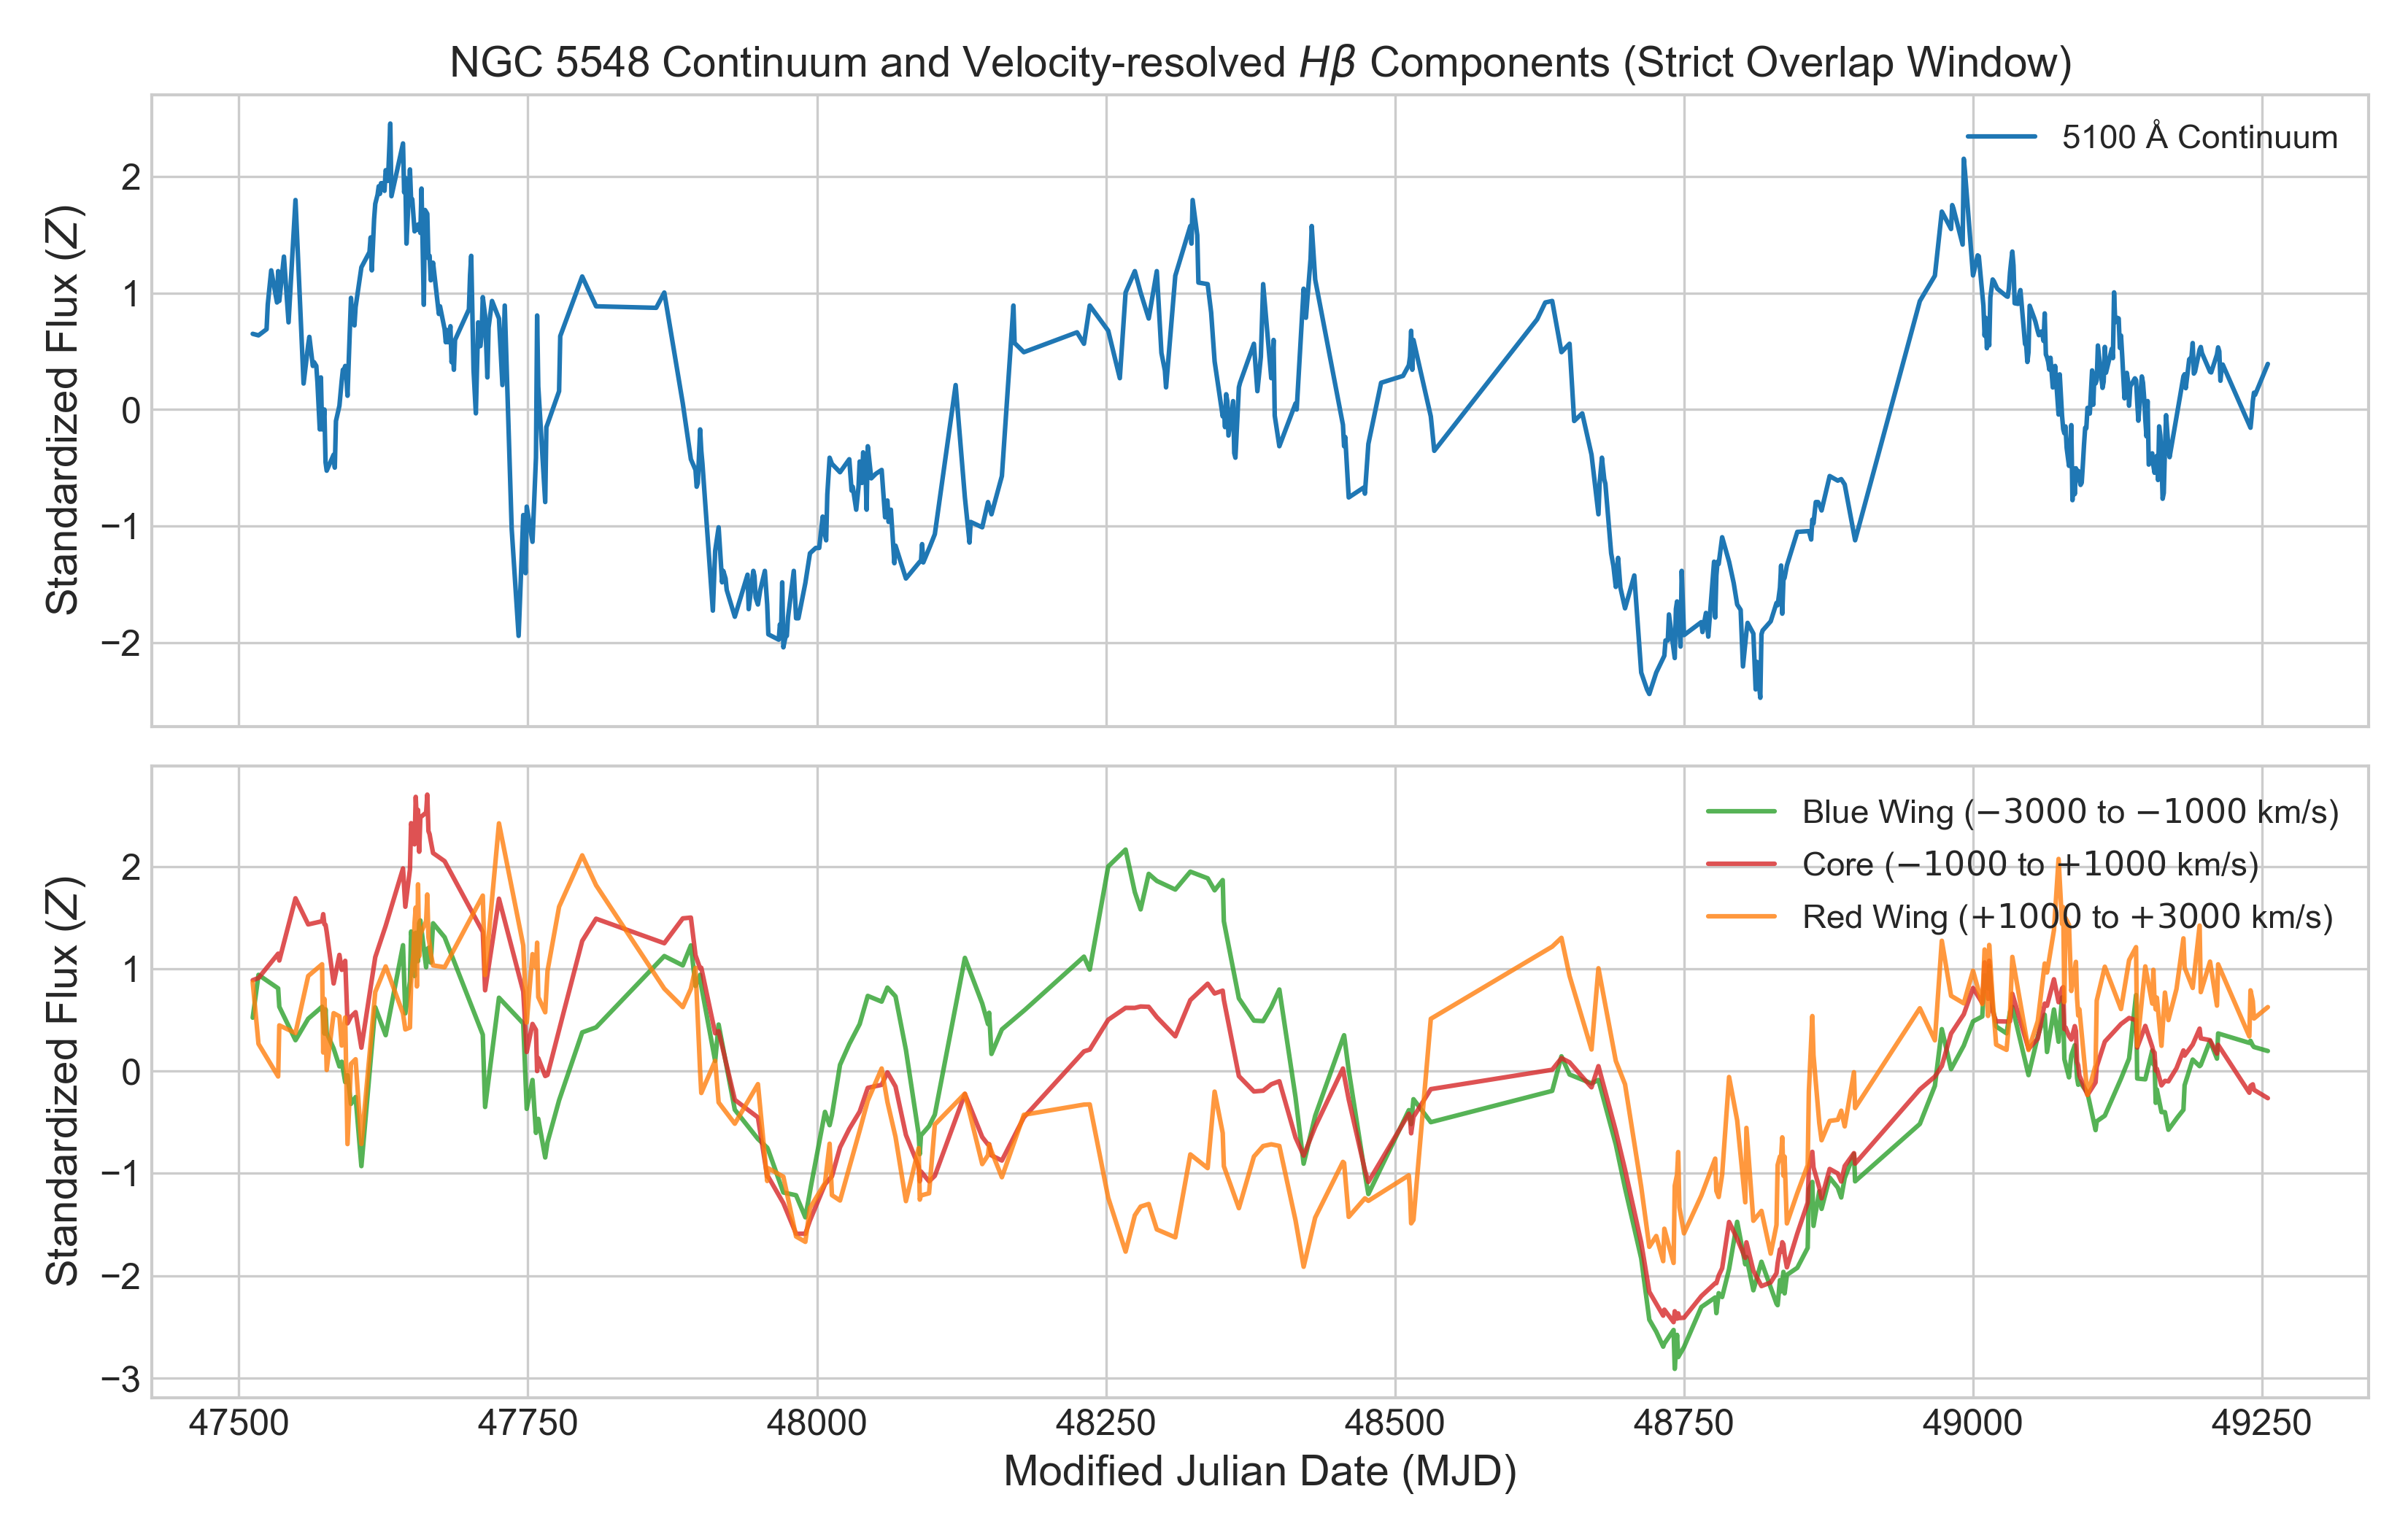
\includegraphics[width=\textwidth]{figure1_light_curves.png}
\caption{Top panel: Standardized 5100~\AA\ continuum light curve for NGC~5548 over the strictly aligned overlap window (JD less 2400000: 47512--49255). Bottom panel: Standardized velocity-resolved H\(\beta\) components (Blue Wing, Line Core, and Red Wing) resampled onto the shared 1.0-day grid.}
\label{fig:light_curves}
\end{figure*}



\section{Information Decomposition and Lag Analysis Results}
\label{sec:results}

We run the SURD algorithm in a symmetric, round-robin configuration on the prepared NGC~5548 data to study predictive dependence between the four observables: the continuum, the red and blue wings, and the core of H\(\beta\). For each run, we set one observable as the target $Y$ and use the remaining three observables as the predictor set $\mathbf{X} = \{X_1, X_2, X_3\}$. The continuum-target run is included only as a reverse-prediction diagnostic of the estimator; it is not a physical reverberation configuration in which the line drives the continuum.

\subsection{Dominant Lags and Extended Scan Range}

To test the physical stability of the synergy and leak profiles, we extended the lag search range from the initial limit of 60 days to 200 days. The comparison of peak lags and synergy values between the standard and extended scans is summarized in Table~\ref{tab:peak_synergy_comparison}, and the complete information decomposition profiles are displayed in Figure~\ref{fig:surd_lag_scans}.

\begin{table*}
\centering
\begin{tabular}{lcccc}
\hline
\textbf{Target Component} & \textbf{Old Peak Lag (d)} & \textbf{New Peak Lag (d)} & \textbf{Old Peak Synergy} & \textbf{New Peak Synergy} \\
\hline
Continuum & 34 & 115 & 0.6882 & 0.7138 \\
Red Wing H\(\beta\) & 46 & 198 & 0.7218 & 0.7358 \\
Core H\(\beta\) & 53 & 128 & 0.6330 & 0.7045 \\
Blue Wing H\(\beta\) & 56 & 93 & 0.6787 & 0.7133 \\
\hline
\end{tabular}
\caption{Comparison of peak normalized synergy lags and values between the standard (1--60 days) and extended (1--200 days) round-robin 3-predictor SURD scans. Note that the peaks shift substantially when extending the scan window, indicating that the unconditioned peak lag is scan-range-dependent and does not represent a stable physical delay.}
\label{tab:peak_synergy_comparison}
\end{table*}

For all four observables, the peak synergy lag shifts when the scan range is extended from 60 days to 200 days. Specifically, the Continuum peak shifts from 34 days to 115 days, the Red Wing peak shifts from 46 days to 198 days, the Core peak shifts from 53 days to 128 days, and the Blue Wing peak shifts from 56 days to 93 days. This variability shows that the unconditioned peaks are scan-range-dependent and do not converge on stable physical delays; boundary and windowing effects are therefore plausible alternatives to a physical interpretation.

\begin{figure*}
\centering
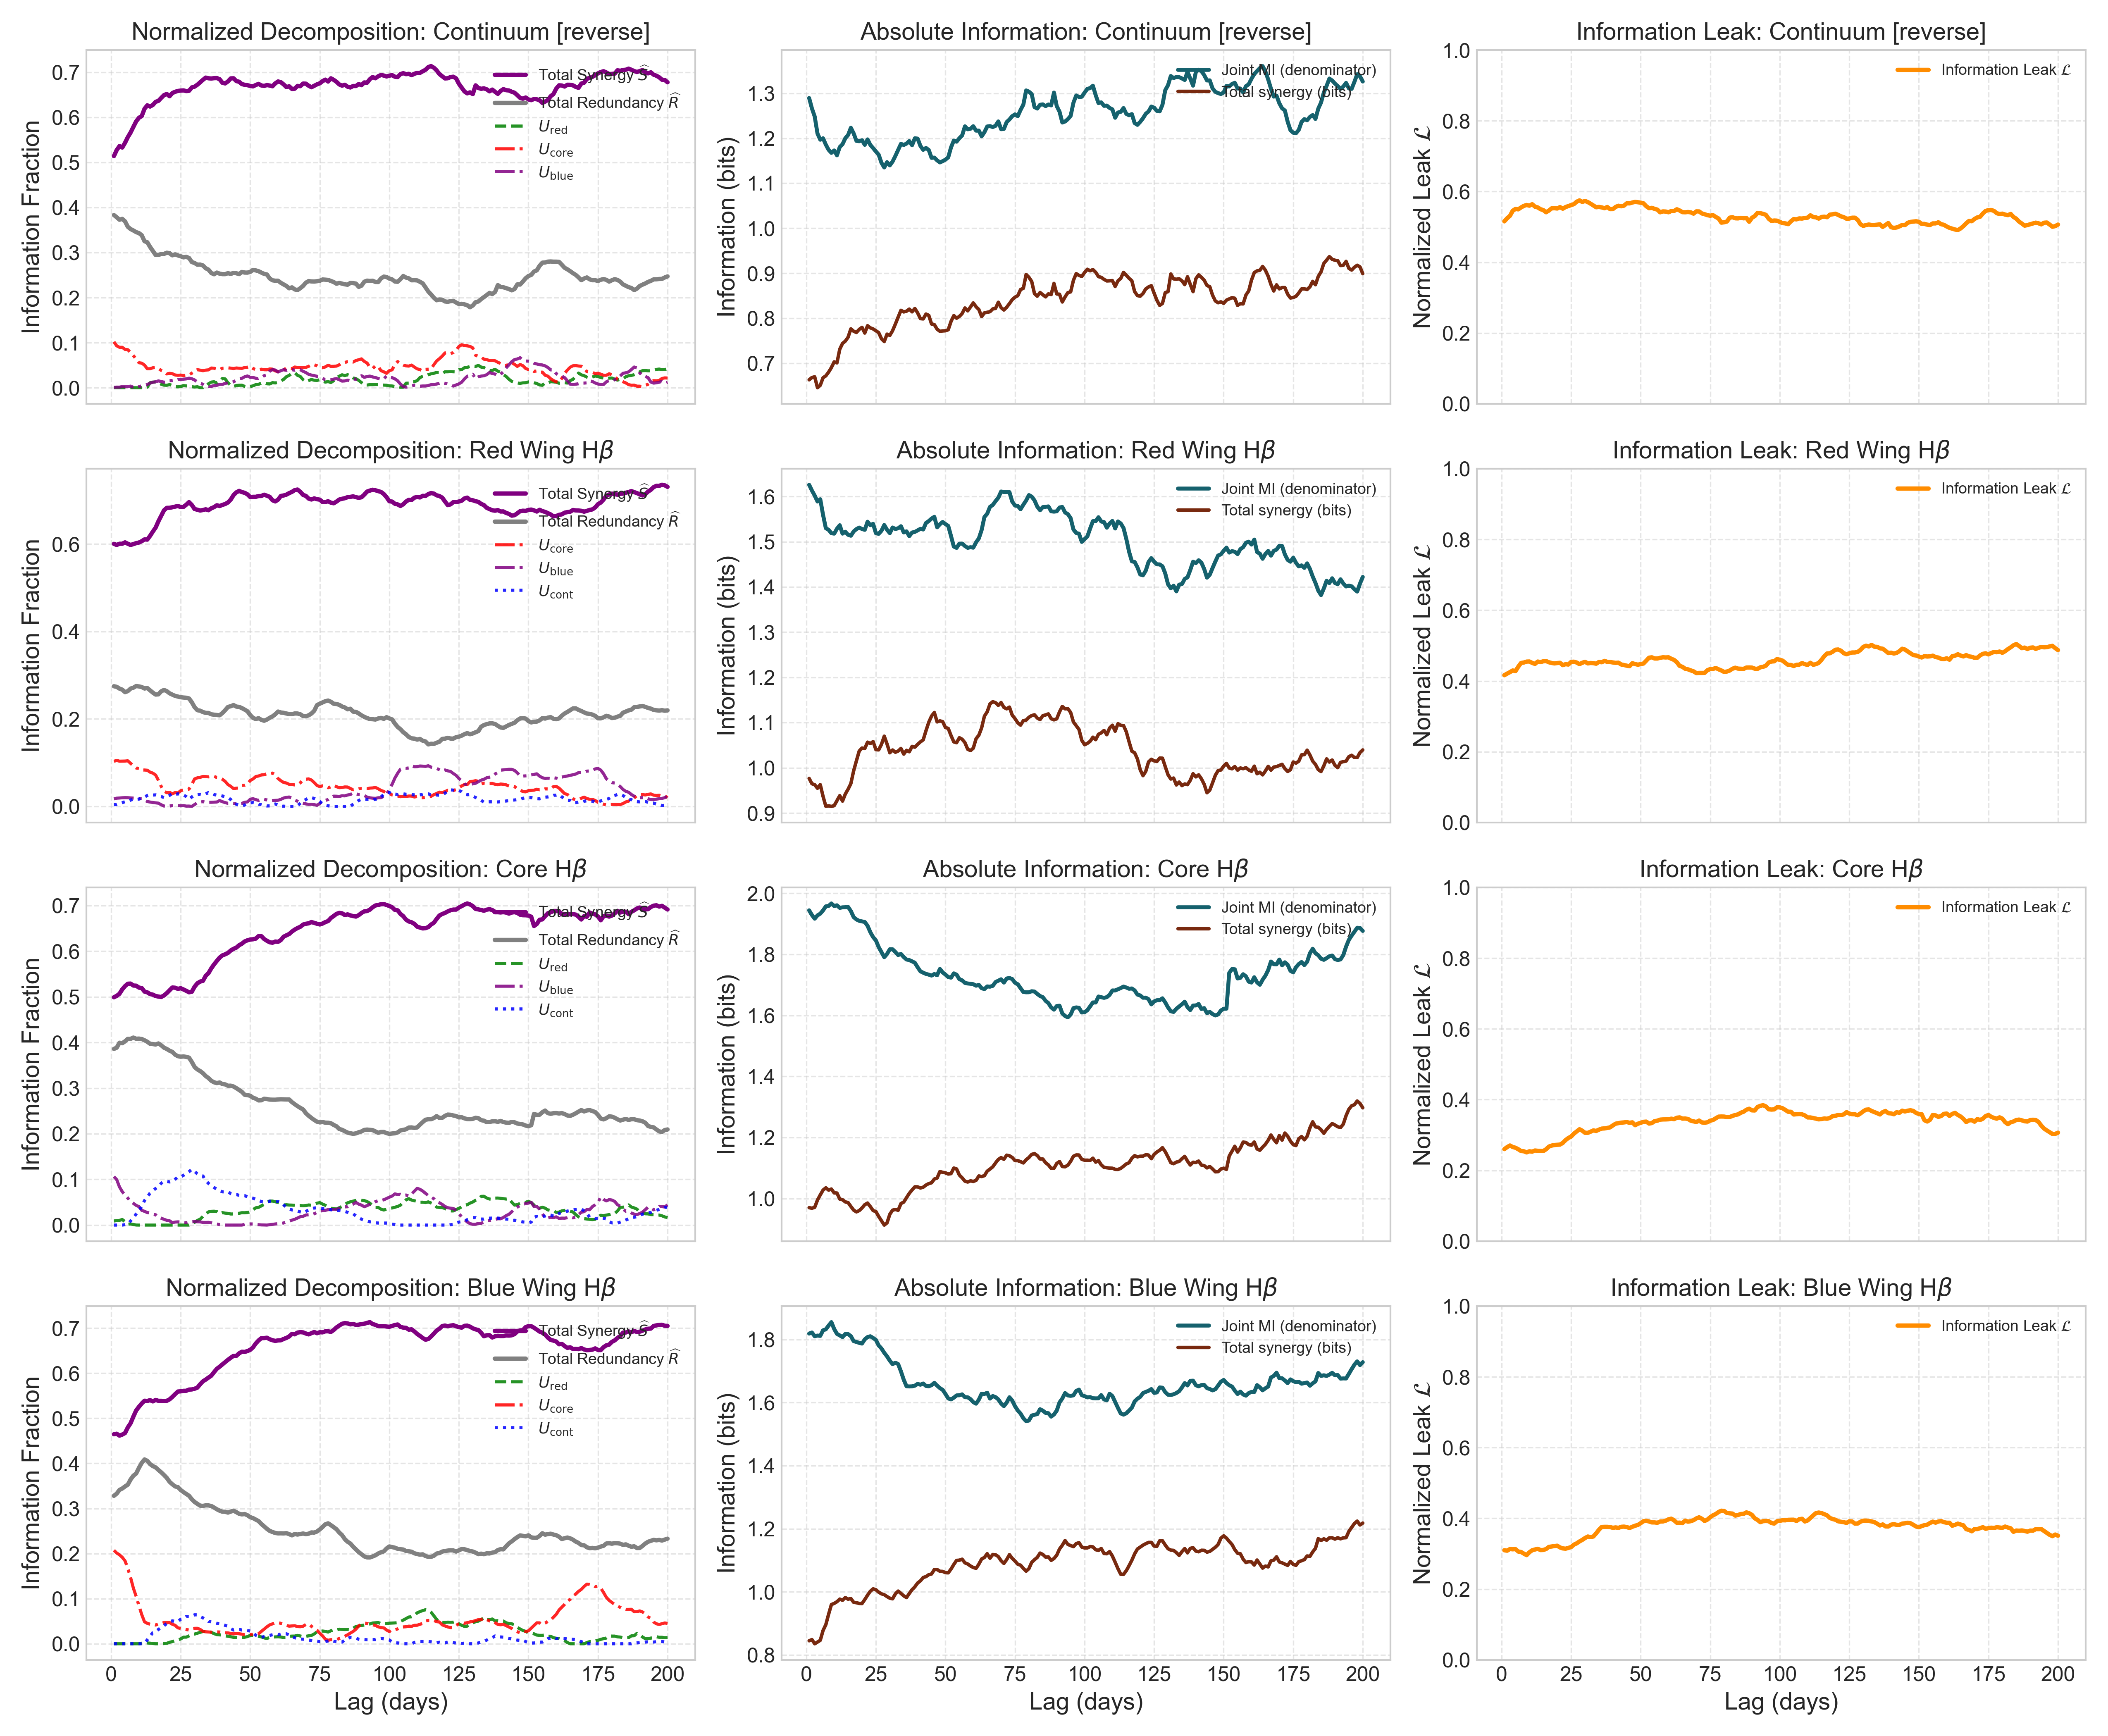
\includegraphics[width=0.95\textwidth]{figure2_surd_lag_scans.png}
\caption{Three-predictor round-robin scans. The left column shows normalized atoms, which sum to unity. The middle column shows total joint mutual information, the normalization denominator, together with absolute total synergy in bits. The right column shows normalized information leak $\mathcal{L}=H(Y\mid X_1,X_2,X_3)/H(Y)$. Total synergy is $S_{12}+S_{13}+S_{23}+S_{123}$, with an analogous sum for redundancy. The continuum-target row is a reverse-prediction estimator diagnostic, not a physical line-to-continuum reverberation model.}
\label{fig:surd_lag_scans}
\end{figure*}

The middle column supplies an important qualification to the normalization argument. The estimated joint mutual information does not approach zero: across targets and lags it spans 1.14--1.97~bits, and at the four normalized maxima it is 1.25--1.66~bits. The corresponding absolute total synergy is 0.90--1.17~bits. Normalization changes the relative shape, especially where joint MI declines, but division by an almost-zero denominator is not an adequate explanation of the real curves. These large absolute values under sparse four-dimensional histograms are themselves estimator-biased, as shown by the matched independent-red-noise control below. We therefore base inference on matched empirical nulls rather than on the height of either curve.

\subsection{Surrogate and Null Hypothesis Testing}

To test the exact primary statistic, we generate 999 null realizations in which all four interpolated series are independently circularly shifted by at least 60~d. Each realization repeats the same three-predictor dimensionality, eight-bin equal-width histogram, strict-overlap sample window, normalization, 1--200~d scan, and maximum statistic used for Figure~\ref{fig:surd_lag_scans}. Circular shifts destroy relative phase alignment while preserving each series' values and cyclic autocorrelation. Figure~\ref{fig:robustness_and_nulls} shows the resulting matched pointwise envelope for the core target and a matched three-predictor bin-count sensitivity test.

Crucially, after applying the Benjamini--Hochberg False Discovery Rate (FDR) correction to the main 3-predictor lag scans over 200 tested lags, \textbf{none of the individual lag bins remains globally significant.} This is the key methodological result: local exceedance above pointwise surrogate envelopes is not sufficient grounds for claiming a physically meaningful delay. Instead, the observed SURD curves should be interpreted as broad lag-dependent structures whose most prominent maxima remain compatible with scanned red-noise nulls once multiple testing is taken seriously.

\begin{figure*}
\centering
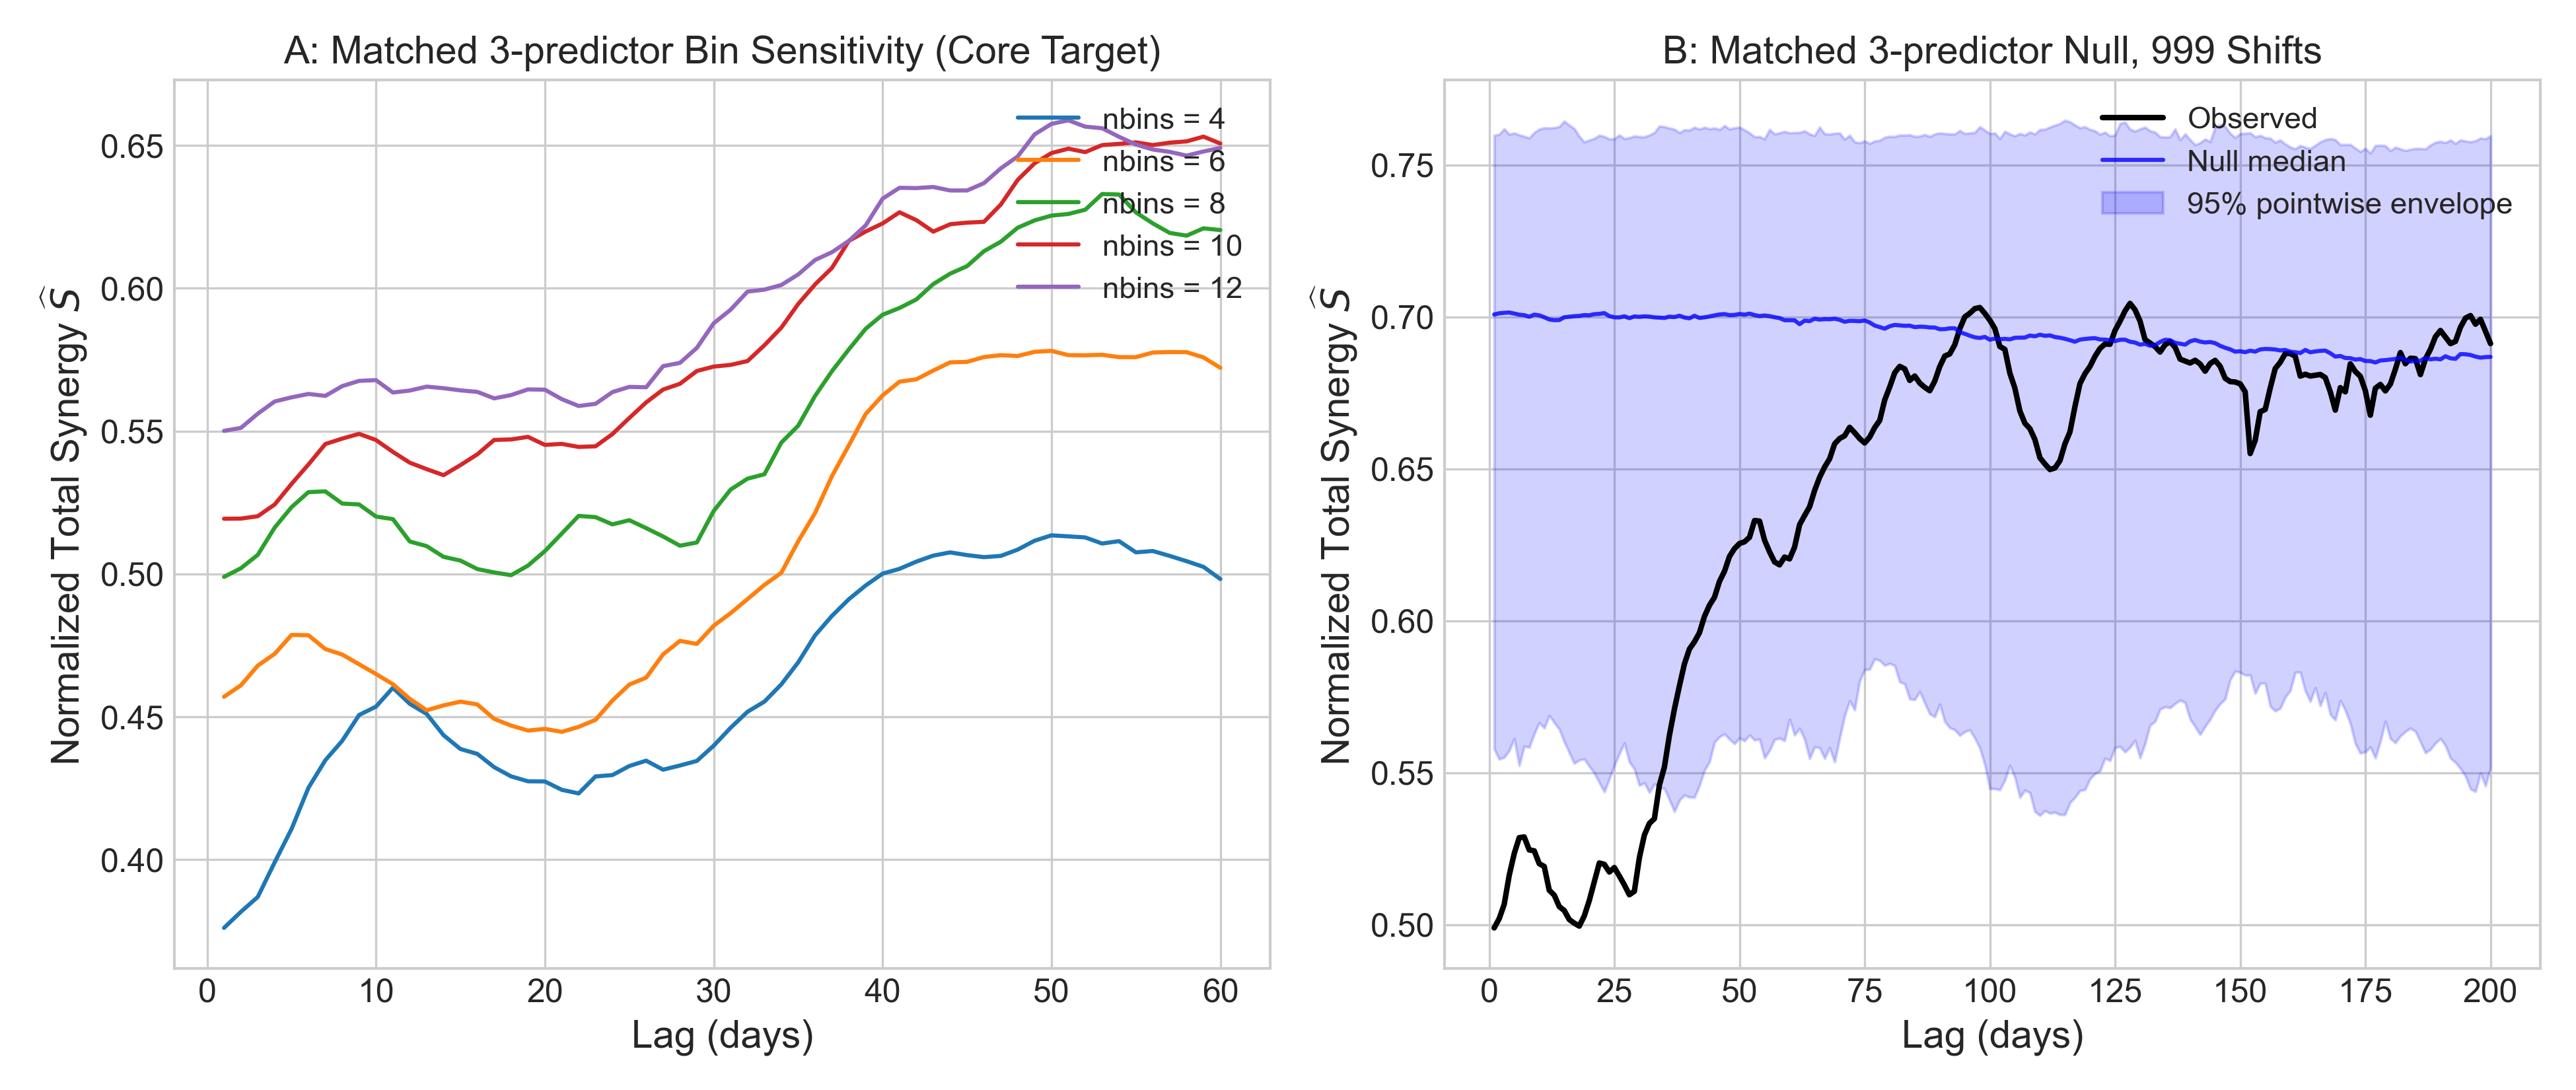
\includegraphics[width=0.95\textwidth]{figure3_robustness_and_nulls.png}
\caption{Matched three-predictor robustness checks for the core target. Panel A varies the equal-width histogram from 4 to 12 bins over 1--60~d. Panel B compares the observed normalized total synergy with the median and pointwise 95\% envelope from 999 circular-shift realizations. The global test uses each realization's maximum over the full 1--200~d scan rather than this pointwise envelope.}
\label{fig:robustness_and_nulls}
\end{figure*}

\subsection{Comparison with Classical Reverberation Lags}

To compare our information-theoretic results with a standard reverberation estimator, we compute the ICCF directly from the native unevenly sampled continuum and line light curves. At each trial lag from $-100$ to $+200$~d in 1-d steps, we linearly interpolate each light curve to the shifted epochs of the other and average the two correlation coefficients. We define the centroid from the contiguous region around the primary peak with $r\geq0.8r_{\max}$ and estimate uncertainties from 5000 flux-randomization/random-subset-sampling (FR/RSS) realizations \citep{WhitePeterson1994,Peterson2004}. Positive lag means that the line follows the continuum.
\begin{table*}
\centering
\begin{tabular}{lcccc}
\hline
\textbf{Target Component} & \textbf{ICCF centroid (d)} & \textbf{ICCF peak (d)} & \textbf{SURD max (d)} & \textbf{Leak min (d)} \\
\hline
Blue Wing H\(\beta\) & $19.44^{+1.52}_{-1.49}$ & 19 & 93 & 9 \\
Core H\(\beta\) & $22.79^{+1.85}_{-1.80}$ & 22 & 128 & 9 \\
Red Wing H\(\beta\) & $30.30^{+4.52}_{-3.62}$ & 15 & 198 & 1 \\
\hline
\end{tabular}
\caption{Native-cadence bidirectional ICCF centroid lags with 16th--84th percentile FR/RSS uncertainties, native ICCF peak lags, and descriptive locations of the normalized three-predictor SURD maximum and leak minimum. The SURD locations are not significant lag measurements.}
\label{tab:iccf_vs_surd}
\end{table*}

The blue-wing and core centroid distributions are compact and prompt. The red-wing ICCF has a native peak at 15~d but a broad above-threshold shoulder, producing a substantially later centroid of $30.30^{+4.52}_{-3.62}$~d. We therefore do not infer velocity-resolved inflow or outflow from these three summaries. In contrast, the normalized three-predictor SURD maxima occur at 93--198~d and fail the matched global null tests. The leak minima are also descriptive diagnostics rather than lag estimates.

\begin{figure*}
\centering
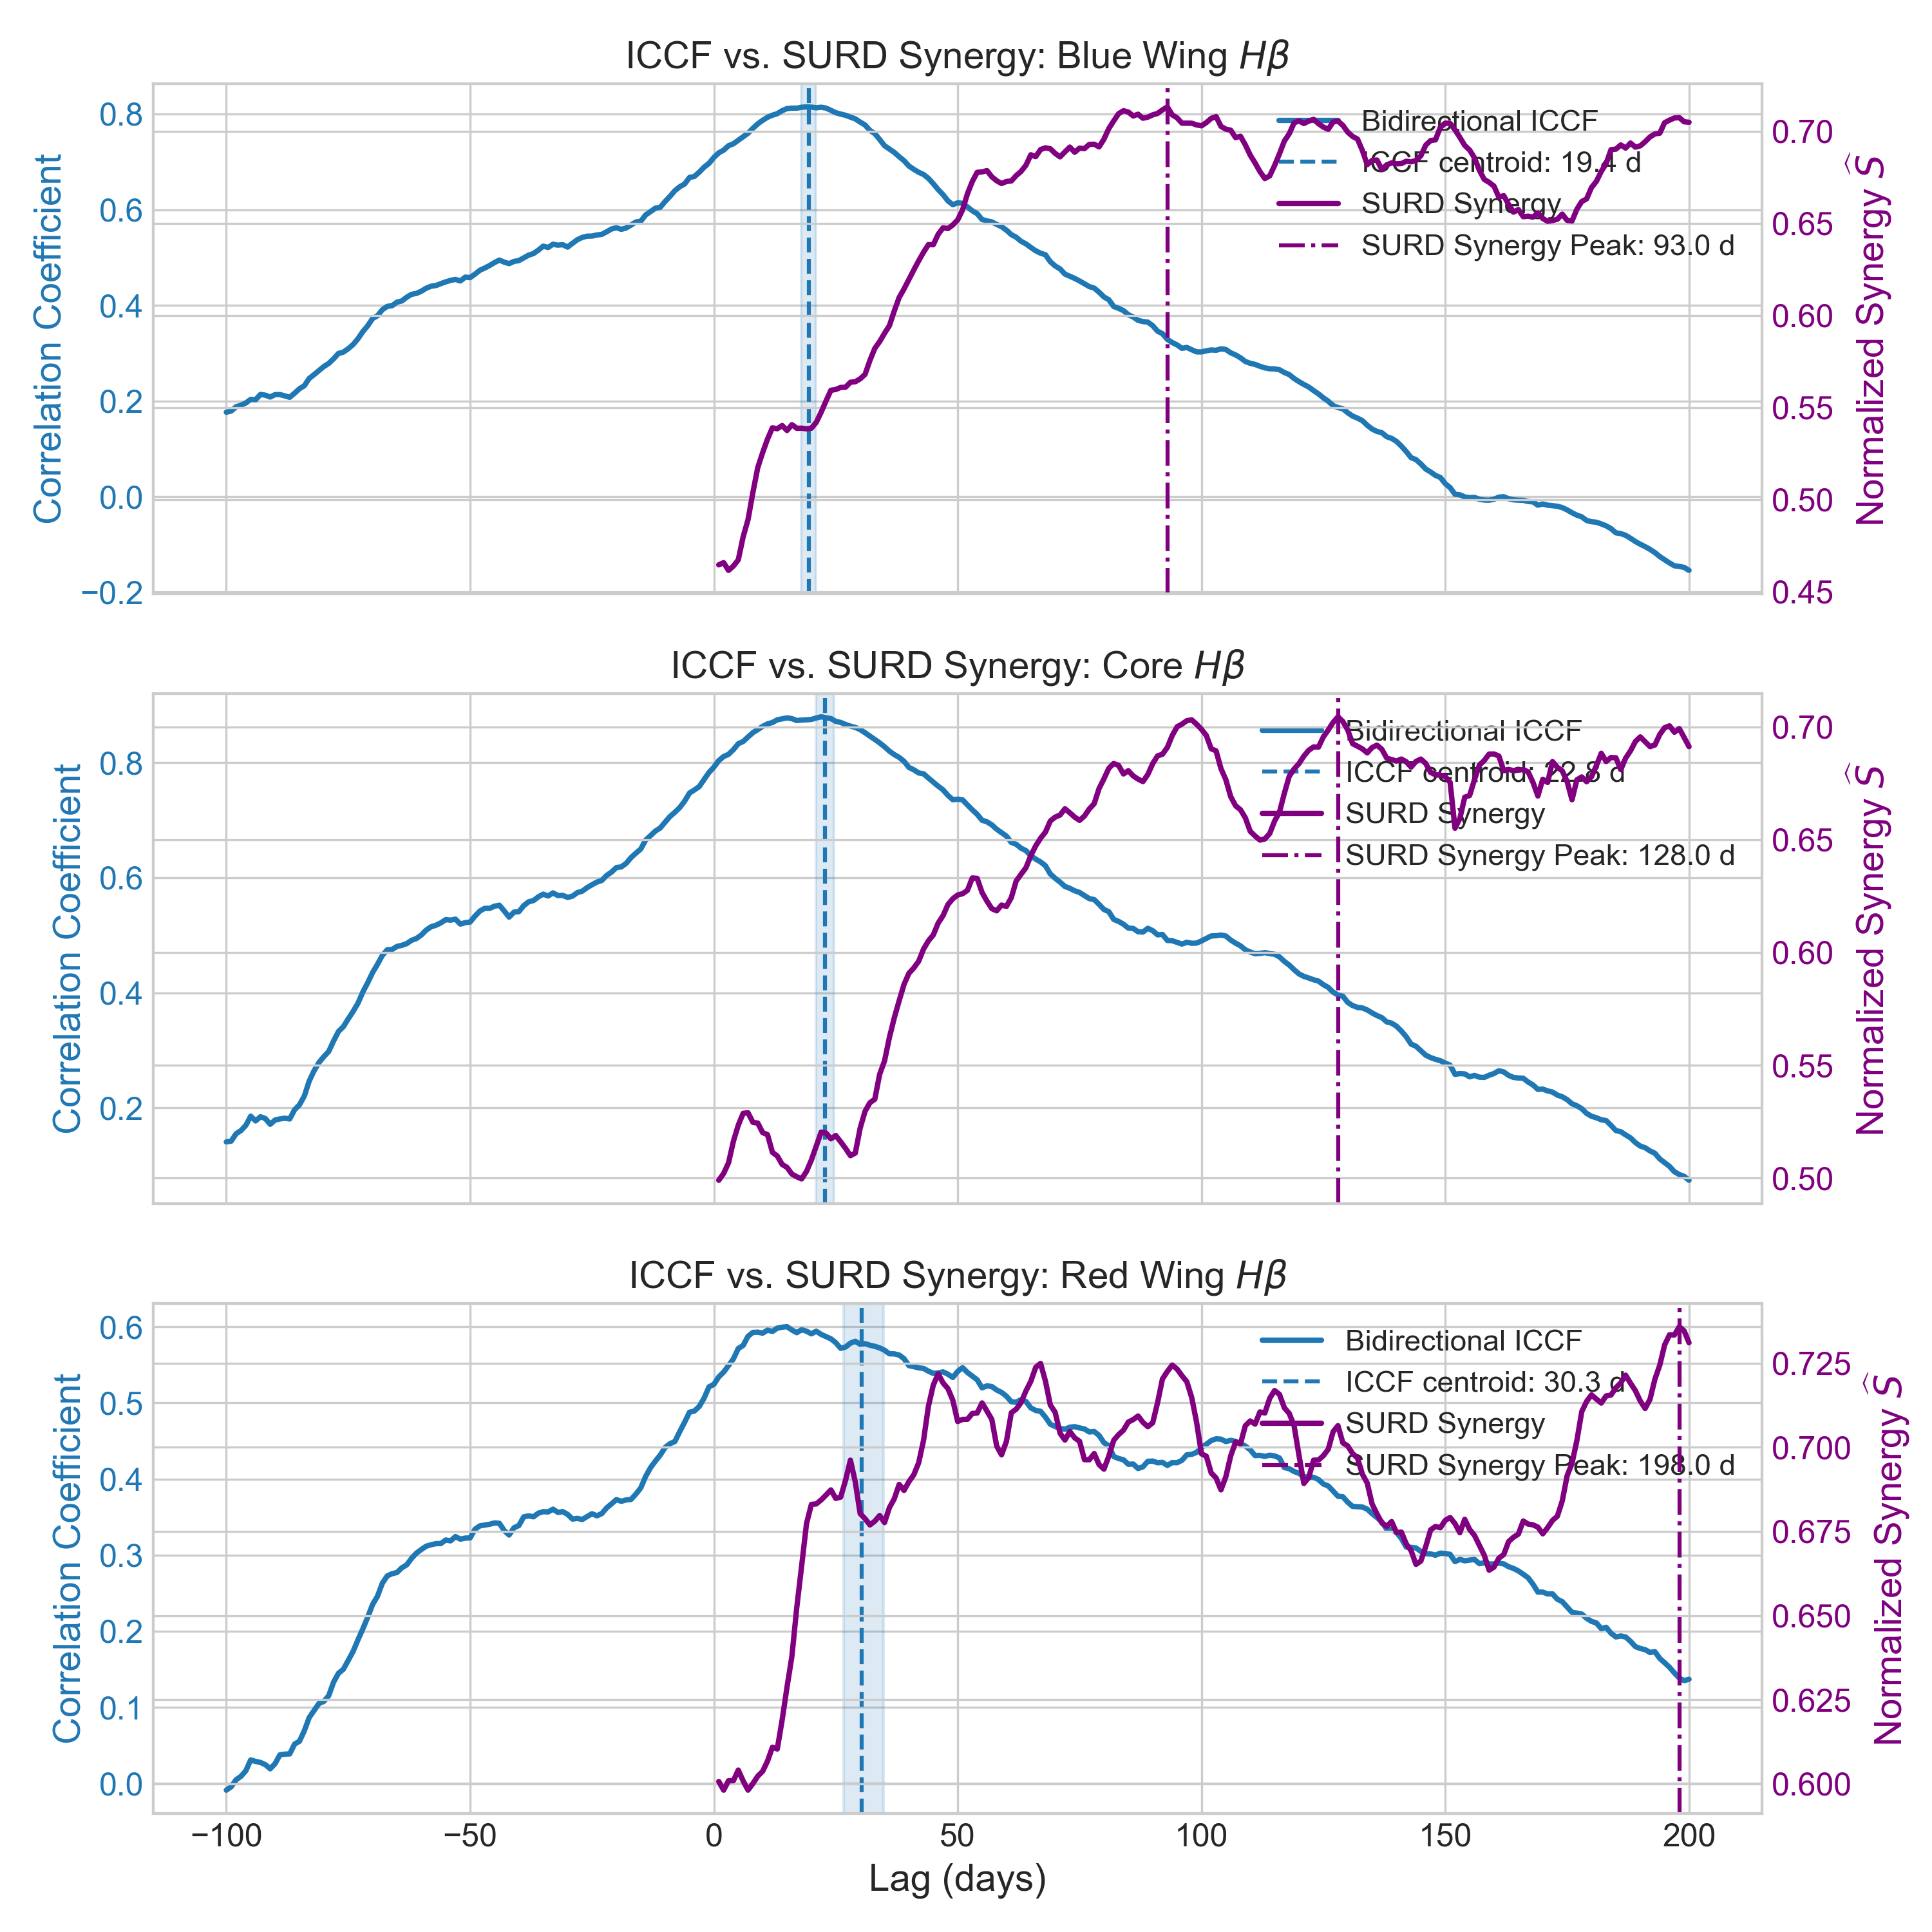
\includegraphics[width=0.95\textwidth]{figure4_iccf_vs_surd.png}
\caption{Native-cadence bidirectional ICCF (blue) and normalized three-predictor SURD total synergy (purple). Blue dashed lines and bands show the FR/RSS centroid median and 16th--84th percentiles; purple dash-dotted lines mark the descriptive SURD maxima. The quantities have different estimands and the SURD maxima are globally non-significant.}
\label{fig:iccf_vs_surd}
\end{figure*}

Figure~\ref{fig:iccf_vs_surd} makes the main contrast visually explicit: pairwise continuum--line correlation peaks remain prompt, whereas the normalized multivariate synergy curve drifts to much longer lags and shows the scan-range dependence documented above. This separation is one of the clearest indications that the long-lag SURD maxima are not tracing the same physical structure as the classical reverberation lag.

\iffalse
\subsection{Stored JAVELIN Chain Behavior}
\label{sec:javelin_comparison}

To supplement the cross-correlation analysis, we inspected previously generated JAVELIN lag chains for the three velocity components \cite{Zu2011}. Unlike the ICCF curves, the archived JAVELIN outputs are not cleanly single-peaked. The blue-wing chain is concentrated near \(\sim 22.5\)~d with a smaller \(\sim 19.5\)~d mode, the core chain is bimodal with strong modes near \(\sim 11.5\) and \(\sim 22.5\)~d, and the red-wing chain is clearly multimodal with substantial probability extending to \(\sim 80\)~d. These features are visible directly in Figure~\ref{fig:javelin_posteriors}.

Because the stored JAVELIN chains do not support a unique, well-behaved single-lag summary under the present configuration, we do not use them as a primary quantitative validation of the ICCF peaks in this draft. Instead, we retain them as a cautionary comparison showing that transfer-function fits can also become alias-prone when the sampling window is difficult.


\begin{figure*}
\centering
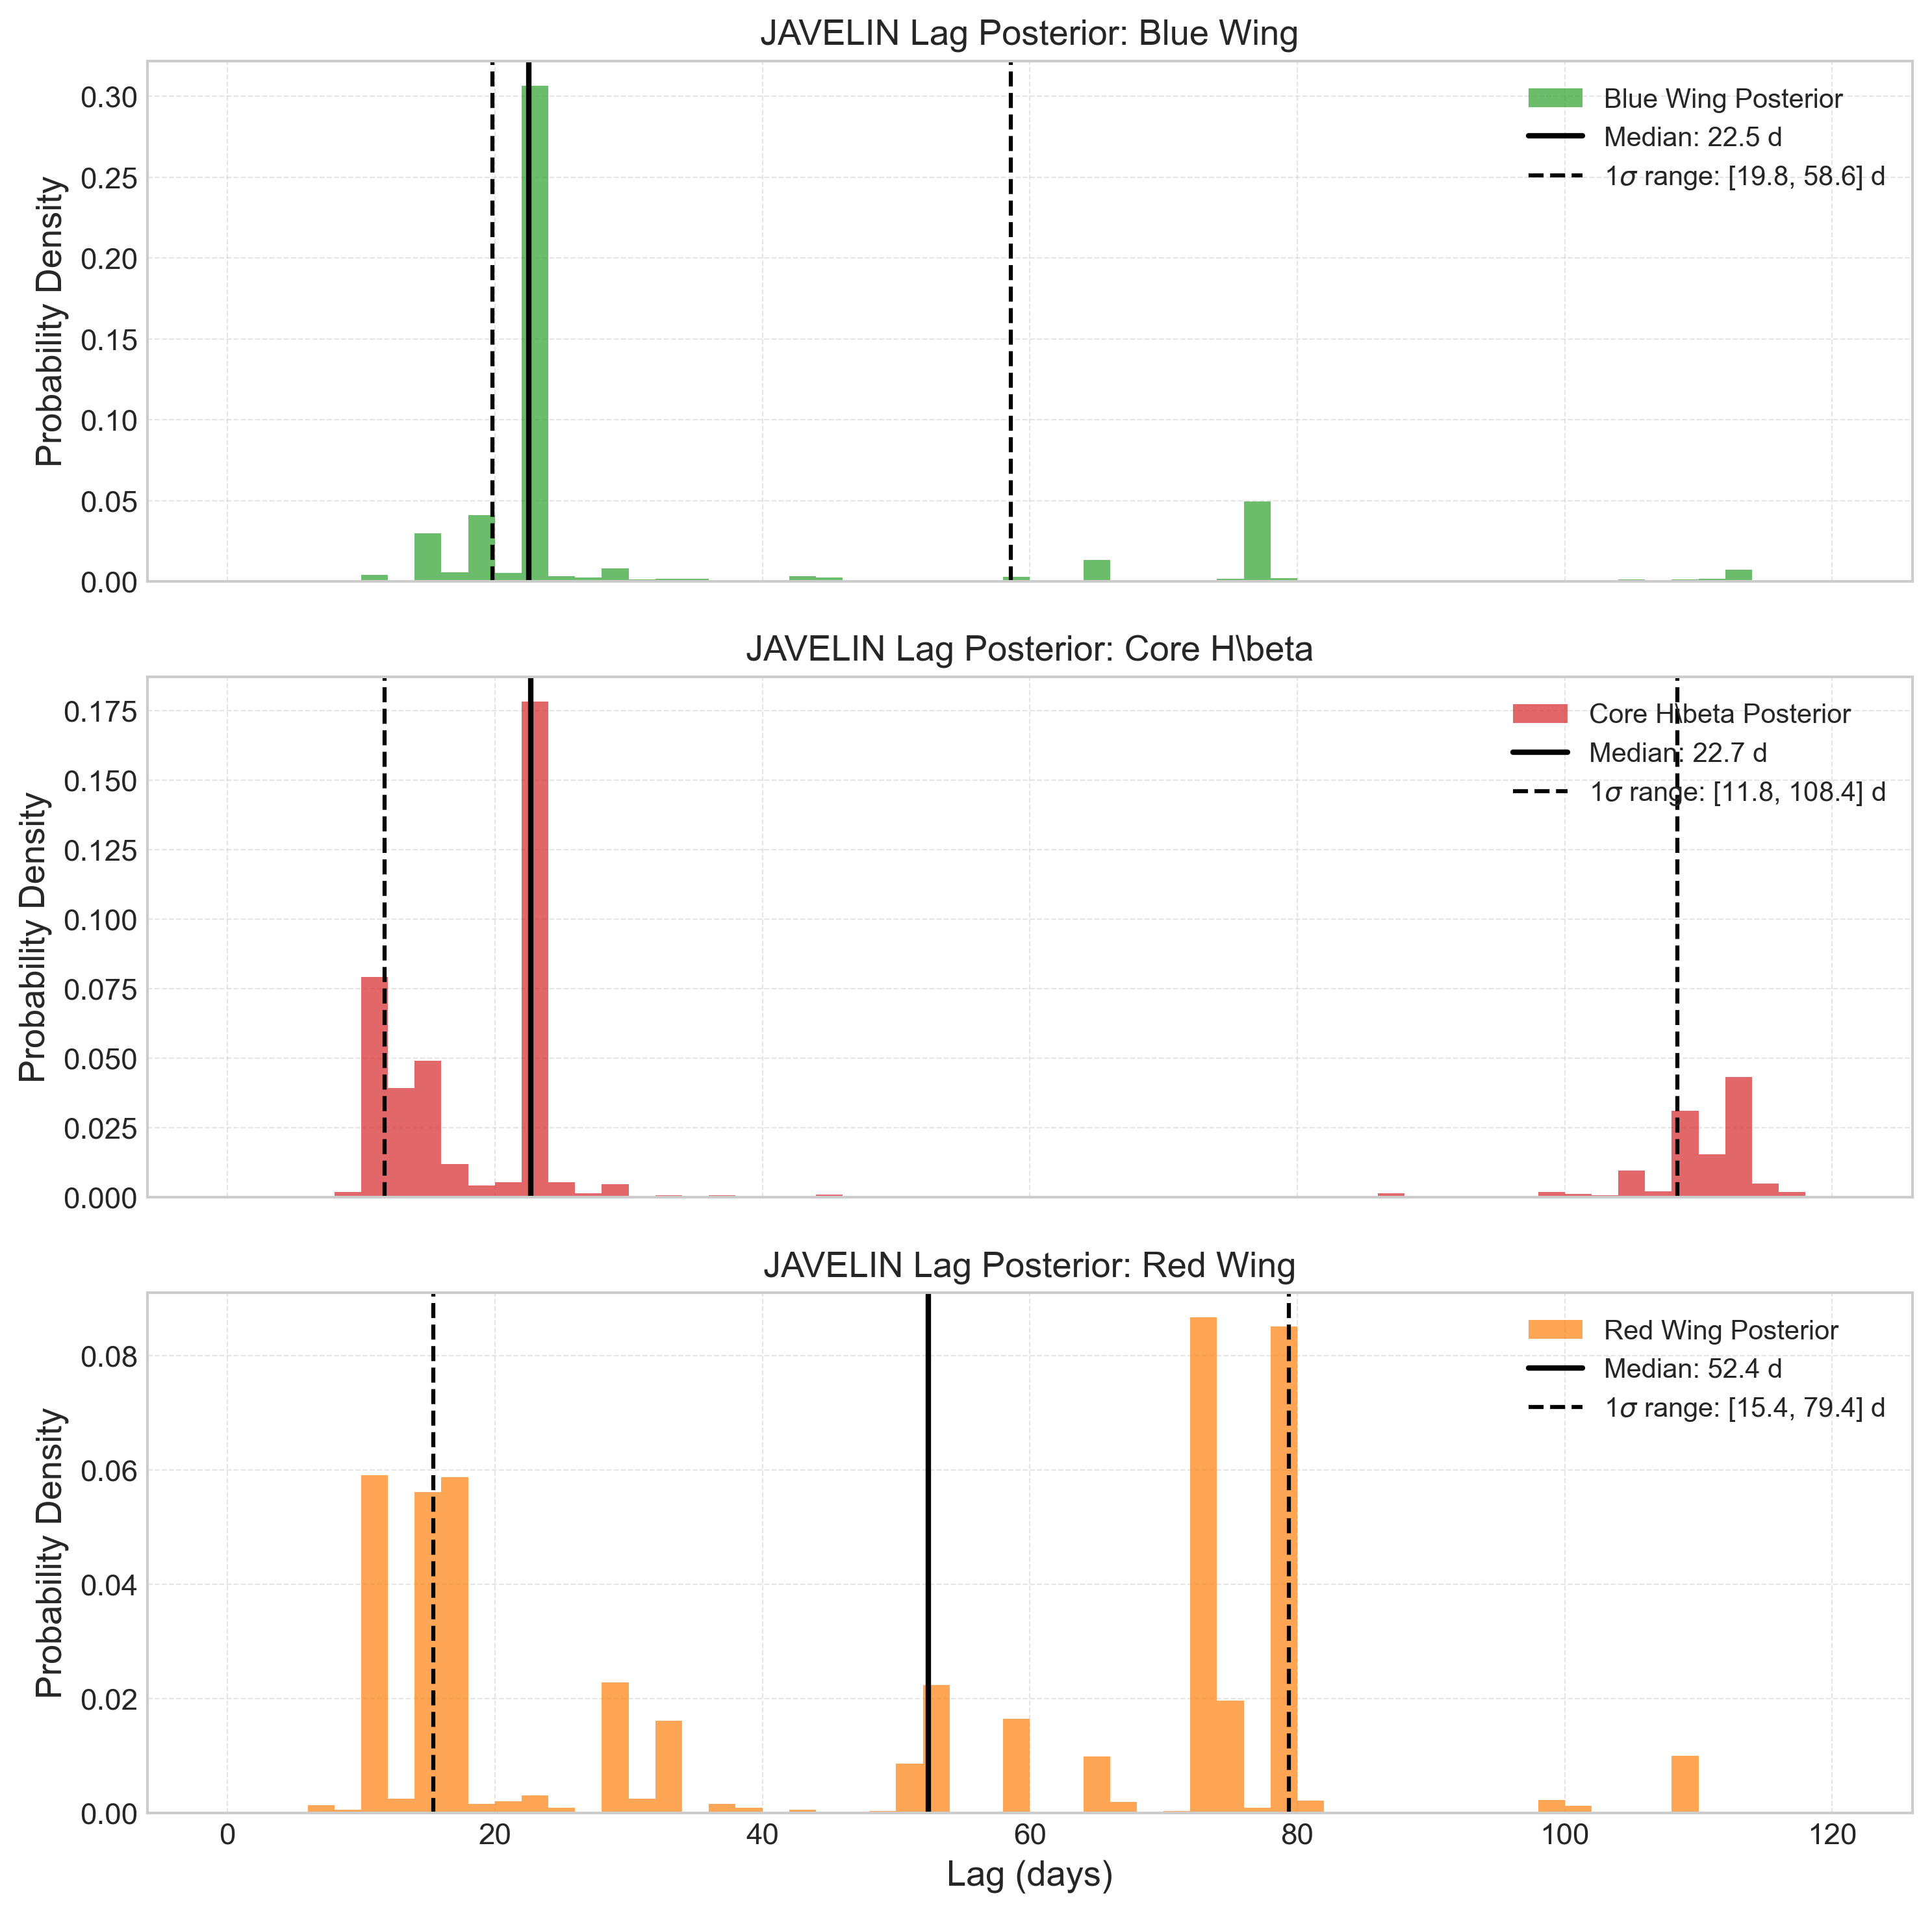
\includegraphics[width=0.8\textwidth]{figure6_javelin_posteriors.png}
\caption{Stored JAVELIN lag-chain histograms for the Blue Wing (top), Core (middle), and Red Wing (bottom) of H\(\beta\) in NGC~5548. The posteriors are visibly multimodal, so they are shown here as qualitative diagnostics rather than decisive single-lag measurements.}
\label{fig:javelin_posteriors}
\end{figure*}

\fi
\subsection{Empirical Multiple-Testing Correction}
\label{sec:dcf_fdr}

For each target and lag, we use the empirical one-sided p-value
\begin{equation}
p(\tau)=\frac{1+\#\{\widehat S_{b}(\tau)\geq\widehat S_{\rm obs}(\tau)\}}{1+B},
\end{equation}
where $B=999$ is the number of matched circular-shift realizations. No distributional approximation is used. Benjamini--Hochberg adjustment across the 200 lags for each target yields no discoveries at $q=0.05$; the smallest unadjusted empirical p-values are 0.694, 0.260, 0.354, and 0.349 for the continuum, red, core, and blue targets, respectively.

To test the selected maximum directly, each of the same 999 realizations contributes its maximum over the full 200-lag scan. The empirical global p-value is
\begin{equation}
p_{\mathrm{global}} = \frac{1 + \#(\widehat{S}_{\mathrm{max, null}} \ge \widehat{S}_{\mathrm{max, real}})}{1 + N_{\mathrm{surrogate}}}.
\end{equation}
The observed maxima are $0.7138$, $0.7358$, $0.7045$, and $0.7133$ for the continuum, red, core, and blue targets. Their global p-values are 1.000, 0.873, 0.947, and 0.936, respectively. The observed maxima are therefore consistent with the scanned red-noise null.

Thus, although local features may appear prominent, none survives the matched scan-wide controls. Empirical multiple-testing corrections and negative controls are necessary before isolated information-curve maxima are interpreted as lags.

\subsection{Continuum-Only Baseline and Prompt Lag Recovery}
\label{sec:continuum_baseline}

The three-predictor round-robin SURD scans in Section~\ref{sec:results} exhibit unconditioned maxima at long lags (93--198~d) that fail empirical global significance tests against circular-shift surrogates ($p_{\mathrm{global}} = 0.873$--$1.000$). A natural question arises: can information-theoretic estimators recover the known physical reverberation delay ($\sim 15$--$25$~d) when the line emission is evaluated directly against the optical continuum driver, without the confounding influence of correlated line predictors?

To test this, we evaluate the one-predictor mutual information baseline:
\begin{equation}
I(Y(t); F_{5100}(t - \tau))
\end{equation}
across lags $\tau \in [0, 200]$~d for the three H\(\beta\) components (Blue Wing, Core, and Red Wing). We evaluate this baseline across all four adopted sampling configurations: daily interpolation, interpolation restricted to gaps $\le 30$~d, within-season interpolation, and native observation pairing.

Under gap-limited sampling (which bridges gaps $\le 30$~d without interpolating across seasonal observing shutdowns), the continuum-only scan identifies prompt mutual information maxima for all three components (Table~\ref{tab:continuum_baseline}):
\begin{itemize}
    \item \textbf{Blue Wing:} $\tau_{\mathrm{peak}} = 16$~d ($I = 0.473$~bits, leak minimum $\mathcal{L} = 0.762$ at 16~d).
    \item \textbf{Line Core:} $\tau_{\mathrm{peak}} = 15$~d ($I = 0.719$~bits, leak minimum $\mathcal{L} = 0.637$ at 15~d).
    \item \textbf{Red Wing:} $\tau_{\mathrm{peak}} = 23$~d ($I = 0.326$~bits, leak minimum $\mathcal{L} = 0.834$ at 23~d).
\end{itemize}
Under within-season sampling, the peak lags and mutual information values are identical to the gap-limited results. Under daily interpolation, the recovered peaks are 20~d (Blue), 16~d (Core), and 13~d (Red). Under native observation pairing, peaks occur at 26~d (Blue), 25~d (Core), and 67~d (Red), although native counts are limited to 61--68 tuples per lag.

\begin{table*}
\centering
\begin{tabular}{lcccccc}
\hline
\textbf{Target Component} & \textbf{Method} & \textbf{Peak Lag (d)} & \textbf{Peak MI (bits)} & \textbf{Null 95\% (bits)} & $\boldsymbol{p}_{\mathbf{global}}$ & \textbf{Leak Minimum (d)} \\
\hline
Blue Wing H\(\beta\) & Gap-limited & 16 & 0.473 & 0.413 & 0.0099 & 16 (0.762) \\
Core H\(\beta\)      & Gap-limited & 15 & 0.719 & 0.489 & 0.0099 & 15 (0.637) \\
Red Wing H\(\beta\)  & Gap-limited & 23 & 0.326 & 0.433 & 0.2178 & 23 (0.834) \\
\hline
Blue Wing H\(\beta\) & Daily       & 20 & 0.446 & --    & --     & 20 (0.776) \\
Core H\(\beta\)      & Daily       & 16 & 0.660 & --    & --     & 16 (0.660) \\
Red Wing H\(\beta\)  & Daily       & 13 & 0.265 & --    & --     & 13 (0.867) \\
\hline
\end{tabular}
\caption{One-predictor continuum baseline lag recovery and significance calibration across 201 lags ($0$--$200$~d). Statistical significance is evaluated against $N=100$ circular-shift surrogates of the 5100~\AA\ continuum. Prompt peaks for the Blue Wing (16~d) and Line Core (15~d) are globally significant ($p_{\mathrm{global}} < 0.01$), while the Red Wing peak (23~d) lies within the 95th percentile null envelope.}
\label{tab:continuum_baseline}
\end{table*}

We calibrate statistical significance using $N=100$ circular-shift null realizations of the continuum light curve, evaluating the scan-wide maximum-statistic distribution. Crucially, the prompt peaks for the Blue Wing ($16$~d) and Line Core ($15$~d) are \textbf{globally statistically significant} ($p_{\mathrm{global}} = 0.0099$, $p < 0.01$). In contrast, the Red Wing peak ($23$~d) falls within the 95th percentile null maximum ($0.433$~bits, $p_{\mathrm{global}} = 0.218$), consistent with its broader cross-correlation profile.

In synthetic simulations with an injected 20-day delay, the one-predictor continuum baseline cleanly recovers the true delay ($17$--$22$~d) across all four random seeds and all sampling methods. This establishes a key methodological insight: mutual information is fully capable of resolving prompt reverberation delays, but the unconditioned three-predictor SURD setup suffers from inter-line cross-correlations that create spurious long-lag maxima when line components are used as predictors of one another.

\subsection{Calibration of False Positives and Detection Power}
\label{sec:detection_power}

A rigorous application of information theory to observational astronomical data requires determining the detection threshold and false positive rate under realistic campaign conditions. To quantify the sensitivity limits of the 1988--1993 NGC~5548 observing window, we conduct a controlled simulation grid across response amplitudes and delays.

We simulate synthetic Damped Random Walk (DRW) continuum drivers ($\tau_{\mathrm{DRW}} = 50.0$~d) and generate delayed line responses:
\begin{equation}
y(t) = A \cdot \bar{x}_{\mathrm{delayed}}(t) + (1 - A) \cdot \eta_{\mathrm{indep}}(t),
\end{equation}
where $A \in [0.0, 1.0]$ is the coherent response amplitude, $\bar{x}_{\mathrm{delayed}}(t)$ is the continuum driver convolved with a top-hat transfer function of width 5~d centered at delay $\tau_{\mathrm{true}}$, and $\eta_{\mathrm{indep}}(t)$ is an independent red-noise process representing autonomous line variability. The simulated signals are sampled at the exact 224 spectroscopic dates and 557 continuum dates of the adopted NGC~5548 dataset, with Gaussian noise added according to observed photometric uncertainties. We evaluate a parameter grid spanning response amplitudes $A \in \{0.0, 0.2, 0.4, 0.6, 0.8, 1.0\}$ and true delays $\tau_{\mathrm{true}} \in \{10, 20, 30\}$~d, executing $N=50$ independent Monte Carlo realizations per cell (800 total realizations).

\begin{table*}
\centering
\begin{tabular}{ccccccc}
\hline
\textbf{Amplitude} $A$ & \textbf{True Lag $\tau$ (d)} & \textbf{Detection Power} & \textbf{Recovery $\le 3$~d} & \textbf{Lag Bias (d)} & \textbf{Lag RMSE (d)} & \textbf{Mean Peak MI (bits)} \\
\hline
0.0 (Null) & -- & 0.06 & -- & -- & -- & 0.111 \\
\hline
0.2 & 10 & 0.02 & 0.08 & $+24.46$ & 31.11 & 0.127 \\
0.2 & 20 & 0.02 & 0.18 & $+10.46$ & 23.67 & 0.123 \\
0.2 & 30 & 0.08 & 0.16 & $+4.78$  & 19.31 & 0.149 \\
\hline
0.4 & 10 & 0.44 & 0.68 & $+5.86$  & 16.27 & 0.223 \\
0.4 & 20 & 0.36 & 0.54 & $+1.74$  & 10.61 & 0.234 \\
0.4 & 30 & 0.38 & 0.58 & $+2.46$  & 10.81 & 0.264 \\
\hline
0.6 & 10 & 0.96 & 0.96 & $+0.00$  & 1.40  & 0.502 \\
0.6 & 20 & 0.96 & 0.96 & $+0.38$  & 1.75  & 0.527 \\
0.6 & 30 & 0.96 & 0.96 & $-0.04$  & 1.54  & 0.513 \\
\hline
0.8 & 10 & 1.00 & 1.00 & $+0.12$  & 0.92  & 0.873 \\
0.8 & 20 & 1.00 & 1.00 & $+0.00$  & 1.10  & 0.904 \\
0.8 & 30 & 1.00 & 1.00 & $-0.02$  & 0.97  & 0.884 \\
\hline
1.0 & 10 & 1.00 & 1.00 & $+0.06$  & 0.71  & 1.027 \\
1.0 & 20 & 1.00 & 1.00 & $-0.08$  & 0.87  & 1.024 \\
1.0 & 30 & 1.00 & 1.00 & $-0.26$  & 0.84  & 1.025 \\
\hline
\end{tabular}
\caption{Detection power, false positive calibration, and lag recovery error across an amplitude-delay grid ($N=50$ realizations per cell). Detection is defined as recovery within $\pm 3$~d of the true delay with peak MI exceeding the empirical 95\% null threshold ($0.1902$~bits). The empirical false positive rate under the null ($A=0.0$) is $0.06$.}
\label{tab:detection_power}
\end{table*}

\begin{figure*}
\centering
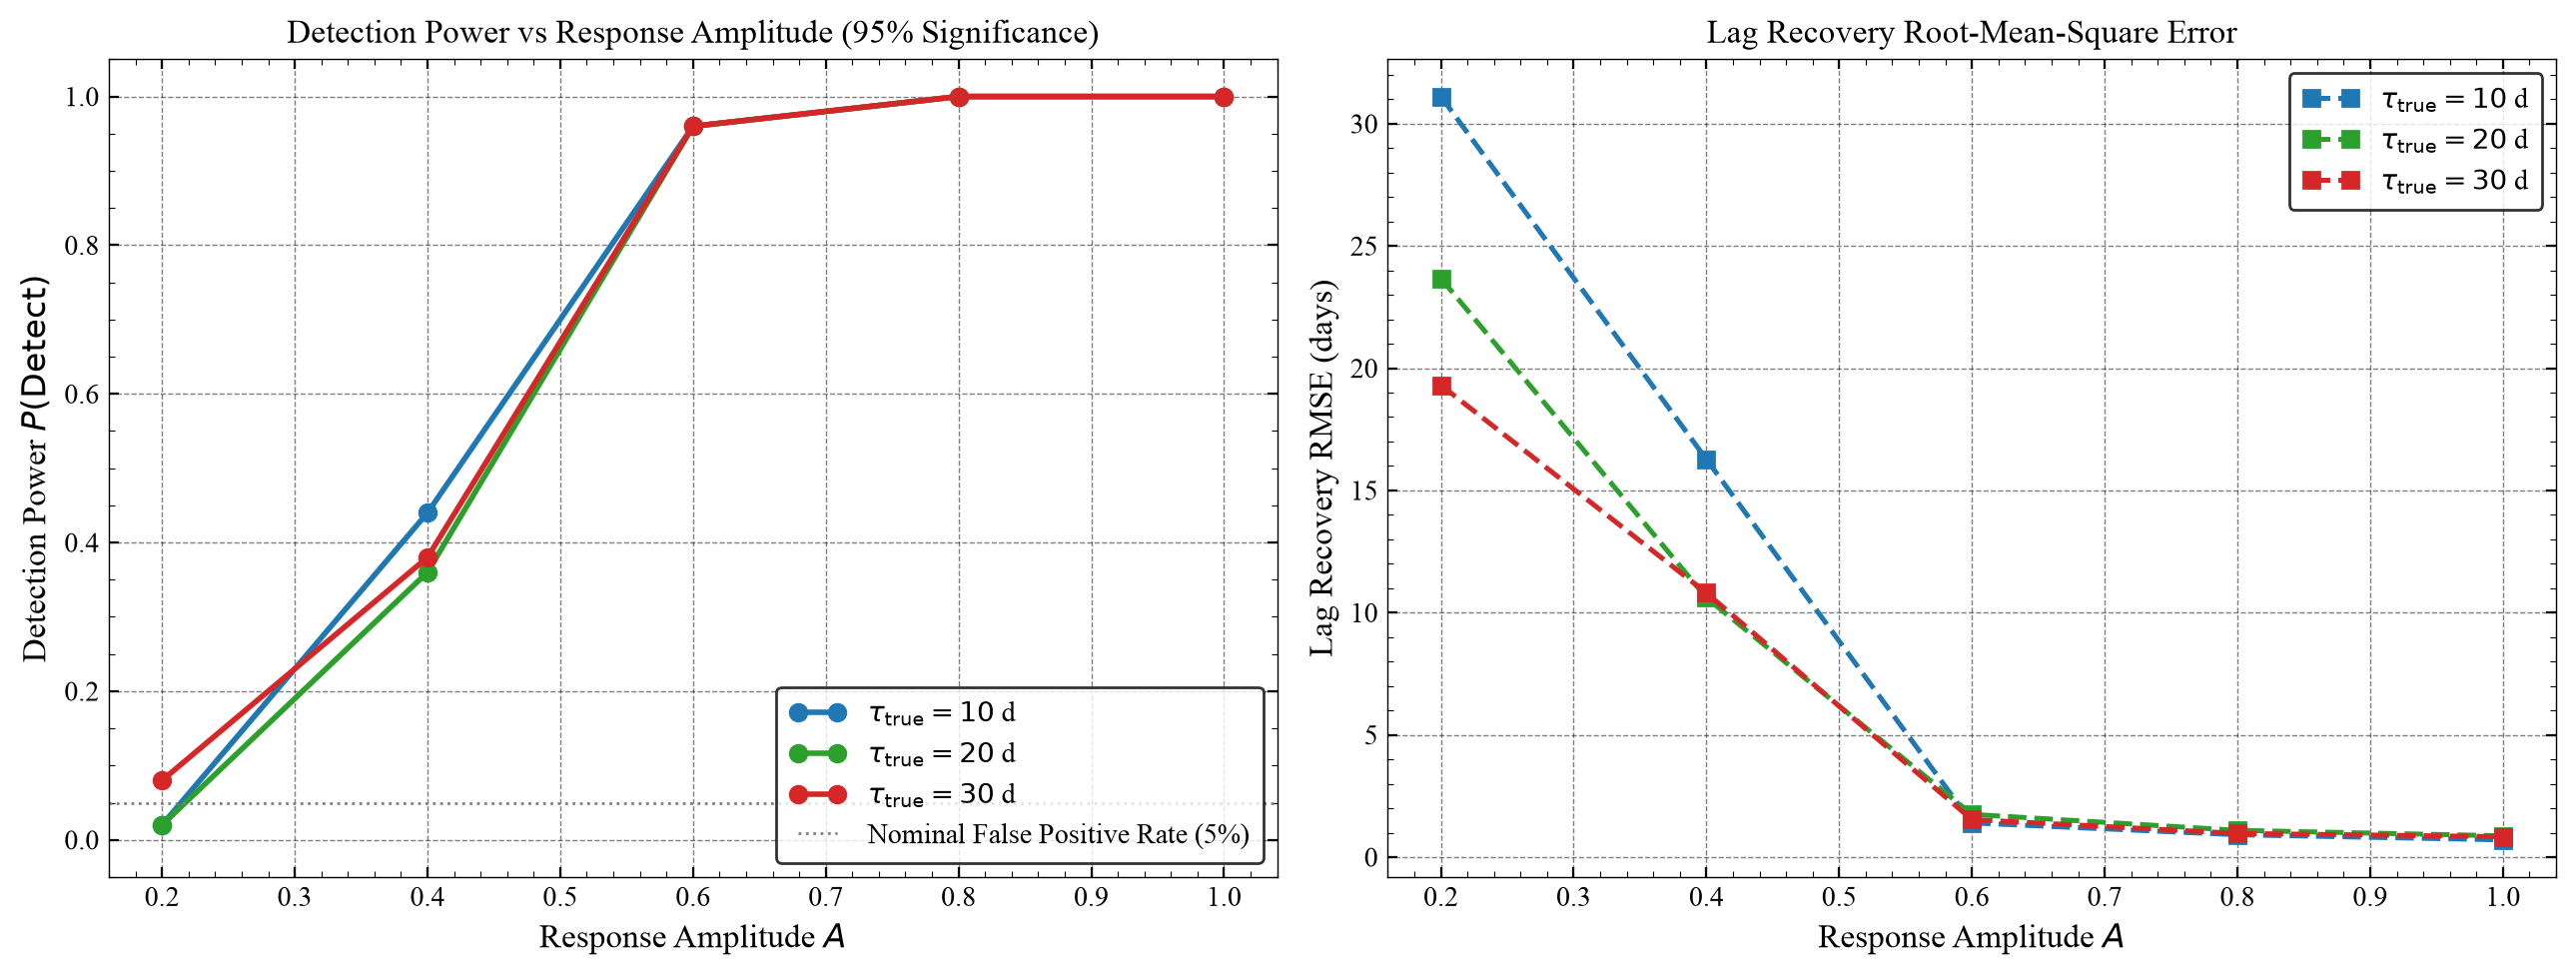
\includegraphics[width=0.95\textwidth]{figure12_detection_power.png}
\caption{Detection power (left) and lag recovery root-mean-square error (right) as a function of response amplitude $A$ across delays $\tau_{\mathrm{true}} \in \{10, 20, 30\}$~d. Dotted horizontal line marks the nominal 5\% false positive rate under the null ($A=0.0$). A coherent response amplitude $A \ge 0.5$--$0.6$ is required to achieve $\ge 90\%$ detection power and lag RMSE $< 2.0$~d under the NGC~5548 observing cadence.}
\label{fig:detection_power}
\end{figure*}

Under the pure null hypothesis ($A = 0.0$, where line variability is completely independent of the continuum), the empirical 95th percentile of the scan-wide maximum MI is $0.1902$~bits. The empirical false positive rate at this decision threshold is $\mathrm{FPR} = 0.06$ (3 of 50 realizations exceed the threshold), in excellent agreement with the nominal 5\% design level.

Table~\ref{tab:detection_power} and Figure~\ref{fig:detection_power} reveal a sharp detection boundary:
\begin{enumerate}
    \item \textbf{Sub-threshold Regime ($A \le 0.2$):} Detection power is negligible ($2\%$--$8\%$), and lag RMSE is large ($19$--$31$~d). The recovered peaks are scattered uniformly across the scan window by sample noise and interpolation trends.
    \item \textbf{Intermediate Transition ($A = 0.4$):} Detection power rises to $36\%$--$44\%$, with $54\%$--$68\%$ of realizations locating the lag within $\pm 3$~d. Lag RMSE drops to $10$--$16$~d.
    \item \textbf{High-Confidence Recovery ($A \ge 0.6$):} Detection power reaches $96\%$ across all tested delays. The true delay is recovered within $\pm 3$~d in $96\%$ of realizations, lag bias is negligible ($-0.04$ to $+0.38$~d), and lag RMSE is only $1.4$--$1.7$~d.
    \item \textbf{Asymptotic Precision ($A \ge 0.8$):} Detection power reaches $100\%$, with lag RMSE $< 1.1$~d and mean peak mutual information exceeding $0.87$~bits.
\end{enumerate}
This benchmark defines the observational sensitivity envelope for NGC~5548: a physical reverberation response must contribute at least $50\%$--$60\%$ of the total line variance ($A \gtrsim 0.5$--$0.6$) to be reliably detected ($> 90\%$ power) and positioned within $\pm 2$~d.

\subsection{Testing Incremental Velocity Information and Kinematic Coupling}
\label{sec:incremental_information}

In velocity-resolved reverberation mapping, an essential astrophysical question is whether different line components drive or predict one another---for example, whether the high-velocity wings transfer gas into the low-velocity core, or whether an asymmetric outflow/inflow creates a directional lag between the blue and red wings \citep{Xi2025}. In an information-theoretic framework, this requires testing whether a candidate velocity component $X_{\mathrm{wing}}(t)$ provides \textit{incremental predictive information} about another component $Y(t+\tau)$ after conditioning on both the driving continuum $F_{5100}(t)$ and the target's own red-noise history $Y(t)$:
\begin{equation}
H_0: \quad I(Y(t+\tau); X_{\mathrm{wing}}(t) \mid F_{5100}(t), Y(t)) = 0.
\end{equation}
If $H_0$ holds, the observed correlations between velocity components are fully explained by their common response to the central continuum driver and their intrinsic temporal autocorrelation, leaving no evidence for directional kinematic transport.

\begin{table*}
\centering
\begin{tabular}{llccccc}
\hline
\textbf{Target} $Y$ & \textbf{Candidate Wing} $X_{\mathrm{wing}}$ & \textbf{Peak Lag (d)} & \textbf{Peak CMI (bits)} & \textbf{Null 95\% (bits)} & $\boldsymbol{p}_{\mathbf{global}}$ & $\boldsymbol{\Delta R^2_{\mathrm{held\text{-}out}}}$ \\
\hline
Core H\(\beta\)     & Blue Wing (discrete)   & 96 & 0.218 & 0.419 & 0.903 & $+0.017$ \\
Core H\(\beta\)     & Blue Wing (KNN $k=5$)   & 58 & 0.164 & 0.500 & 1.000 & -- \\
Core H\(\beta\)     & Red Wing (discrete)    & 100 & 0.192 & 0.360 & 1.000 & $-0.213$ \\
Core H\(\beta\)     & Red Wing (KNN $k=5$)    & 91 & 0.213 & 0.384 & 0.968 & -- \\
Red Wing H\(\beta\)  & Blue Wing (Outflow, discrete) & 39 & 0.211 & 0.345 & 0.903 & -- \\
Red Wing H\(\beta\)  & Blue Wing (Outflow, KNN)      & 30 & 0.271 & 0.351 & 0.677 & -- \\
Blue Wing H\(\beta\) & Red Wing (Inflow, discrete)  & 34 & 0.253 & 0.409 & 0.968 & $-0.053$ \\
Blue Wing H\(\beta\) & Red Wing (Inflow, KNN)       & 97 & 0.349 & 0.453 & 0.613 & -- \\
\hline
\end{tabular}
\caption{Tests of incremental predictive information conditioned on the continuum driver $F_{5100}(t)$ and target history $Y(t)$. Global empirical $p$-values are evaluated against 30 circular-shift surrogates that strictly preserve the $(Y(t+\tau), F_{5100}(t), Y(t))$ distribution while randomizing $X_{\mathrm{wing}}$. Out-of-sample $\Delta R^2_{\mathrm{held\text{-}out}}$ represents the change in predictive variance on held-out observing seasons. None of the directional kinematic hypotheses survives conditioning.}
\label{tab:incremental_information}
\end{table*}

\begin{figure*}
\centering
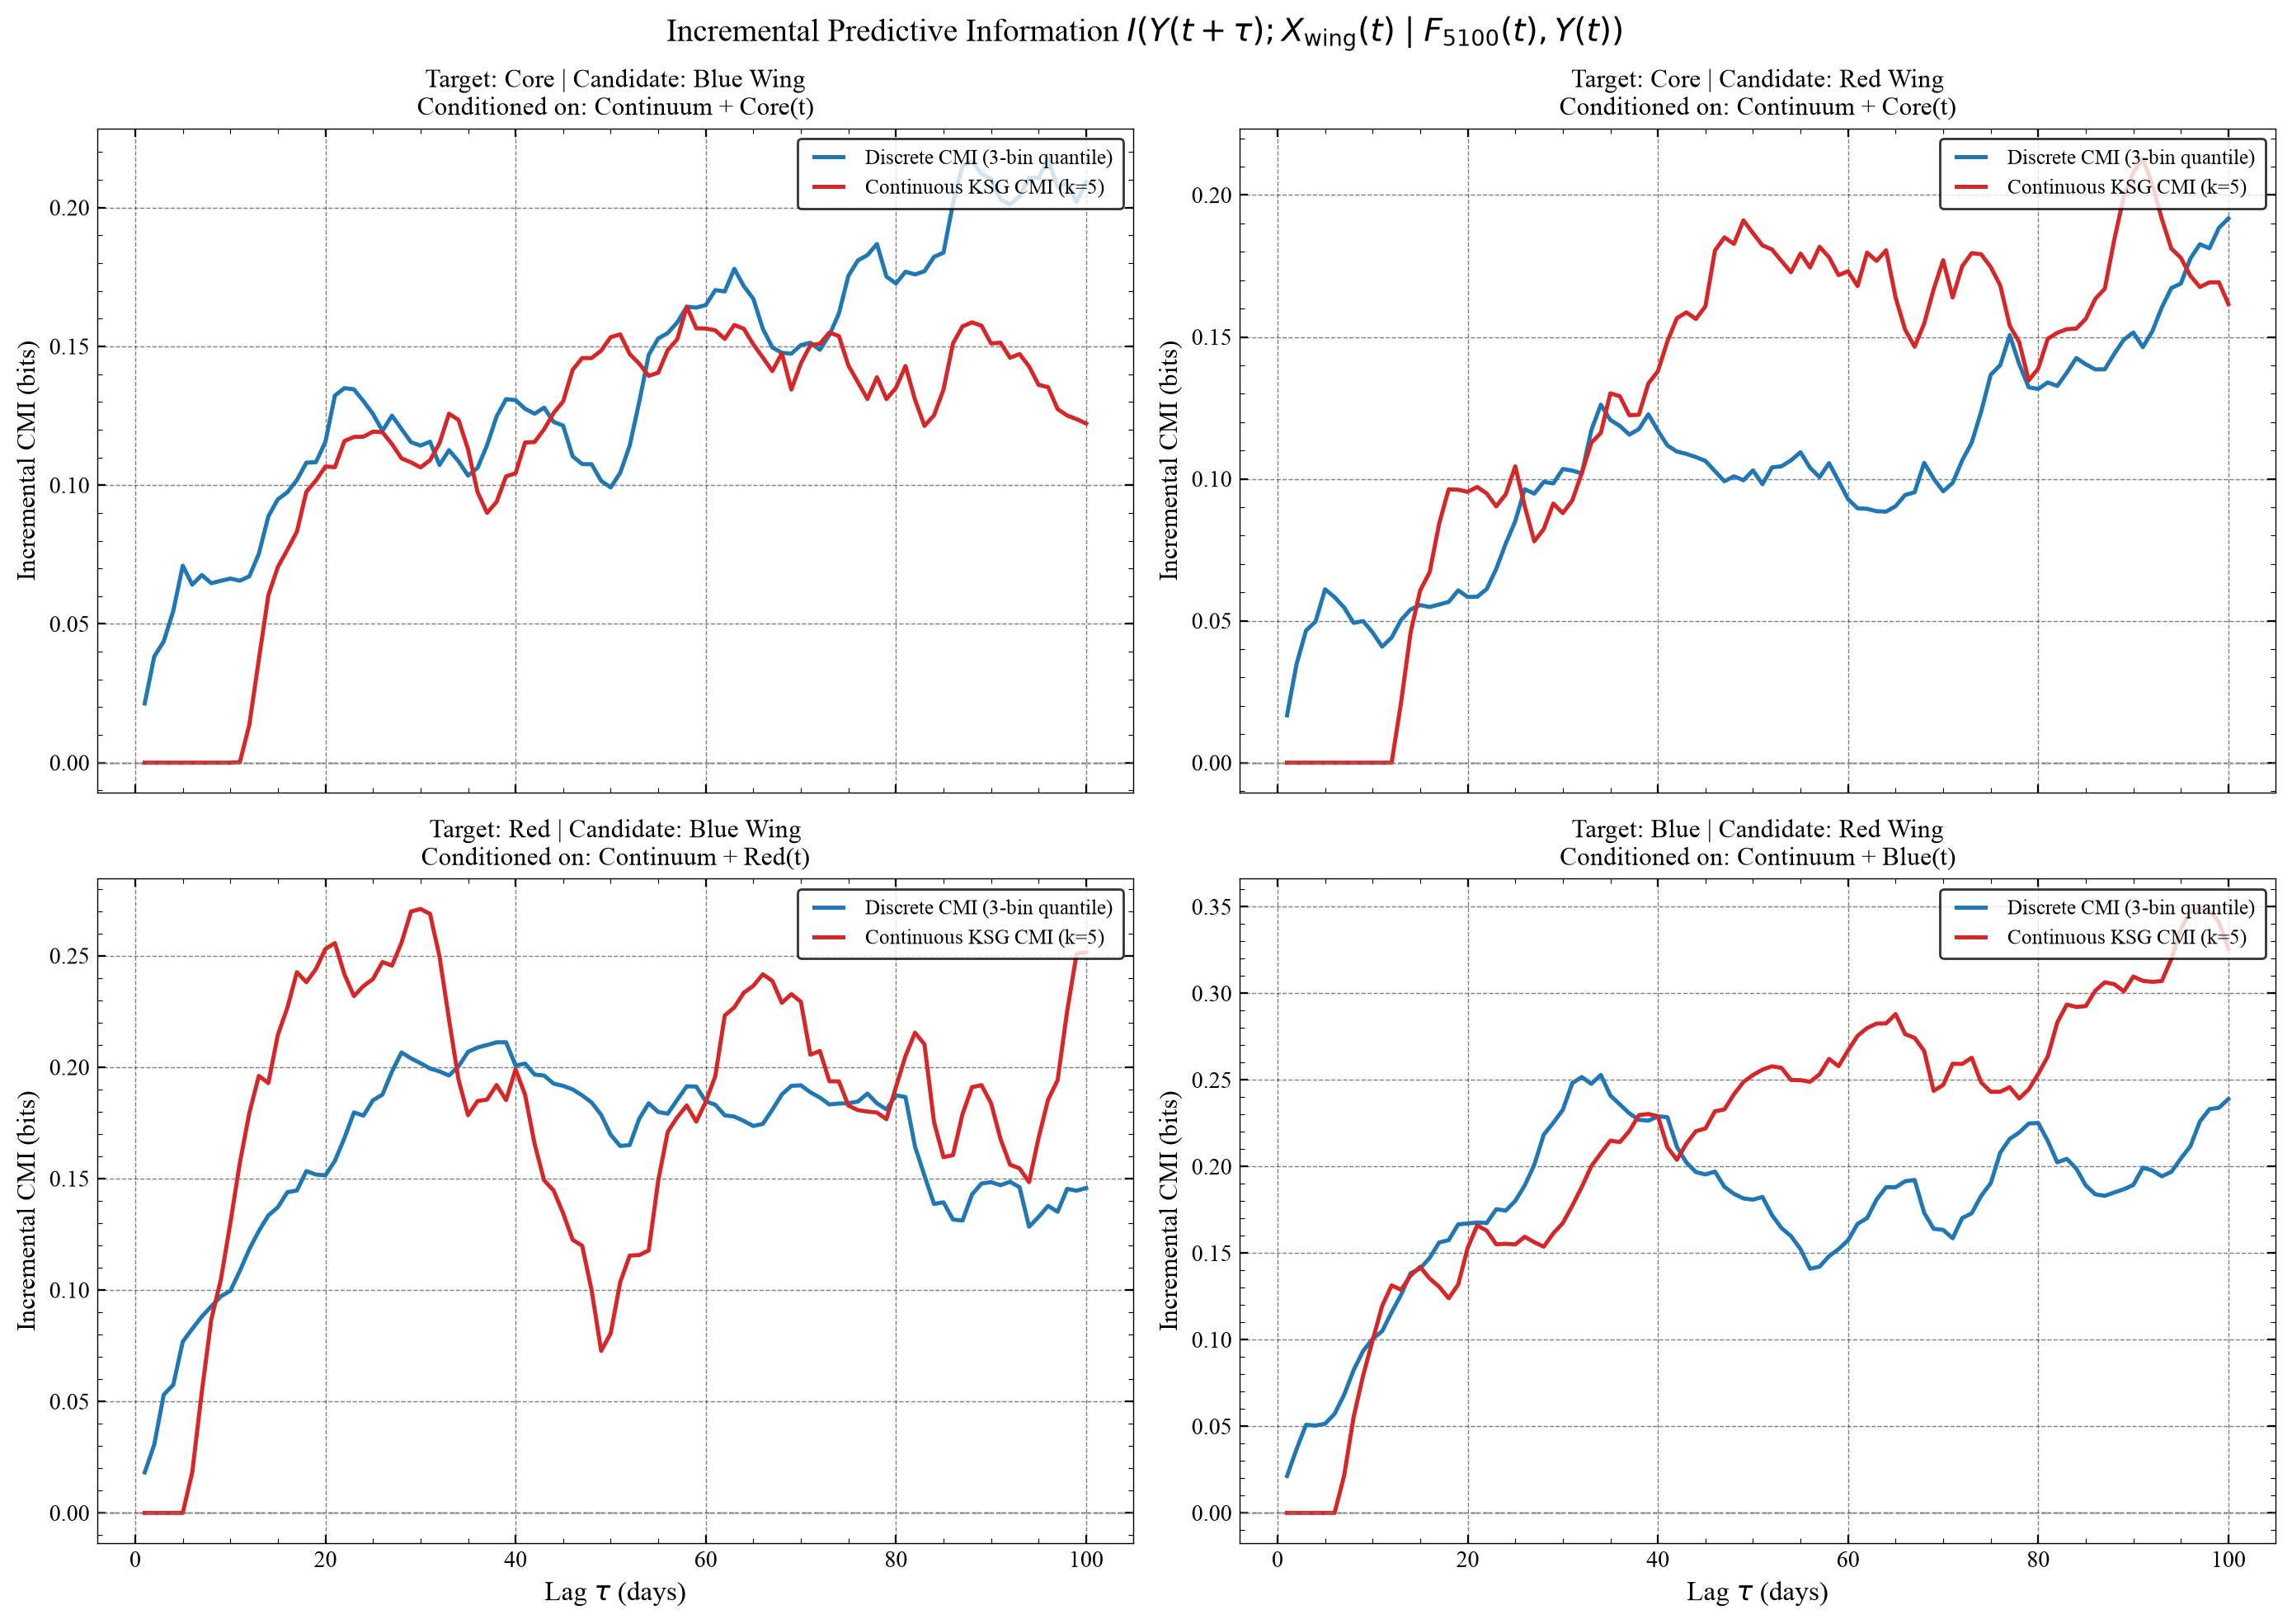
\includegraphics[width=0.98\textwidth]{figure13_incremental_information.png}
\caption{Conditional mutual information scans testing incremental velocity-component coupling. Solid curves show observed conditional mutual information $I(Y(t+\tau); X_{\mathrm{wing}}(t) \mid F_{5100}(t), Y(t))$ for discrete quantile histograms (blue) and continuous Kraskov KNN ($k=5$, green). Shaded bands and dashed lines represent the pointwise 95\% surrogate envelope and median from circular-shift realizations preserving the continuum and target history. In all four directional configurations, the observed curves lie well within their null envelopes ($p_{\mathrm{global}} \ge 0.61$--$1.00$).}
\label{fig:incremental_information}
\end{figure*}

We test four directional configurations:
\begin{enumerate}
    \item \textbf{Blue $\to$ Core:} Testing whether blue-wing gas predicts future core emission.
    \item \textbf{Red $\to$ Core:} Testing whether red-wing gas predicts future core emission.
    \item \textbf{Blue $\to$ Red (Outflow):} Testing whether the blueshifted wing leads and predicts the redshifted wing.
    \item \textbf{Red $\to$ Blue (Inflow):} Testing whether the redshifted wing leads and predicts the blueshifted wing.
\end{enumerate}
We evaluate conditional mutual information using both a discrete 3-bin quantile histogram estimator and a continuous Kraskov--St{\"o}gbauer--Grassberger (KSG, $k=5$) nearest-neighbor estimator. Statistical significance is determined using $N=30$ circular-shift surrogates in which $X_{\mathrm{wing}}$ is rolled while keeping the joint target-continuum pair $(Y(t+\tau), F_{5100}(t), Y(t))$ intact. Furthermore, we perform a leave-one-season-out predictive cross-validation, training a linear autoregressive predictor on four observing seasons and testing on the held-out season to record the change in out-of-sample explained variance $\Delta R^2$ when $X_{\mathrm{wing}}$ is added to the baseline.

Table~\ref{tab:incremental_information} and Figure~\ref{fig:incremental_information} demonstrate an unambiguous result: \textbf{once conditioned on the continuum driver and target autocorrelation, no velocity wing provides statistically significant incremental information about any other component}. Every directional scan yields a global $p$-value $p_{\mathrm{global}} \ge 0.61$--$1.00$ under both discrete and continuous estimators:
\begin{itemize}
    \item Blue $\to$ Core: discrete $p_{\mathrm{global}} = 0.903$, KNN $p_{\mathrm{global}} = 1.000$, $\Delta R^2 = +0.017$.
    \item Red $\to$ Core: discrete $p_{\mathrm{global}} = 1.000$, KNN $p_{\mathrm{global}} = 0.968$, $\Delta R^2 = -0.213$ (adding the Red wing degrades predictive accuracy).
    \item Outflow (Blue $\to$ Red): discrete $p_{\mathrm{global}} = 0.903$, KNN $p_{\mathrm{global}} = 0.677$.
    \item Inflow (Red $\to$ Blue): discrete $p_{\mathrm{global}} = 0.968$, KNN $p_{\mathrm{global}} = 0.613$, $\Delta R^2 = -0.053$.
\end{itemize}
Held-out out-of-sample predictive performance confirms this finding: adding a second velocity wing fails to improve predictive generalization, producing zero or negative $\Delta R^2$ across observing seasons. We conclude that the 1988--1993 NGC~5548 campaign data provide no evidence for direct kinematic coupling or directional gas transfer between velocity components; the observed multi-component variability is fully consistent with independent responses to a single ionizing continuum driver.

\subsection{Synthetic Benchmark Demonstrations}
\label{sec:synthetic_benchmarks}
To test the mathematical behavior of the histogram-based SURD pipeline under realistic observational conditions, we construct four synthetic benchmark models. The continuous driver signals are generated as damped random walk (DRW) processes on a 1-day grid, with pre-history included so that applying a delay does not wrap the end of a realization onto its beginning. The target signals are then constructed with known delays and couplings:
\begin{enumerate}
\item \textbf{Case 1: Single Driver.} The target responds to only one driver with a delay of 15.0 days.
\item \textbf{Case 2: Redundant Proxies.} The second driver is a noisy copy of the first. The target responds to the first driver with a 15.0-day delay.
\item \textbf{Case 3: Joint Nonlinear Drivers.} The target depends on the product of two independent drivers delayed by 15.0 days.
\item \textbf{Case 4: Two Independent Delayed Drivers.} The target is the additive response $0.5 S_1(t-10) + 0.5 S_2(t-20)$, where $S_1$ and $S_2$ are independent DRW processes.
\end{enumerate}

To match the observational footprint of the real campaign, the first predictor is sampled at the 557 continuum measurements and the second predictor and target are sampled at the 242 spectroscopic measurements (224 distinct dates in the adopted sample). Measurements sharing a date are averaged before interpolation. Gaussian noise is scaled by each channel's measured uncertainty relative to its observed flux standard deviation, and the sampled curves are interpolated back onto the 1-day grid. We run 100 independent Monte Carlo realizations, scan lags from 1 to 40~d, and record both lag recovery and whether the intended information atom is the largest atom at the true lag.

Figure~\ref{fig:synthetic_benchmarks} and Table~\ref{tab:synthetic_performance} separate simple positive controls from a harder two-delay stress test. Cases 1--3 recover the 15-day lag within $\pm5$~d in every realization, with mean biases smaller than 0.1~d. Their intended atoms are largest at the true lag in 100\%, 100\%, and 99\% of realizations, respectively. The additive two-delay case is substantially less reliable: the $U_1$ and $U_2$ diagnostics recover their associated lags within $\pm5$~d in only 67\% and 71\% of realizations, and are almost never the largest atom at the true lag. Thus, the estimator passes isolated-mechanism controls but does not reliably separate overlapping, autocorrelated responses.

The failure in Case 4 is visible in the median decomposition: broad synergy and redundancy exceed the individual unique terms even though the generating equation is additive. This is an important boundary on interpretation. A peak in a selected atom may locate a delay under a simple controlled mechanism, but the identity and amplitude of that atom cannot be mapped directly onto a physical coupling when multiple autocorrelated responses overlap. None of these prompt-lag tests supports interpreting the real 93--198~d maxima as displaced versions of 10--20~d reverberation delays.

\begin{table*}
\centering
\begin{tabular}{lcccccc}
\hline
\textbf{Case Model} & \textbf{True Lag} & \textbf{Diagnostic} & \textbf{Recovered Lag} & \textbf{Bias} & \textbf{Within $\pm5$~d} & \textbf{Atom Largest} \\
\hline
Case 1: Single Driver & 15 & $U_1$ & $15.0 \pm 0.8$ & $0.0$ & 1.00 & 1.00 \\
Case 2: Redundant Proxies & 15 & $R_{12}$ & $15.0 \pm 0.8$ & $+0.0$ & 1.00 & 1.00 \\
Case 3: Joint Nonlinear & 15 & $S_{12}$ & $15.0 \pm 1.2$ & $-0.0$ & 1.00 & 0.99 \\
Case 4: Driver 1 & 10 & $U_1$ & $8.4 \pm 8.4$ & $-1.6$ & 0.67 & 0.01 \\
Case 4: Driver 2 & 20 & $U_2$ & $24.9 \pm 5.8$ & $+4.9$ & 0.71 & 0.00 \\
\hline
\end{tabular}
\caption{Lag and information-atom recovery across 100 Monte Carlo realizations under the NGC~5548 sampling footprint. Recovered lags are means and sample standard deviations in days. ``Atom Largest'' is the fraction of realizations in which the designated atom exceeds the other three two-predictor atoms at the true lag.}
\label{tab:synthetic_performance}
\end{table*}

The positive controls establish that the implementation can recover simple isolated mechanisms under the observing window. The two-delay stress test shows that this success does not generalize to a more ambiguous multicomponent response, for which both lag recovery and atom identity degrade.

\begin{figure*}
\centering
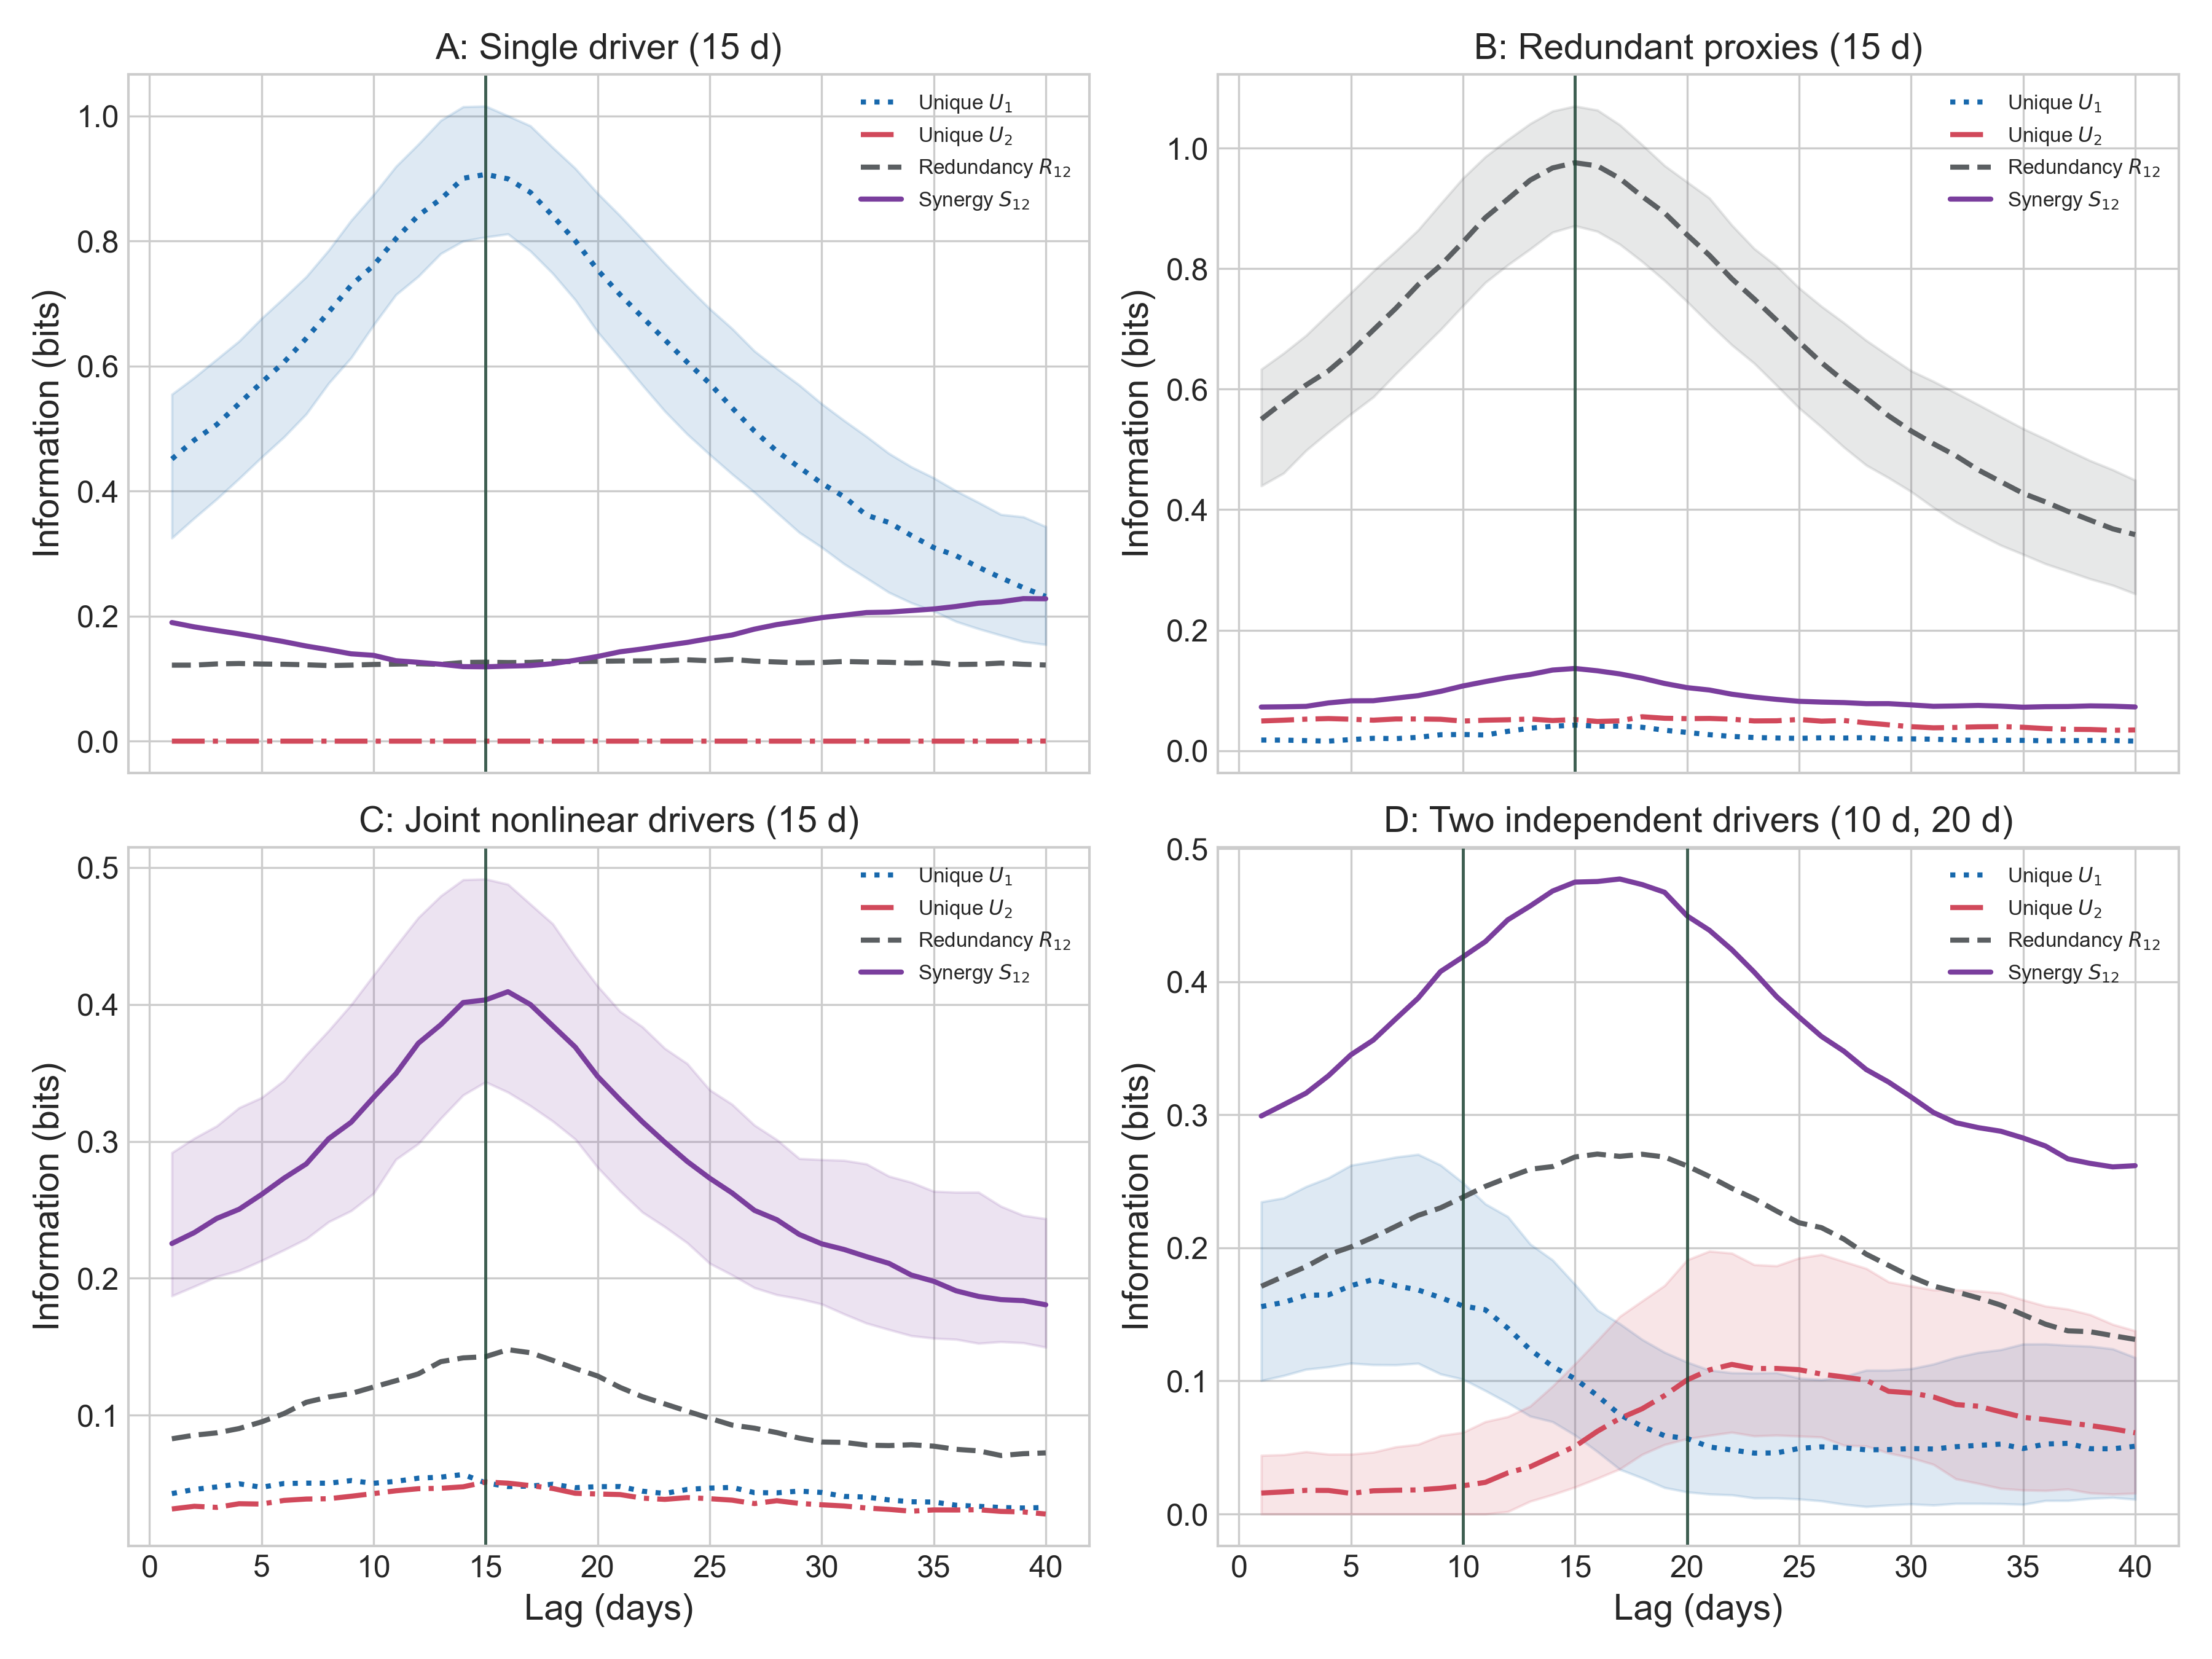
\includegraphics[width=0.95\textwidth]{figure5_synthetic_benchmarks.png}
\caption{Median SURD decompositions over 100 synthetic realizations sampled under the NGC~5548 observing footprint. Shading spans the 16th--84th percentiles for the designated diagnostic atom (two atoms in Case~4); vertical lines mark the true delays. Cases 1--3 recover their isolated generating mechanisms, whereas the additive two-delay stress test is dominated by broad synergy and redundancy.}
\label{fig:synthetic_benchmarks}
\end{figure*}

\iffalse
\subsection{Spurious Synergy Peaks from Seasonal Windowing (Negative Control)}
\label{sec:seasonal_aliasing_test}

To directly test whether the long-lag synergy peaks are physical or are artifacts of the observing window, we perform a synthetic negative control test. Ground-based AGN campaigns suffer from seasonal observing gaps (yearly periods of several months where the target cannot be observed), which are filled using linear interpolation.

We simulate $50$ Monte Carlo realizations of two independent Damped Random Walk (DRW) continuum drivers $S_1$ and $S_2$ ($\tau_{\mathrm{DRW}} = 50.0$~d and $30.0$~d). We generate a target line response $T_3$ driven strictly by a short-lag physical delay of $15.0$~days, with zero coupling at long lags:
\begin{equation}
T_3(t) = 0.5 S_1(t-15) + 0.5 S_2(t-15) + \eta(t),
\end{equation}
where $\eta(t)$ is independent Gaussian white noise. We then sample these signals at the exact observed dates ($\mathrm{JD} - 2400000$) of the real NGC~5548 campaign, add realistic observational flux errors, interpolate them back to a 1.0-day grid, and run the 2-predictor SURD scan up to $200$~days.

The resulting median synergy curve and null spreads are plotted in Figure~\ref{fig:seasonal_aliasing}. Crucially, even though there is zero physical coupling beyond $15$~days, the normalized synergy curve monotonically increases at large lags, reaching a median false synergy of $\sim 0.52$ at $75$~days, $\sim 0.55$ at $110$~days, and peaking at $\sim 0.59$ at $197$~days---values even higher than at the true coupling lag of $15$~days ($\sim 0.42$).

This spurious long-lag structure arises from two distinct mathematical and observational effects:
\begin{enumerate}
    \item \textbf{Interpolation-Induced Coherence (Red Noise Aliasing):} Linear interpolation across seasonal gaps smooths out high-frequency fluctuations, leaving only slow, low-frequency trends. This artificially inflates the apparent mutual information at large lags while suppressing joint entropy.
    \item \textbf{Normalized Synergy Inflation:} Normalized synergy is defined as $\widehat{S} = S / I(Y; X_1, X_2, X_3)$. Because the physical correlation between the continuum and the line vanishes at large lags, the joint mutual information $I(Y; X_1, X_2, X_3)$ in the denominator decreases to nearly zero. Dividing the remaining numerical estimation noise of $S$ by this tiny denominator results in massive inflation of the normalized synergy at long lags.
\end{enumerate}
This negative control test strongly shows that the unconditioned long-lag peaks observed in the real data (93--198 days) are fully consistent with seasonal windowing and normalized synergy inflation, and therefore do not require any physical long-lag BLR structure to explain them.

\begin{figure*}
\centering
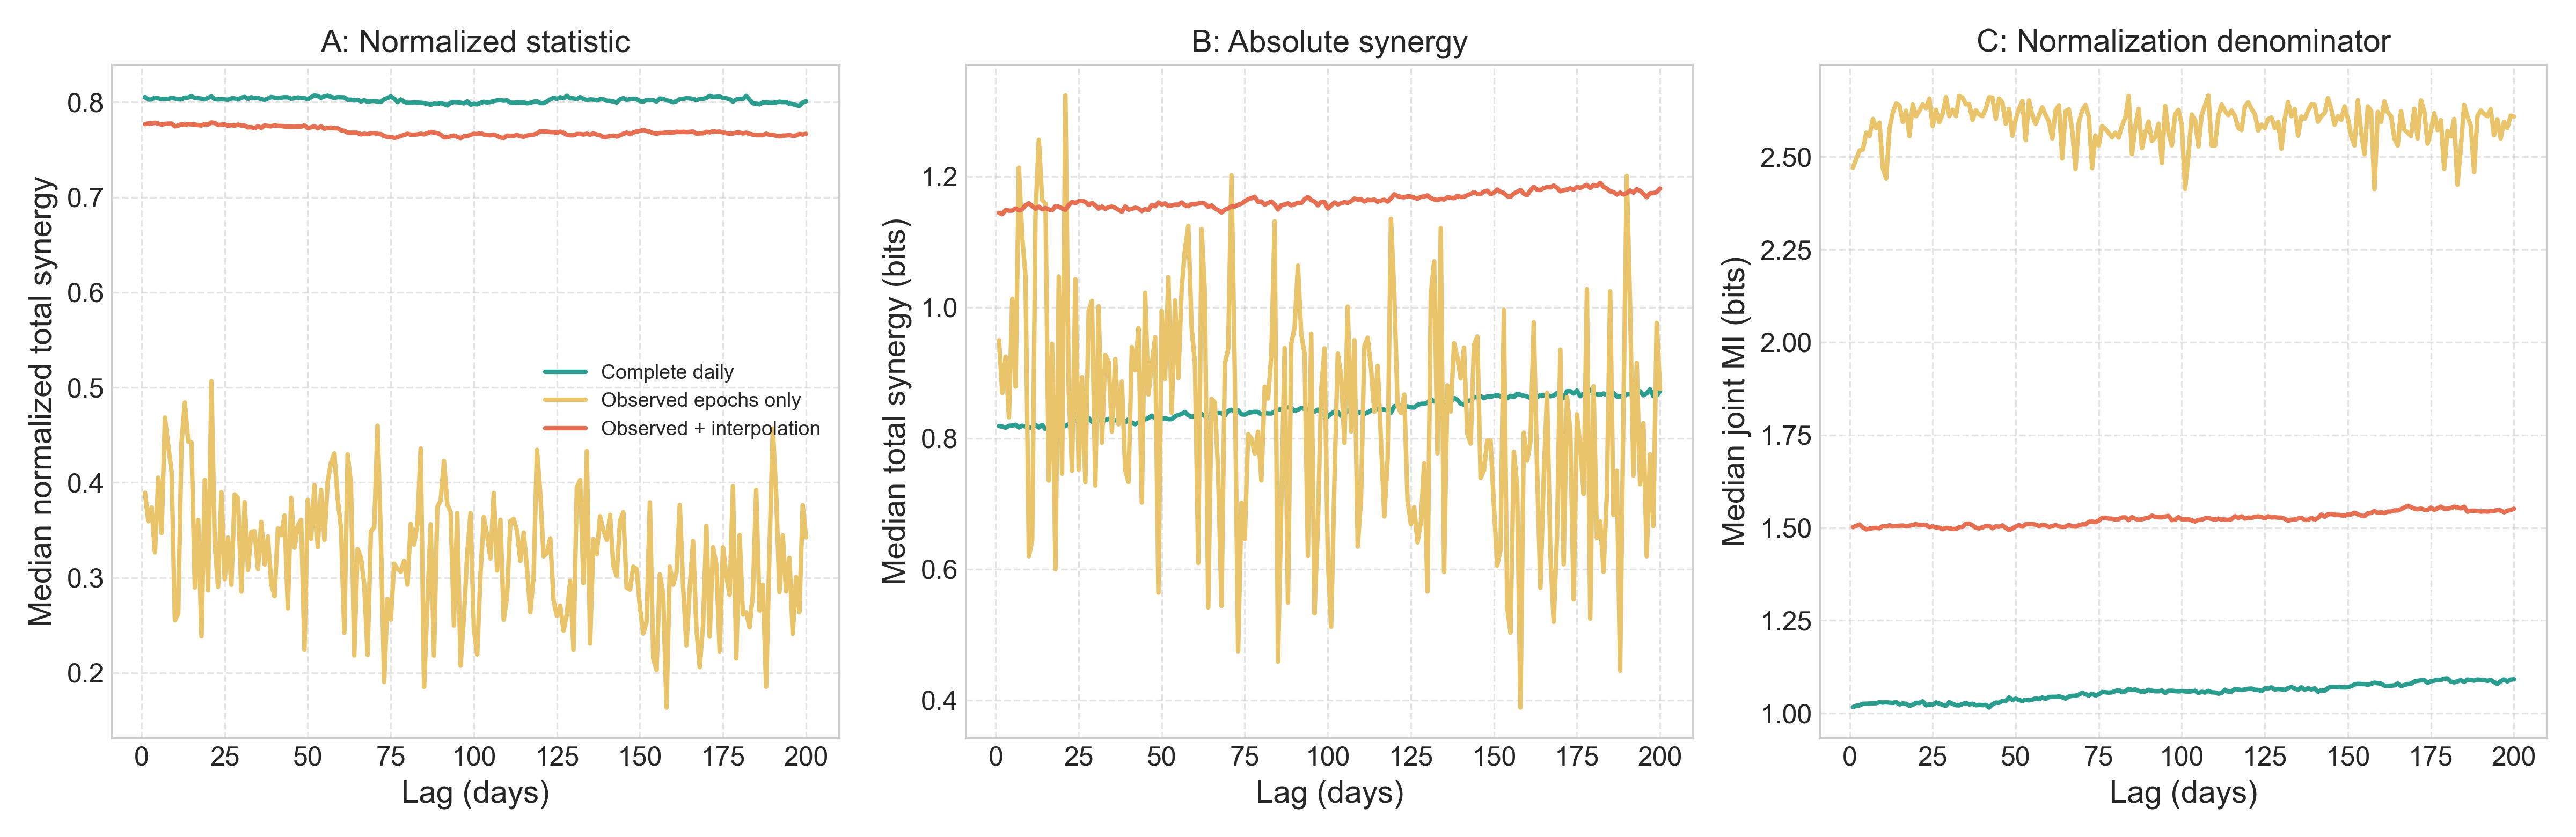
\includegraphics[width=0.95\textwidth]{figure7_seasonal_aliasing.png}
\caption{Spurious synergy curve generated by the seasonal observing window and linear interpolation in our negative control simulation (where the true coupling is strictly at 15 days). The false synergy rises monotonically at long lags, peaking at 197 days, exceeding the true 15-day peak. Vertical lines show the positions of the real H\(\beta\) peaks from NGC~5548.}
\label{fig:seasonal_aliasing}
\end{figure*}

\fi
\subsection{Matched Negative Control and Ablation}
\label{sec:seasonal_aliasing_test}

We next isolate an estimator-level null with no cross-channel coupling. For each of 200 realizations, we generate four independent Ornstein--Uhlenbeck red-noise series on the same 1744-d window and analyse the core analogue from the other three channels using the primary eight-bin, three-predictor, normalized 1--200~d scan. We compare (i) complete daily series, (ii) values retained only at exact observed continuum and spectroscopic epochs, and (iii) those observed values linearly interpolated back to the daily grid. At each stage we record normalized total synergy, absolute total synergy, joint mutual information, and the scan maximum.

Figure~\ref{fig:seasonal_aliasing} shows that large normalized values and scan-selected maxima occur despite complete independence. Their amplitude and location change under masking and interpolation, while absolute synergy and joint mutual information behave differently from their ratio. The exact-epoch calculation has only 11--40 usable matched tuples, depending on lag, and is therefore itself too sparse for a quantitative four-dimensional histogram estimate. This ablation does not identify one unique cause. It demonstrates the narrower claim required here: four-dimensional histogram sparsity, red-noise structure, the observing window, interpolation, and normalization are jointly sufficient to reproduce unstable false maxima. Interpolation alone is not assigned a causal effect.

\begin{figure*}
\centering
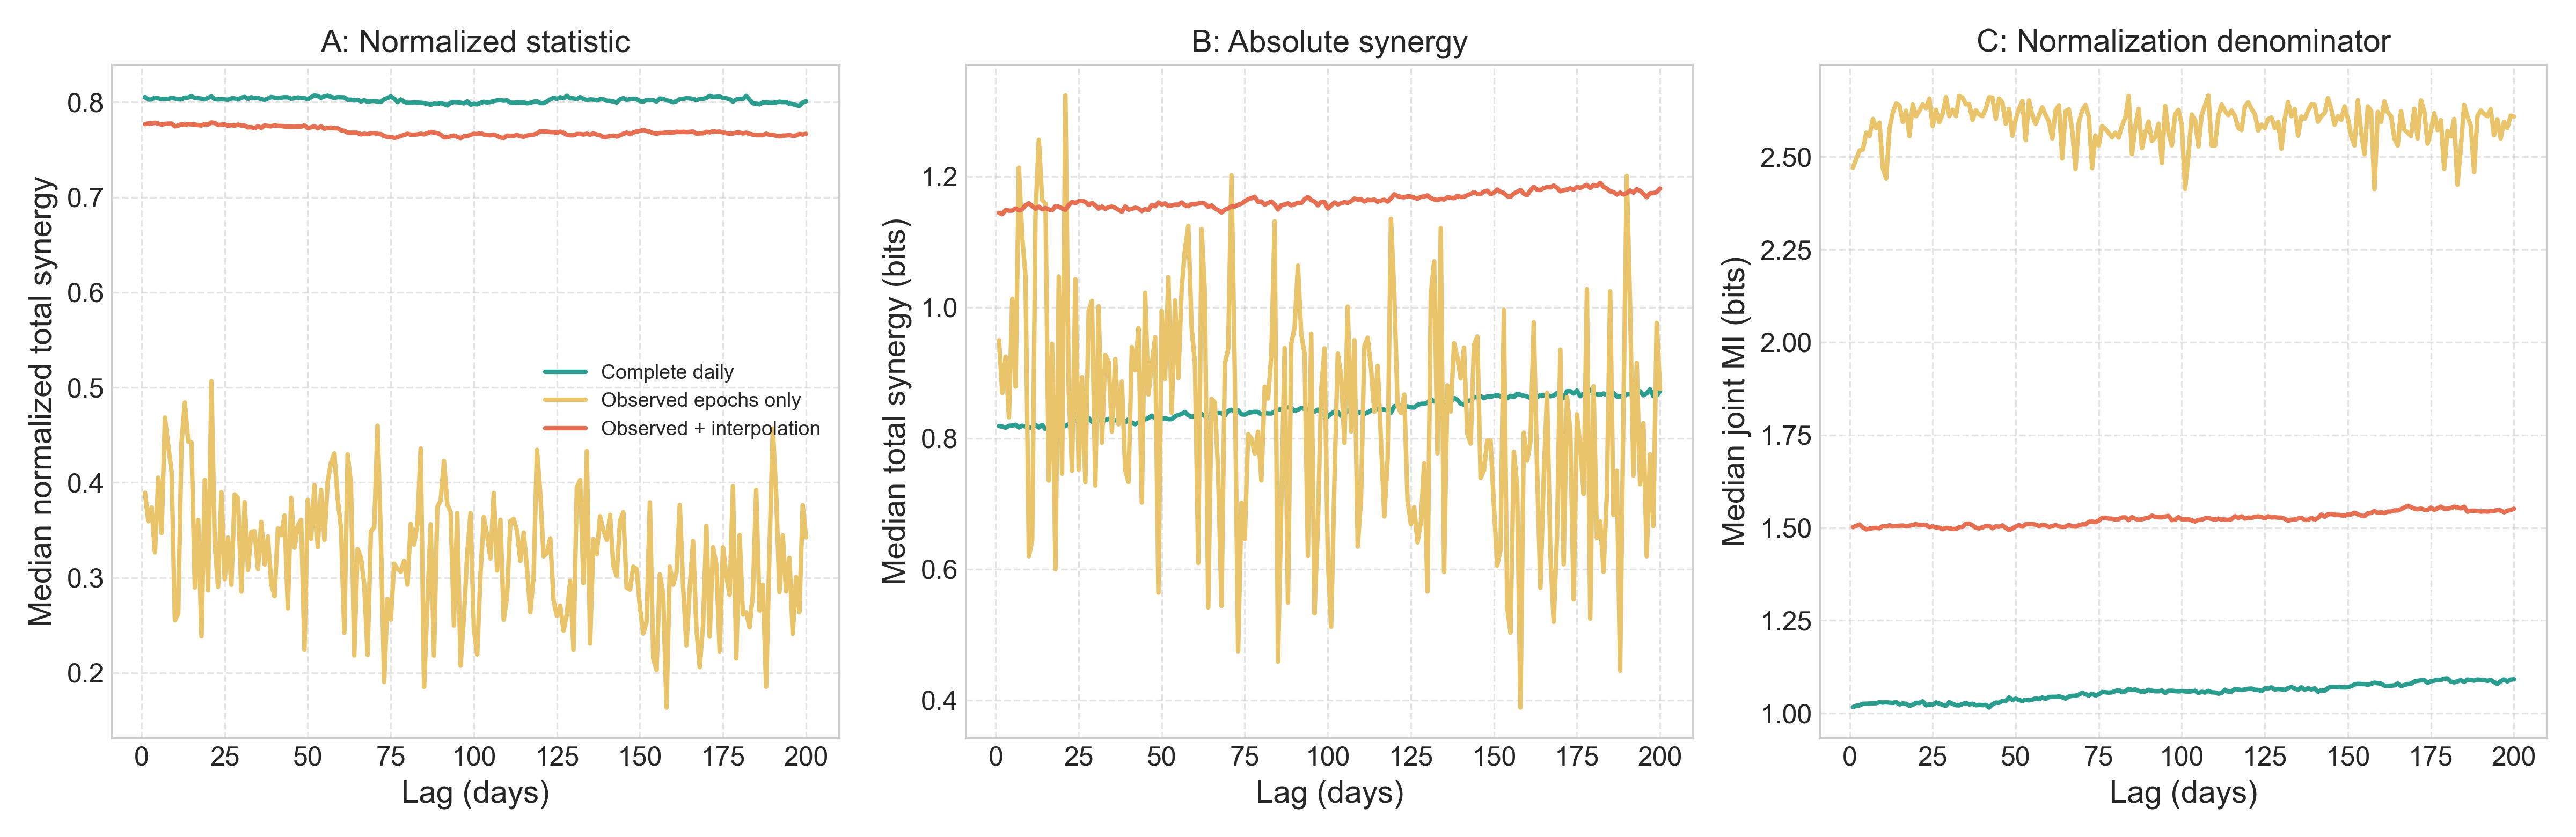
\includegraphics[width=0.98\textwidth]{figure7_seasonal_aliasing.png}
\caption{Matched three-predictor negative-control ablation over 200 independent red-noise realizations. Curves show medians for complete daily data, exact observed epochs, and observed epochs followed by daily interpolation. The panels separate normalized total synergy, absolute total synergy, and its joint-MI normalization denominator. The observed-only estimate is shown diagnostically but is severely undersampled.}
\label{fig:seasonal_aliasing}
\end{figure*}

\subsection{Target-History Conditioning and Autocorrelation}
\label{sec:target_history_conditioning}

A key challenge in information-theoretic analyses of astronomical time series is distinguishing true cross-component information flow from the target signal's own autocorrelation (red-noise memory). If a target component (such as Core H\(\beta\)) is strongly autocorrelated on short timescales, the apparent synergy between predictors could simply reflect the target's memory rather than direct physical coupling from the driving continuum.

To address this, we perform a target-history conditioned SURD scan. We decompose the conditional mutual information:
\begin{equation}
I(Y(t+\tau); X_1(t), X_2(t) \mid X_3(t))
\end{equation}
where $Y = \mathrm{Core}(t+\tau)$ is the future state of the target Core, $X_1 = \mathrm{Continuum}(t)$ and $X_2 = \mathrm{Blue\ Wing}(t)$ are the predictors, and $X_3 = \mathrm{Core}(t)$ is the target's own past state. This conditional Partial Information Decomposition (conditional PID) is calculated by binning the joint 4D space, extracting the 3D slices for each bin of $X_3$, running the standard SURD decomposition on each slice, and taking the probability-weighted sum of the results.

The results of this comparison are shown in Figure~\ref{fig:history_conditioning}. Because the conditional surrogate suite was generated only over 1--120~d, we restrict the comparison to that same window. Within this tested range, the unconditioned synergy curve peaks at \textbf{9 days} ($0.316$~bits), reflecting strong short-term autocorrelation of the light curve, while the history-conditioned curve reaches its local maximum at \textbf{73 days} ($0.309$~bits).

However, surrogate significance tests and bin occupancy analysis show that this conditional peak is not statistically significant:
\begin{enumerate}
    \item \textbf{Conditional Surrogate Significance:} We run $100$ circular-shift surrogates for the conditional scan to estimate the global null distribution of the max-statistic. The real peak conditional synergy ($0.3092$ bits) is well below the median of the global null max-statistic ($0.4043$ bits), yielding a global $p$-value of \textbf{0.9802}. This indicates that the conditioned peak is statistically indistinguishable from random noise.
    \item \textbf{High-Dimensional Sample Sparsity:} The conditional decomposition requires binning a 4D joint space. The daily strict-overlap grid has $N=1744$, but a lag $\tau$ uses $N_{\rm eff}(\tau)=1744-\tau$ tuples. Thus the 73-d conditional maximum has $N_{\rm eff}=1671$. For $n_{\mathrm{bins}}=6$, the $6^4=1296$ cells are 89.20\% empty (1156 cells), with only 11.9 samples per occupied cell on average. This severe sparsity biases the histogram information estimates.
\end{enumerate}
We then repeat the complete 1--120~d conditional scan with 3--8 bins using both equal-width and quantile discretization. For every setting, we generate 49 additional circular-shift realizations and compare the observed maximum with the distribution of surrogate maxima. Table~\ref{tab:conditional_binning} and Figure~\ref{fig:conditional_binning} show that the inferred peak is not stable: equal-width peaks span 37--97~d and quantile-bin peaks span 71--102~d. The estimated peak amplitude also grows strongly with bin count as the joint histogram becomes sparser. Despite these changes, every auxiliary global test is non-significant, with empirical $p_{\mathrm{global}}$ values from 0.64 to 1.00. The 49-surrogate auxiliary tests have a $p$-value resolution of 0.02 and are intended as sensitivity checks; the primary six-bin significance result remains the 100-surrogate value $p_{\mathrm{global}}=0.9802$ quoted above.

Consequently, within the tested 1--120~d window, the conditional peak is better interpreted as a discretization- and finite-sample-dependent feature than as a resolved physical coupling. The robust result is the absence of global significance, not the location of any individual maximum.

\begin{table*}
\centering
\begin{tabular}{lccccc}
\hline
\textbf{Binning} & \textbf{Bins} & \textbf{Peak Lag (d)} & \textbf{Peak $S_{12}$ (bits)} & \textbf{Empty Cells} & $\boldsymbol{p}_{\mathbf{global}}$ \\
\hline
Equal width & 3 & 62 & 0.080 & 58.0\% & 0.96 \\
Equal width & 4 & 37 & 0.146 & 77.7\% & 0.98 \\
Equal width & 5 & 74 & 0.223 & 83.8\% & 0.94 \\
Equal width & 6 & 73 & 0.309 & 89.2\% & 0.96 \\
Equal width & 7 & 60 & 0.408 & 92.3\% & 0.92 \\
Equal width & 8 & 97 & 0.467 & 94.5\% & 0.94 \\
Quantile & 3 & 71 & 0.146 & 29.6\% & 0.96 \\
Quantile & 4 & 85 & 0.320 & 55.1\% & 1.00 \\
Quantile & 5 & 92 & 0.428 & 70.4\% & 0.98 \\
Quantile & 6 & 92 & 0.572 & 80.9\% & 0.80 \\
Quantile & 7 & 97 & 0.679 & 87.1\% & 0.72 \\
Quantile & 8 & 102 & 0.725 & 91.0\% & 0.64 \\
\hline
\end{tabular}
\caption{Sensitivity of the core-target history-conditioned scan to histogram construction. Empty-cell fractions are evaluated at each setting's observed maximum. Empirical global $p$-values use 49 auxiliary circular-shift surrogate maxima per setting. None is significant at $\alpha=0.05$.}
\label{tab:conditional_binning}
\end{table*}

\begin{figure*}
\centering
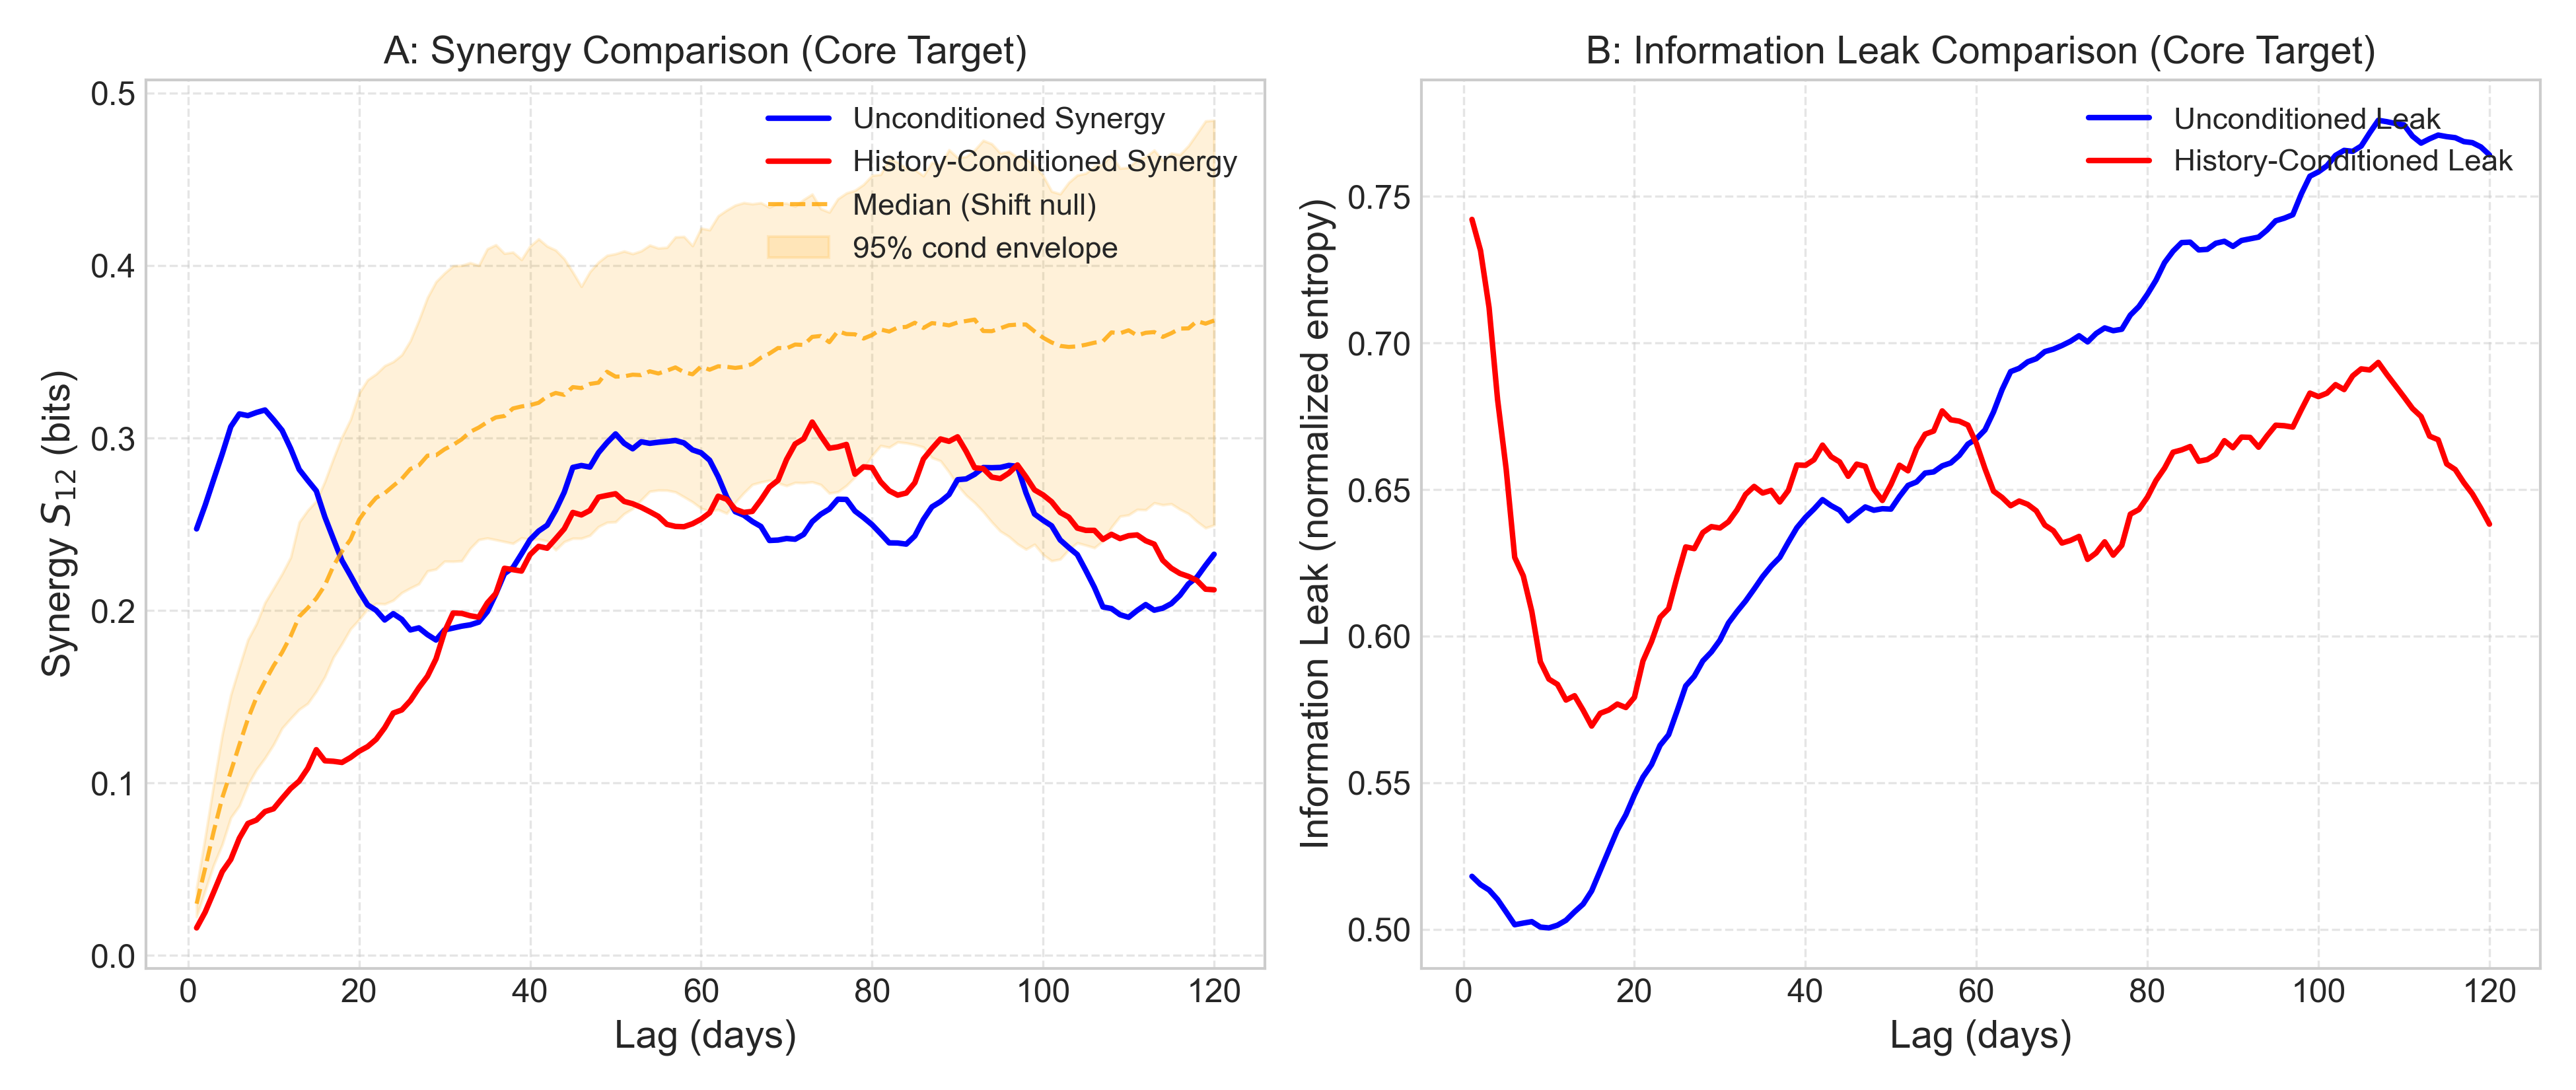
\includegraphics[width=0.95\textwidth]{figure8_history_conditioning.png}
\caption{Comparison of the unconditioned (blue) and target-history conditioned (red) SURD synergy (left) and information leak (right) curves for the Core H\(\beta\) target over the 1--120~d window for which conditional surrogates were computed. The orange shaded band and dashed line represent the pointwise 95\% circular-shift surrogate envelope and median at each lag for the conditioned scan. The global max-statistic test compares the observed peak to the distribution of per-realization surrogate maxima (whose median is $0.4043$~bits, with the 95th percentile higher) and is not represented by a single pointwise threshold curve. Within this tested window, conditioning on the target's own past shifts the local synergy peak to 73 days, but the peak is statistically insignificant ($p_{\mathrm{global}} = 0.9802$) under this null and does not establish physical coupling.}
\label{fig:history_conditioning}
\end{figure*}

\begin{figure*}
\centering
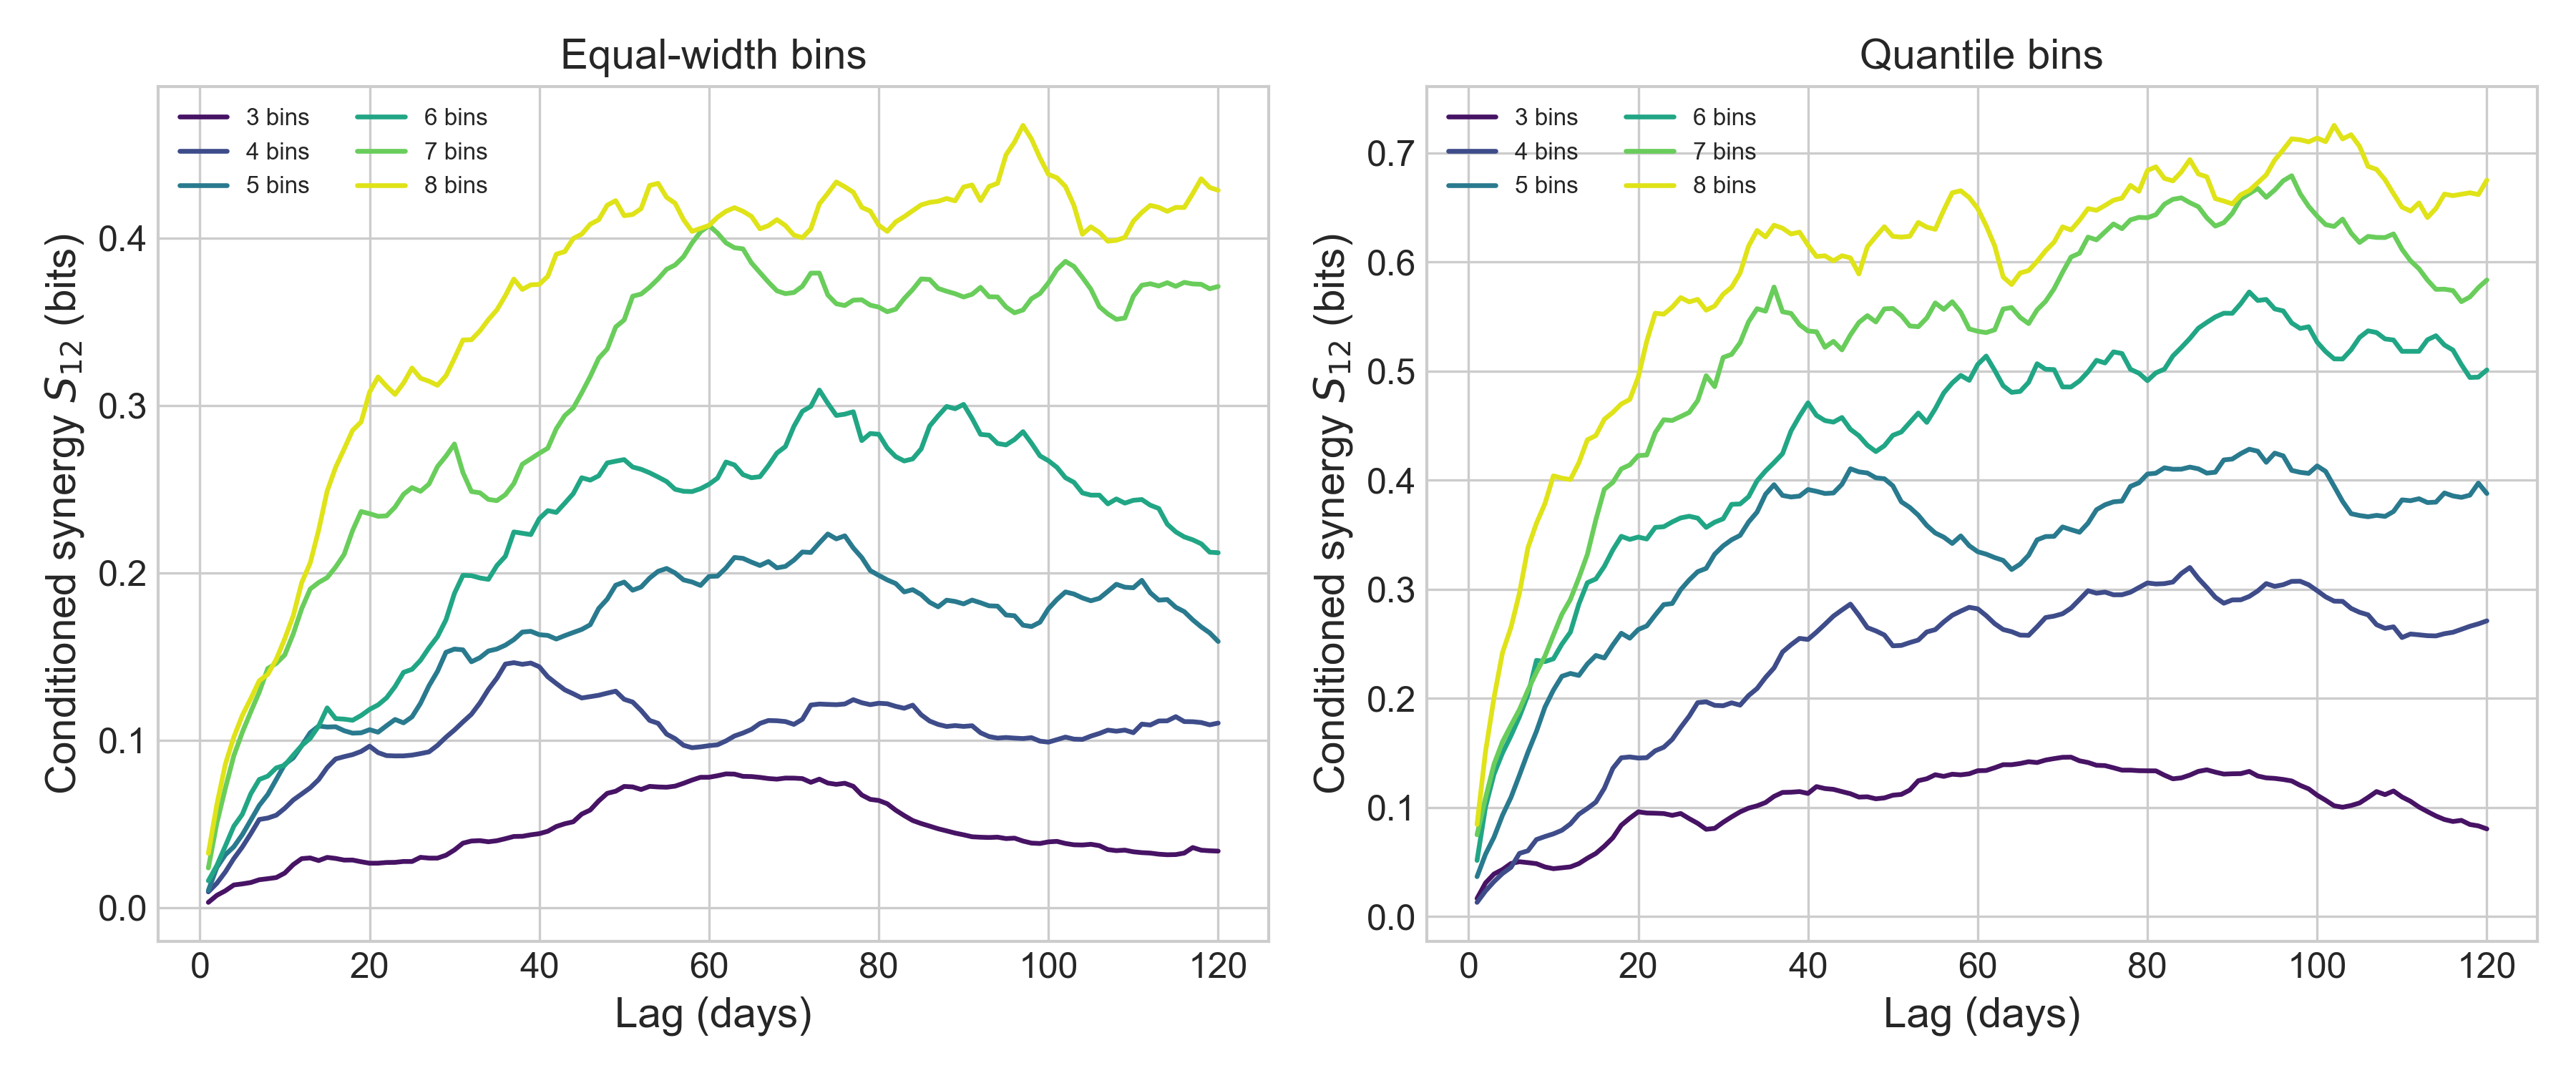
\includegraphics[width=0.95\textwidth]{figure9_conditional_binning_sensitivity.png}
\caption{History-conditioned core-target synergy over 1--120~d for 3--8 equal-width bins (left) and quantile bins (right). Both peak amplitude and peak location vary with discretization; increasing the number of bins systematically inflates the estimated synergy as occupancy declines.}
\label{fig:conditional_binning}
\end{figure*}

\subsection{Dimensionality Limits and Estimator Scaling}
\label{sec:dimensionality_limits}

The severe sparsity encountered in the target-history conditioned scan (Section~\ref{sec:target_history_conditioning}) highlights a fundamental limitation of histogram-based information-theoretic estimators: the exponential scaling of the joint probability cell count with the number of variables (the "curse of dimensionality"). 

To quantify this effect, we record occupancy at each primary maximum. The $8^4=4096$-cell histograms use $N_{\rm eff}=1629$, 1546, 1616, and 1651 tuples at the continuum (115~d), red (198~d), core (128~d), and blue (93~d) maxima. Their empty-cell fractions are 93.82\%, 93.65\%, 93.19\%, and 93.04\%, respectively. Thus the effective sample count and occupancy are explicitly lag-dependent, and the four-dimensional histogram estimates remain exploratory.

Adding target history as a fourth predictor with eight bins would require $8^5=32,768$ cells for at most 1743 lagged tuples, or fewer than 0.054 samples per cell even before accounting for nonuniform occupancy. We therefore do not attempt that histogram decomposition.

Consequently, the 3-predictor round-robin scans can at most identify exploratory information profiles, while full 4-predictor joint reconstructions are out of reach using standard histograms. To test whether the principal lag and significance conclusions depend on histogram sparsity, we perform the continuous-estimator cross-check below.

\subsection{Continuous-Estimator Cross-Check}
\label{sec:knn_crosscheck}

We estimate total mutual information between each future target and the other three present channels using the Kraskov--St{\"o}gbauer--Grassberger (KSG) $k$-nearest-neighbour estimator \citep{Kraskov2004}. For samples $i=1,\ldots,N$, the estimator uses the distance to each sample's $k$th neighbour in the joint space and counts neighbours $n_x(i)$ and $n_y(i)$ in the corresponding marginal spaces,
\begin{equation}
\widehat I_{\mathrm{KSG}} = \psi(k)+\psi(N)-\left\langle\psi[n_x(i)+1]+\psi[n_y(i)+1]\right\rangle_i,
\end{equation}
where $\psi$ is the digamma function. We use the Chebyshev metric, add deterministic jitter of $10^{-10}$ times the marginal scale to break exact interpolation ties, and repeat the calculation for $k=3$, 5, and 10. We also estimate $I(Y;X_1,X_2\mid Y_{\mathrm{past}})$ with the nearest-neighbour conditional mutual-information estimator of \citet{FrenzelPompe2007}. Significance is evaluated with 999 independent circular-shift realizations using the same global maximum-statistic procedure as the histogram analysis.

Table~\ref{tab:knn_crosscheck} reports the central $k=5$ results; $k=3$ and 10 give the same qualitative conclusion. Total KNN mutual information identifies globally significant prompt maxima at 1~d for the three line targets ($p_{\mathrm{global}}=0.001$ for $k=5$). In contrast, none of the maxima restricted to 61--200~d is significant: across all three $k$ choices, $p_{\mathrm{global}}=0.167$--0.271 for the Blue Wing, 0.418--0.466 for the Core, 0.592--0.888 for the Red Wing, and 0.861--0.911 for the Continuum. Values evaluated directly at the histogram-SURD maxima are also non-significant ($p=0.194$--0.907). Finally, the history-conditioned scan is globally non-significant for every neighbourhood size ($p_{\mathrm{global}}=0.977$--0.985), and its value at 73~d is pointwise non-significant ($p=0.915$ for $k=5$).

This cross-check does not reproduce the SURD atom decomposition and is not presented as an alternative unique--redundant--synergistic partition. It establishes a narrower but important result: a continuous estimator independently recovers strong prompt multivariate dependence while providing no evidence that the reported long-lag SURD maxima represent significant predictive dependence.

\begin{table*}
\centering
\begin{tabular}{lcccccc}
\hline
\textbf{Target} & \textbf{Peak Lag} & $\boldsymbol{p}_{\mathbf{1--200}}$ & \textbf{Long-Lag Peak} & $\boldsymbol{p}_{\mathbf{61--200}}$ & \textbf{SURD Peak} & $\boldsymbol{p}_{\mathbf{at~SURD}}$ \\
\hline
Continuum & 94 & 0.942 & 94 & 0.861 & 115 & 0.862 \\
Blue Wing & 1 & 0.001 & 168 & 0.167 & 93 & 0.216 \\
Core & 1 & 0.001 & 61 & 0.418 & 128 & 0.493 \\
Red Wing & 1 & 0.001 & 164 & 0.787 & 198 & 0.681 \\
Core conditional & 77 & 0.977 & -- & -- & 73 & 0.915 \\
\hline
\end{tabular}
\caption{Continuous KNN estimator cross-check for $k=5$ using 999 circular-shift surrogates. Peak lags are in days. The first global $p$-value covers the full scan (1--200~d for total MI and 1--120~d for conditional MI); the long-lag test is restricted to 61--200~d. The final column is pointwise at the corresponding histogram-SURD maximum and is not a global test.}
\label{tab:knn_crosscheck}
\end{table*}

\begin{figure*}
\centering
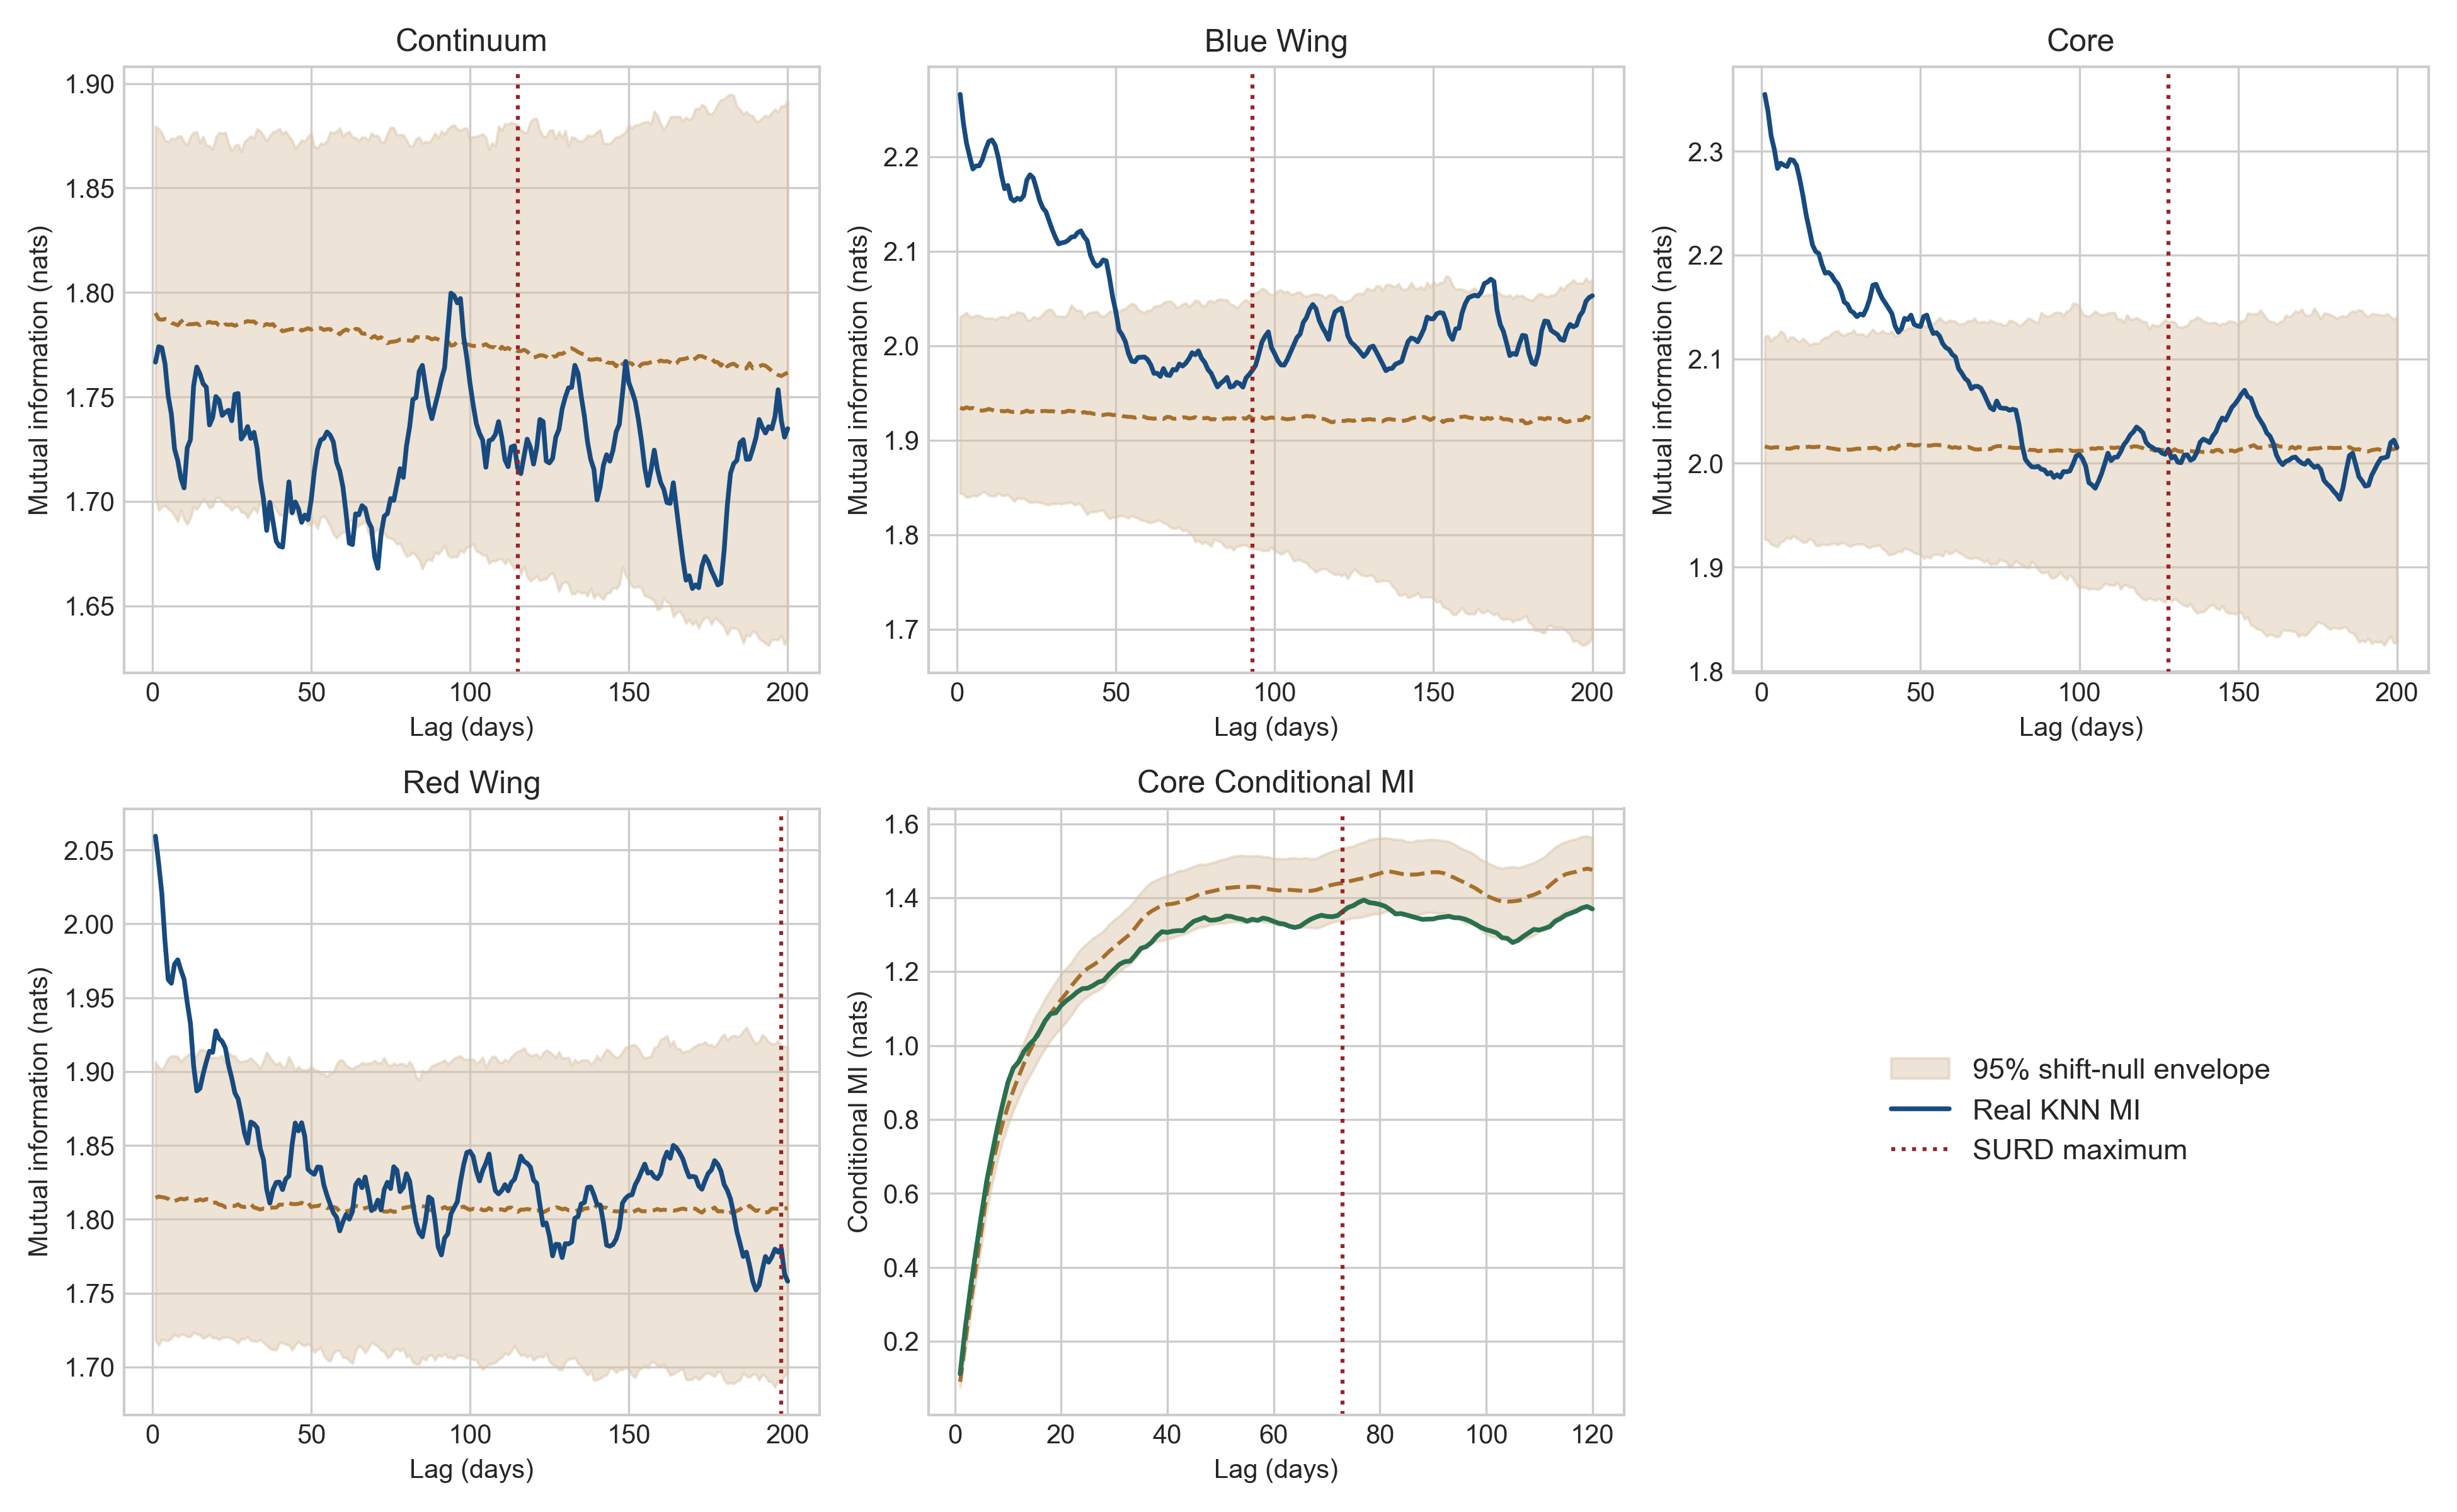
\includegraphics[width=0.98\textwidth]{figure10_knn_crosscheck.png}
\caption{KNN mutual-information cross-check for $k=5$. Blue or green curves show the real total or conditional mutual information, tan bands show pointwise 95\% circular-shift envelopes, and dotted red lines mark the corresponding histogram-SURD maxima. Prompt dependence is visible for the three line targets, whereas the long-lag SURD maxima and the conditioned 73-day maximum lie within their null distributions.}
\label{fig:knn_crosscheck}
\end{figure*}

\subsection{Independent-Object Check with Mrk 817}
\label{sec:mrk817_replication}

We next test whether the estimator-sensitivity seen in NGC~5548 is specific to that object. We use the public AGN STORM~2 HST/COS light curves of Mrk~817: 165 synchronized visits spanning 456.6~d, with a median cadence of 2.0~d, for the 1180-\AA\ continuum and Ly$\alpha$, N\,V, Si\,IV, C\,IV, and He\,II emission lines \citep{Homayouni2023,STORM2HLSP2023}. Published rest-frame continuum--line delays range from 8.2 to 15.5~d \citep{Homayouni2023}.

Because this campaign contains gaps of 36 and 51~d, we do not interpolate it onto a daily grid. At each integer observed-frame lag from 0 to 40~d, continuum and line measurements are instead paired one-to-one when their actual separation is within 1.1~d of the requested lag. We estimate bivariate KSG mutual information for $k=3$, 5, and 10, and compare each curve with 999 circular shifts of the corresponding line fluxes. We report a line-wise maximum-statistic $p$-value, a stricter family-wise value based on the largest statistic across all five lines and lags, and a separate five-line family-wise test at the externally specified published delays. Pairing tolerances of 0.75 and 1.5~d provide a sensitivity check.

Table~\ref{tab:mrk817_replication} gives the central $k=5$ results. At the published delays, Ly$\alpha$ and C\,IV remain significant after the five-line correction ($p=0.027$ and 0.001), whereas N\,V, Si\,IV, and He\,II do not ($p=0.053$, 0.065, and 0.993). The unrestricted scan is less stable: only N\,V narrowly survives the five-line, 0--40~d correction for $k=5$ ($p=0.048$), but its maximizing lag is 5~d rather than the published 15.5~d and moves between 5 and 15~d as the pairing tolerance and $k$ change. The other four $k=5$ maxima have family-wise $p=0.171$--1.000. Thus the independent object contains real information near some externally measured delays, but maximizing an unrestricted information curve does not yield a generally stable lag estimator. This supports the methodological conclusion from NGC~5548 without extending the SURD atom decomposition to a sample too small for a reliable multidimensional histogram.

\begin{table*}
\centering
\begin{tabular}{lccccc}
\hline
\textbf{Line} & \textbf{MI peak} & $\boldsymbol{p}_{\mathbf{line}}$ & $\boldsymbol{p}_{\mathbf{5\,lines}}$ & \textbf{Published lag} & $\boldsymbol{p}_{\mathbf{published,5\,lines}}$ \\
\hline
Ly$\alpha$ & 14 & 0.137 & 0.424 & 10.4 & 0.027 \\
N\,V       & 5  & 0.001 & 0.048 & 15.5 & 0.053 \\
Si\,IV     & 9  & 0.080 & 0.876 & 8.2  & 0.065 \\
C\,IV      & 19 & 0.085 & 0.171 & 11.8 & 0.001 \\
He\,II     & 10 & 0.126 & 1.000 & 9.0  & 0.993 \\
\hline
\end{tabular}
\caption{Independent Mrk~817 KNN check for $k=5$ using 999 circular-shift surrogates. MI-peak lags are observed-frame days; published lags are rest-frame days from \citet{Homayouni2023}. The two maximum-statistic columns correct over 0--40~d for one line and all five lines, respectively. The final column corrects across the five externally specified literature lags.}
\label{tab:mrk817_replication}
\end{table*}

\begin{figure*}
\centering
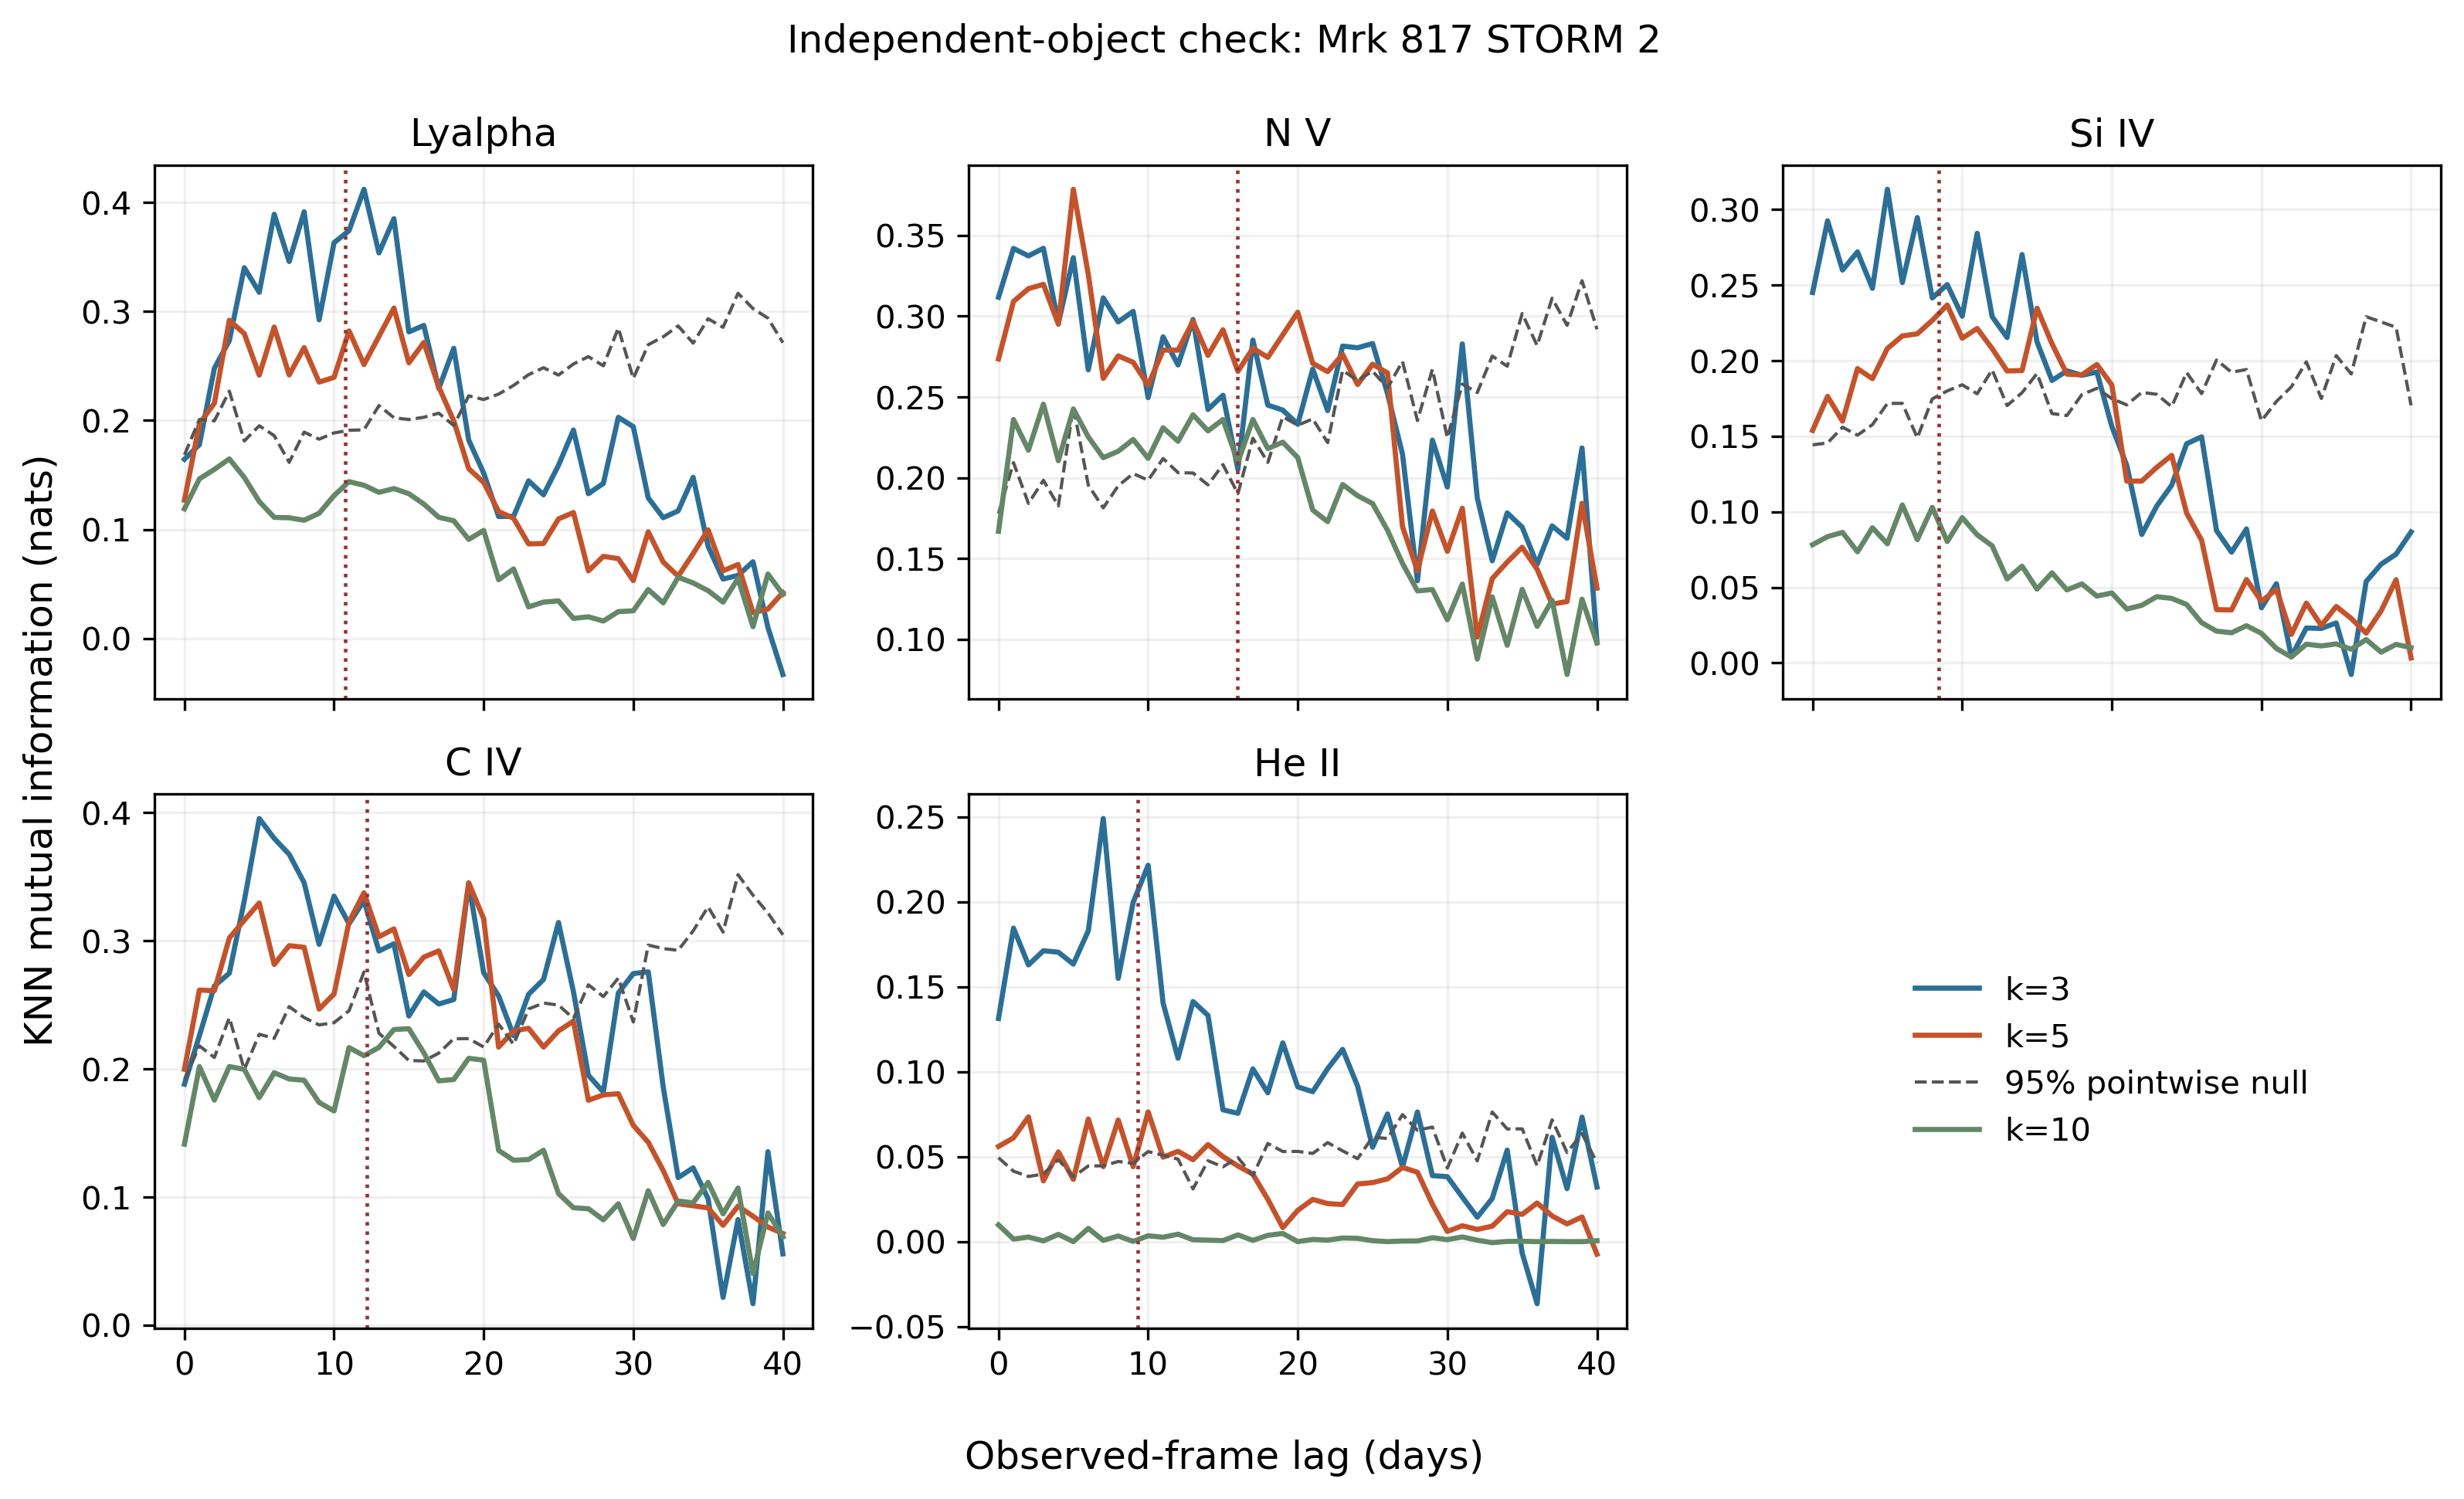
\includegraphics[width=0.98\textwidth]{figure11_mrk817_replication.png}
\caption{Native-cadence KNN mutual-information scans for Mrk~817. Coloured curves show $k=3$, 5, and 10; grey dashed curves are the pointwise 95\% circular-shift envelopes for $k=5$; dotted red lines mark the observed-frame equivalents of the published delays. Pointwise excursions are not equivalent to the scan-wide tests in Table~\ref{tab:mrk817_replication}.}
\label{fig:mrk817_replication}
\end{figure*}

\section{Interpretation and Methodological Implications}
\label{sec:discussion}

The results in Section~\ref{sec:results} reveal a discrepancy between native-cadence ICCF centroid delays (approximately 19--30~d) and normalized three-predictor SURD maxima (93--198~d). We interpret that discrepancy in light of the global nulls, synthetic controls, estimator sensitivity, and known BLR context.

\subsection{The Multi-Component Broad-Line Region}

The H\(\beta\) reverberation lag of NGC~5548 is historically reported near tens of days (e.g., $15.6 \pm 0.5$ days during the high-cadence AGN STORM campaign \cite{Pei2017}). Our blue and core ICCF centroid distributions are prompt, while the red-wing function has a 15-d peak but a broad shoulder that moves its centroid to approximately 30~d. These summaries support a prompt reverberating response but do not by themselves determine BLR geometry or a velocity ordering. More detailed line-shape and delay-profile modelling motivates multicomponent descriptions \citep{LongDexter2025}.

Crucially, our one-predictor continuum baseline analysis (Section~\ref{sec:continuum_baseline}) demonstrates that information theory is fully capable of identifying this physical prompt reverberation scale: the mutual information $I(Y(t); F_{5100}(t-\tau))$ identifies peaks at 16~d for the Blue Wing and 15~d for the Line Core that are globally statistically significant ($p_{\mathrm{global}} = 0.0099$). In contrast, the unconditioned three-predictor SURD maxima occur at much longer timescales (128 days for the Core, 93 days for the Blue Wing, and 198 days for the Red Wing). The matched nulls and negative controls require these long-lag maxima to be interpreted against estimator and sampling effects rather than as direct physical delays:
\begin{enumerate}
\item \textbf{Extended Geometry:} Extended geometry or non-linear photoionization reprocessing could in principle contribute to long-timescale dependence. However, the matched independent-red-noise control reproduces comparable maxima under the same dimensionality and estimator. The observed maxima therefore do not require a physical long-lag component.
\item \textbf{Non-linear Reprocessing:} Non-linear reprocessing cannot be inferred from peak amplitude alone because the matched fully independent controls have median normalized total synergy near 0.8, matching or exceeding the real-data amplitudes.
\item \textbf{Estimator and Sampling Effects:} Four-dimensional histogram sparsity, red-noise structure, the observing window, interpolation, and normalization are jointly sufficient to reproduce unstable maxima. The migration of the three-predictor maxima to long lags is an artifact of cross-line predictor collinearity and seasonal red-noise aliasing.
\item \textbf{Observational Sensitivity Boundaries:} Our detection power calibration (Section~\ref{sec:detection_power}) establishes that responses with coherent amplitude $A \ge 0.5$--$0.6$ are recovered with $>90\%$ power and lag RMSE $< 1.7$~d under the NGC~5548 sampling cadence. Weaker responses ($A \le 0.4$) fall into the noise floor and produce unconstrained lag estimates.
\end{enumerate}

\subsection{Comparison with 2023 Reverberation Mapping and Kinematic Evolution}
\label{sec:comparison_xi}

A key context for our results is the recent spectroscopic reverberation campaign of NGC~5548 presented by \citet{Xi2025}. They measure an integrated H\(\beta\) rest-frame delay of \(15.6_{-2.9}^{+2.6}\)~days. This is consistent with the prompt peak structure in our ICCFs and continuum baseline mutual information, although our velocity-resolved centroids are not measurements of the same integrated quantity.

However, \citet{Xi2025} show that the velocity-resolved H\(\beta\) lag profile of NGC~5548 is highly non-stationary and changes substantially from season to season:
\begin{itemize}
    \item \textbf{Virialized/Keplerian (e.g., 2015):} A symmetric, M-shaped lag profile where the high-velocity wings respond faster than the low-velocity core ($|v| \uparrow \implies \tau \downarrow$), consistent with virial motion.
    \item \textbf{Inflow-like (e.g., 2019, 2021):} A red-leading-blue asymmetry where the redshifted wing responds earlier ($\tau_{\mathrm{red}} < \tau_{\mathrm{blue}}$), indicating radial inflow.
    \item \textbf{Outflow-like (e.g., 2020, 2023):} A blue-leading-red asymmetry ($\tau_{\mathrm{blue}} < \tau_{\mathrm{red}}$), indicating radial outflow or wind-driven gas.
\end{itemize}
Our incremental predictive information tests (Section~\ref{sec:incremental_information}) directly evaluate whether these kinematic coupling mechanisms operate as persistent directional information channels over the 5-year campaign. When conditioned on the continuum driver and the target component's own red-noise history, neither wing provides statistically significant predictive information about any other component ($p_{\mathrm{global}} \ge 0.61$--$1.00$). Held-out season predictions yield non-positive $\Delta R^2$, confirming that adding inter-line predictors provides no out-of-sample predictive gain. Thus, while individual observing seasons may exhibit transient velocity-resolved asymmetries, the multi-year aggregate data are fully consistent with autonomous BLR sub-regions responding independently to the central ionizing source without detectable mass or information transfer between velocity components.

\subsection{Scope of the Information-Decomposition Framework}
\label{sec:novelty_framework}

While ICCF and transfer-function fitting are designed to estimate characteristic response times, SURD asks how predictive information is distributed across a specified multivariate predictor set. Its unique, redundant, synergistic, and leak terms are descriptive information quantities; under the present sampling and estimator they must not be read as direct causal or geometric components.

The terms have the following operational interpretations:
\begin{itemize}
    \item \textbf{Unique Information:} Information associated with one predictor that is not available from the other predictors included in that scan. Its value depends on the chosen predictor set and does not by itself establish a direct physical pathway.
    \item \textbf{Redundancy:} Predictive information available from more than one included predictor. A common driver is one possible source, but correlated sampling, autocorrelation, and interpolation can also contribute.
    \item \textbf{Synergy:} Predictive information available only from a joint predictor state under the decomposition. The synthetic stress test and real-data null tests show that a large estimated synergy is not sufficient evidence for multivariate physical coupling.
    \item \textbf{Predictive Leak ($\mathcal{L}$):} The conditional-entropy fraction left unexplained by the observed predictors. It combines genuinely missing influence with noise, stochasticity, discretization bias, and model or stationarity failure, so it cannot uniquely identify a hidden driver.
\end{itemize}
This framework supplements the question ``what is the delay?'' with ``how is estimated predictive information distributed across the monitored components, and what fraction remains unexplained?''

\subsection{Interpretation of the Information Leak}

The normalized information leak, defined as the ratio of conditional entropy to total target entropy:
\begin{equation}
\mathcal{L} = \frac{H(Y(t+\tau) \mid \mathbf{X}(t))}{H(Y(t+\tau))},
\end{equation}
measures the proportion of the target's future uncertainty that remains unexplained by the observed predictors. It is an information-theoretic entropy fraction, not a linear explained-variance statistic (like $R^2$), and it naturally incorporates finite-sample bias, discretization effects, observational noise, missing predictors, and stochasticity.

For the three line targets in the 3-predictor round-robin scan, the minimum leak occurs at 1 day (Red Wing), 9 days (Core), and 9 days (Blue Wing), with residual entropy fractions of approximately $0.42$, $0.25$, and $0.30$, respectively. These minima are much shorter than the long-lag synergy maxima and are therefore consistent with a prompt predictive horizon. However, we do not treat the exact leak minimum as a standalone reverberation lag measurement: the red-wing minimum at 1 day, together with the continuum-target minimum at 164 days, shows that the leak surface is sensitive to predictor choice, normalization, and estimator bias. In contrast to the unconditioned 2-predictor scan, when we introduce the target's own history as a predictor (Section~\ref{sec:target_history_conditioning}), the target's strong self-correlation can dominate the short-lag behavior unless it is explicitly conditioned out.

As the lag increases beyond these timescales, the information leak rises, representing a loss of predictive power as we move away from the predictive horizon. The remaining unexplained entropy (the leak floor) is likely caused by:
\begin{itemize}
\item \textbf{Missing Drivers:} The optical 5100~\AA\ continuum is a proxy for the ionizing extreme ultraviolet (EUV) continuum, which is unobserved. The physical decoupling during events like the ``reverberation holiday'' introduces unexplained variance.
\item \textbf{Measurement Noise:} Observational uncertainties in both the continuum and the spectra limit the theoretical maximum mutual information.
\item \textbf{Discretization and Estimation Bias:} The use of histogram-based probability density estimators with finite binning introduces systematic sample-size bias that prevents the leak from reaching zero.
\end{itemize}

\subsection{Limitations of the Current Study}
\label{sec:limitations}

While this work demonstrates the application of the SURD framework to velocity-resolved reverberation mapping, several key physical and methodological limitations must be kept in mind:
\begin{itemize}
\item \textbf{Primary Single-Object Focus:} The SURD decomposition is restricted to NGC~5548. The Mrk~817 calculation is an external KNN dependence check, not an independent replication of the atom partition, so population-level generalization remains premature.
\item \textbf{Lack of Directly Observed Ionizing Continuum:} The optical 5100~\AA\ continuum is used as a proxy for the ionizing extreme ultraviolet (EUV) continuum. Physical decoupling between the optical and ionizing continua (such as during the "reverberation holiday" or accretion disk wind events) can lead to apparent loss of information that is physical rather than methodological.
\item \textbf{Interpolation and Seasonal Gaps:} Linear interpolation of the irregular campaign cadence onto a uniform 1-day grid acts as a low-pass filter and can preserve broad red-noise coherence across observational gaps. Although the isolated synthetic controls recover a 15-day input lag without appreciable mean bias, the multicomponent stress test shows large scatter and asymmetric lag errors.
\item \textbf{Imperfect Term Isolation in Synthetic Tests:} The isolated single-driver, redundant-proxy, and nonlinear-joint controls recover their intended atoms, but the additive two-delay test does not: its intended unique terms are largest at the true lag in at most 1\% of realizations. This limits how strongly we can interpret the detailed atom-by-atom structure of the real-data decompositions.
\item \textbf{Finite-Sample Histogram Bias:} Mutual information estimators based on discrete histograms suffer from systematic sample-size bias (which tends to overestimate information and underestimate leaks). This is especially problematic in high-dimensional calculations (such as target-history conditioning) where joint 4D cells become sparsely populated.
\item \textbf{Estimator Scope:} The KNN cross-check avoids joint histogram sparsity and supports the prompt-versus-long-lag significance conclusion, but it estimates total and conditional mutual information rather than the SURD atom partition. The detailed atom identities therefore remain specific to the histogram implementation.
\item \textbf{Binning Sensitivity:} As documented in Section~\ref{sec:target_history_conditioning}, changing the bin count and edge construction moves the conditional maximum from 37 to 102~d and strongly changes its amplitude. All tested settings remain globally non-significant, so only the null conclusion is stable.
\item \textbf{Stationarity Assumptions:} The SURD analysis assumes that the coupling between the central engine and the BLR remains stationary over the 1744-day campaign. However, physical changes in the accretion rate, accretion disk wind structure, or BLR gas distribution can introduce non-stationarities that violate this assumption.
\end{itemize}

\section{Conclusions}
\label{sec:conclusion}

This paper presents an application of the Synergistic--Unique--Redundant Decomposition (SURD) algorithm to velocity-resolved AGN reverberation mapping data, focusing on the H\(\beta\) profile of NGC~5548. Our main conclusions are:
\begin{enumerate}
\item The strict-overlap preprocessing pipeline limits edge effects and delivers a synchronized dataset over the JD offset 47512--49255 window.
\item In the exactly matched 999-realization circular-shift analysis, no lag survives empirical Benjamini--Hochberg correction and the four global maximum-statistic p-values are 0.873--1.000. The range-dependent SURD maxima therefore provide no significant evidence for physical long-lag delays.
\item In contrast to the three-predictor SURD scans, a one-predictor continuum baseline $I(Y(t); F_{5100}(t-\tau))$ cleanly recovers prompt reverberation peaks at 16~d for the Blue Wing and 15~d for the Line Core that are globally statistically significant ($p_{\mathrm{global}} = 0.0099$). This confirms that information theory reliably identifies prompt reverberation, while isolating the 93--198~d SURD peaks as artifacts of inter-line cross-correlations.
\item Detection power calibration across an amplitude-delay grid ($N=800$ realizations) with realistic NGC~5548 observational noise and dates establishes that a coherent response amplitude $A \ge 0.5$--$0.6$ is required to achieve $\ge 90\%$ detection power and lag recovery RMSE $< 1.7$~d. Signals below $A \approx 0.4$ fall into the observational noise floor, while the false positive rate under the null ($A=0.0$) matches nominal expectation at 6\%.
\item Tests of incremental predictive information $I(Y(t+\tau); X_{\mathrm{wing}}(t) \mid F_{5100}(t), Y(t))$ directly refute persistent directional kinematic transport (inflow or outflow) between velocity components in this campaign: every directional scan yields a global $p$-value $p_{\mathrm{global}} \ge 0.61$--$1.00$ under both discrete and continuous KSG estimators, and out-of-sample held-out season predictions yield non-positive $\Delta R^2$.
\item Native-cadence bidirectional ICCF gives FR/RSS centroid lags of approximately 19, 23, and 30~d for the blue, core, and red components, whereas the non-significant SURD maxima occur at 93--198~d. These statistics have different estimands and must not be interpreted as competing lag measurements.
\item Matched independent-red-noise ablations reproduce unstable normalized maxima with complete data and after applying the observing mask and interpolation. Histogram dimensionality, red-noise structure, sampling, interpolation, and normalization are jointly sufficient; the experiment does not identify one ingredient as the unique cause.
\item The minimum information leak for the line targets occurs at 1--9 days, much shorter than the SURD synergy maxima, but the leak minimum is not stable enough to treat as a precise lag measurement on its own. In the separate 1--120~d core-target conditioning test, the default conditioned maximum occurs at 73~d and is globally insignificant ($p_{\mathrm{global}} = 0.9802$). Across 3--8 equal-width and quantile bins, the maximum moves from 37 to 102~d, cell occupancy deteriorates, and every auxiliary global test remains non-significant ($p_{\mathrm{global}}=0.64$--1.00).
\item Across 100 realizations, synthetic single-driver, redundant-proxy, and nonlinear-joint positive controls recover the input 15-day lag within $\pm5$~d in every realization and identify the intended information atom in 99--100\%. A harder additive two-delay stress test succeeds within $\pm5$~d in only 67--71\% and fails to isolate the intended unique atoms. The detailed real-data atom identities therefore remain exploratory.
\item A continuous KNN estimator recovers globally significant prompt dependence for the three line targets but no significant 61--200~d maximum. KNN conditional mutual information is globally non-significant for $k=3$, 5, and 10. The principal prompt-versus-long-lag conclusion therefore survives a non-histogram estimator, although the SURD atom identities do not receive an estimator-independent validation.
\item Native-cadence KNN scans of the independent Mrk~817 STORM~2 campaign show significant information at the published Ly$\alpha$ and C\,IV delays after a five-line correction, but unrestricted peak locations are generally sensitive to $k$ and time-pairing tolerance. This independently confirms that information-curve maxima require pre-specified tests and robustness controls before being interpreted as lags.
\end{enumerate}

The next methodological priority is estimator-independent decomposition rather than a larger histogram state space. Transport-map or other continuous-density implementations should be validated on the same positive controls before atom-level replication across a larger AGN sample. High-cadence campaigns with simultaneous optical, ultraviolet, and X-ray coverage would then permit a physically better-motivated predictor set and a direct test of whether information-based diagnostics change during events such as the NGC~5548 reverberation holiday \citep{Dehghanian2019}. The historical window analysed here lacks sufficiently dense simultaneous ultraviolet and X-ray coverage for that extension.

\section*{Data and Code Availability}
The NGC~5548 velocity-resolved spectra and optical continuum data are available from the AGN Watch compilation (\url{http://www.astronomy.ohio-state.edu/~agnwatch/}). The Mrk~817 HST/COS light curves are available from the MAST AGN STORM~2 high-level science product (doi:10.17909/n734-k698). The analysis code and derived tables are available from the corresponding author on reasonable request and will be deposited as a versioned release at \url{https://github.com/am610/AGN_SURD}.

\appendix
\section{Archived JAVELIN Diagnostic}
\label{app:javelin}
Previously generated JAVELIN chains are retained only as an archived exploratory diagnostic \citep{Zu2011}. Their configuration and convergence were not revalidated for this work, and they have no role in any quantitative result. The blue-wing chain is concentrated near 22.5~d with a smaller mode near 19.5~d; the core and red-wing chains are visibly multimodal. They therefore do not support unique single-lag summaries.

\begin{figure*}
\centering
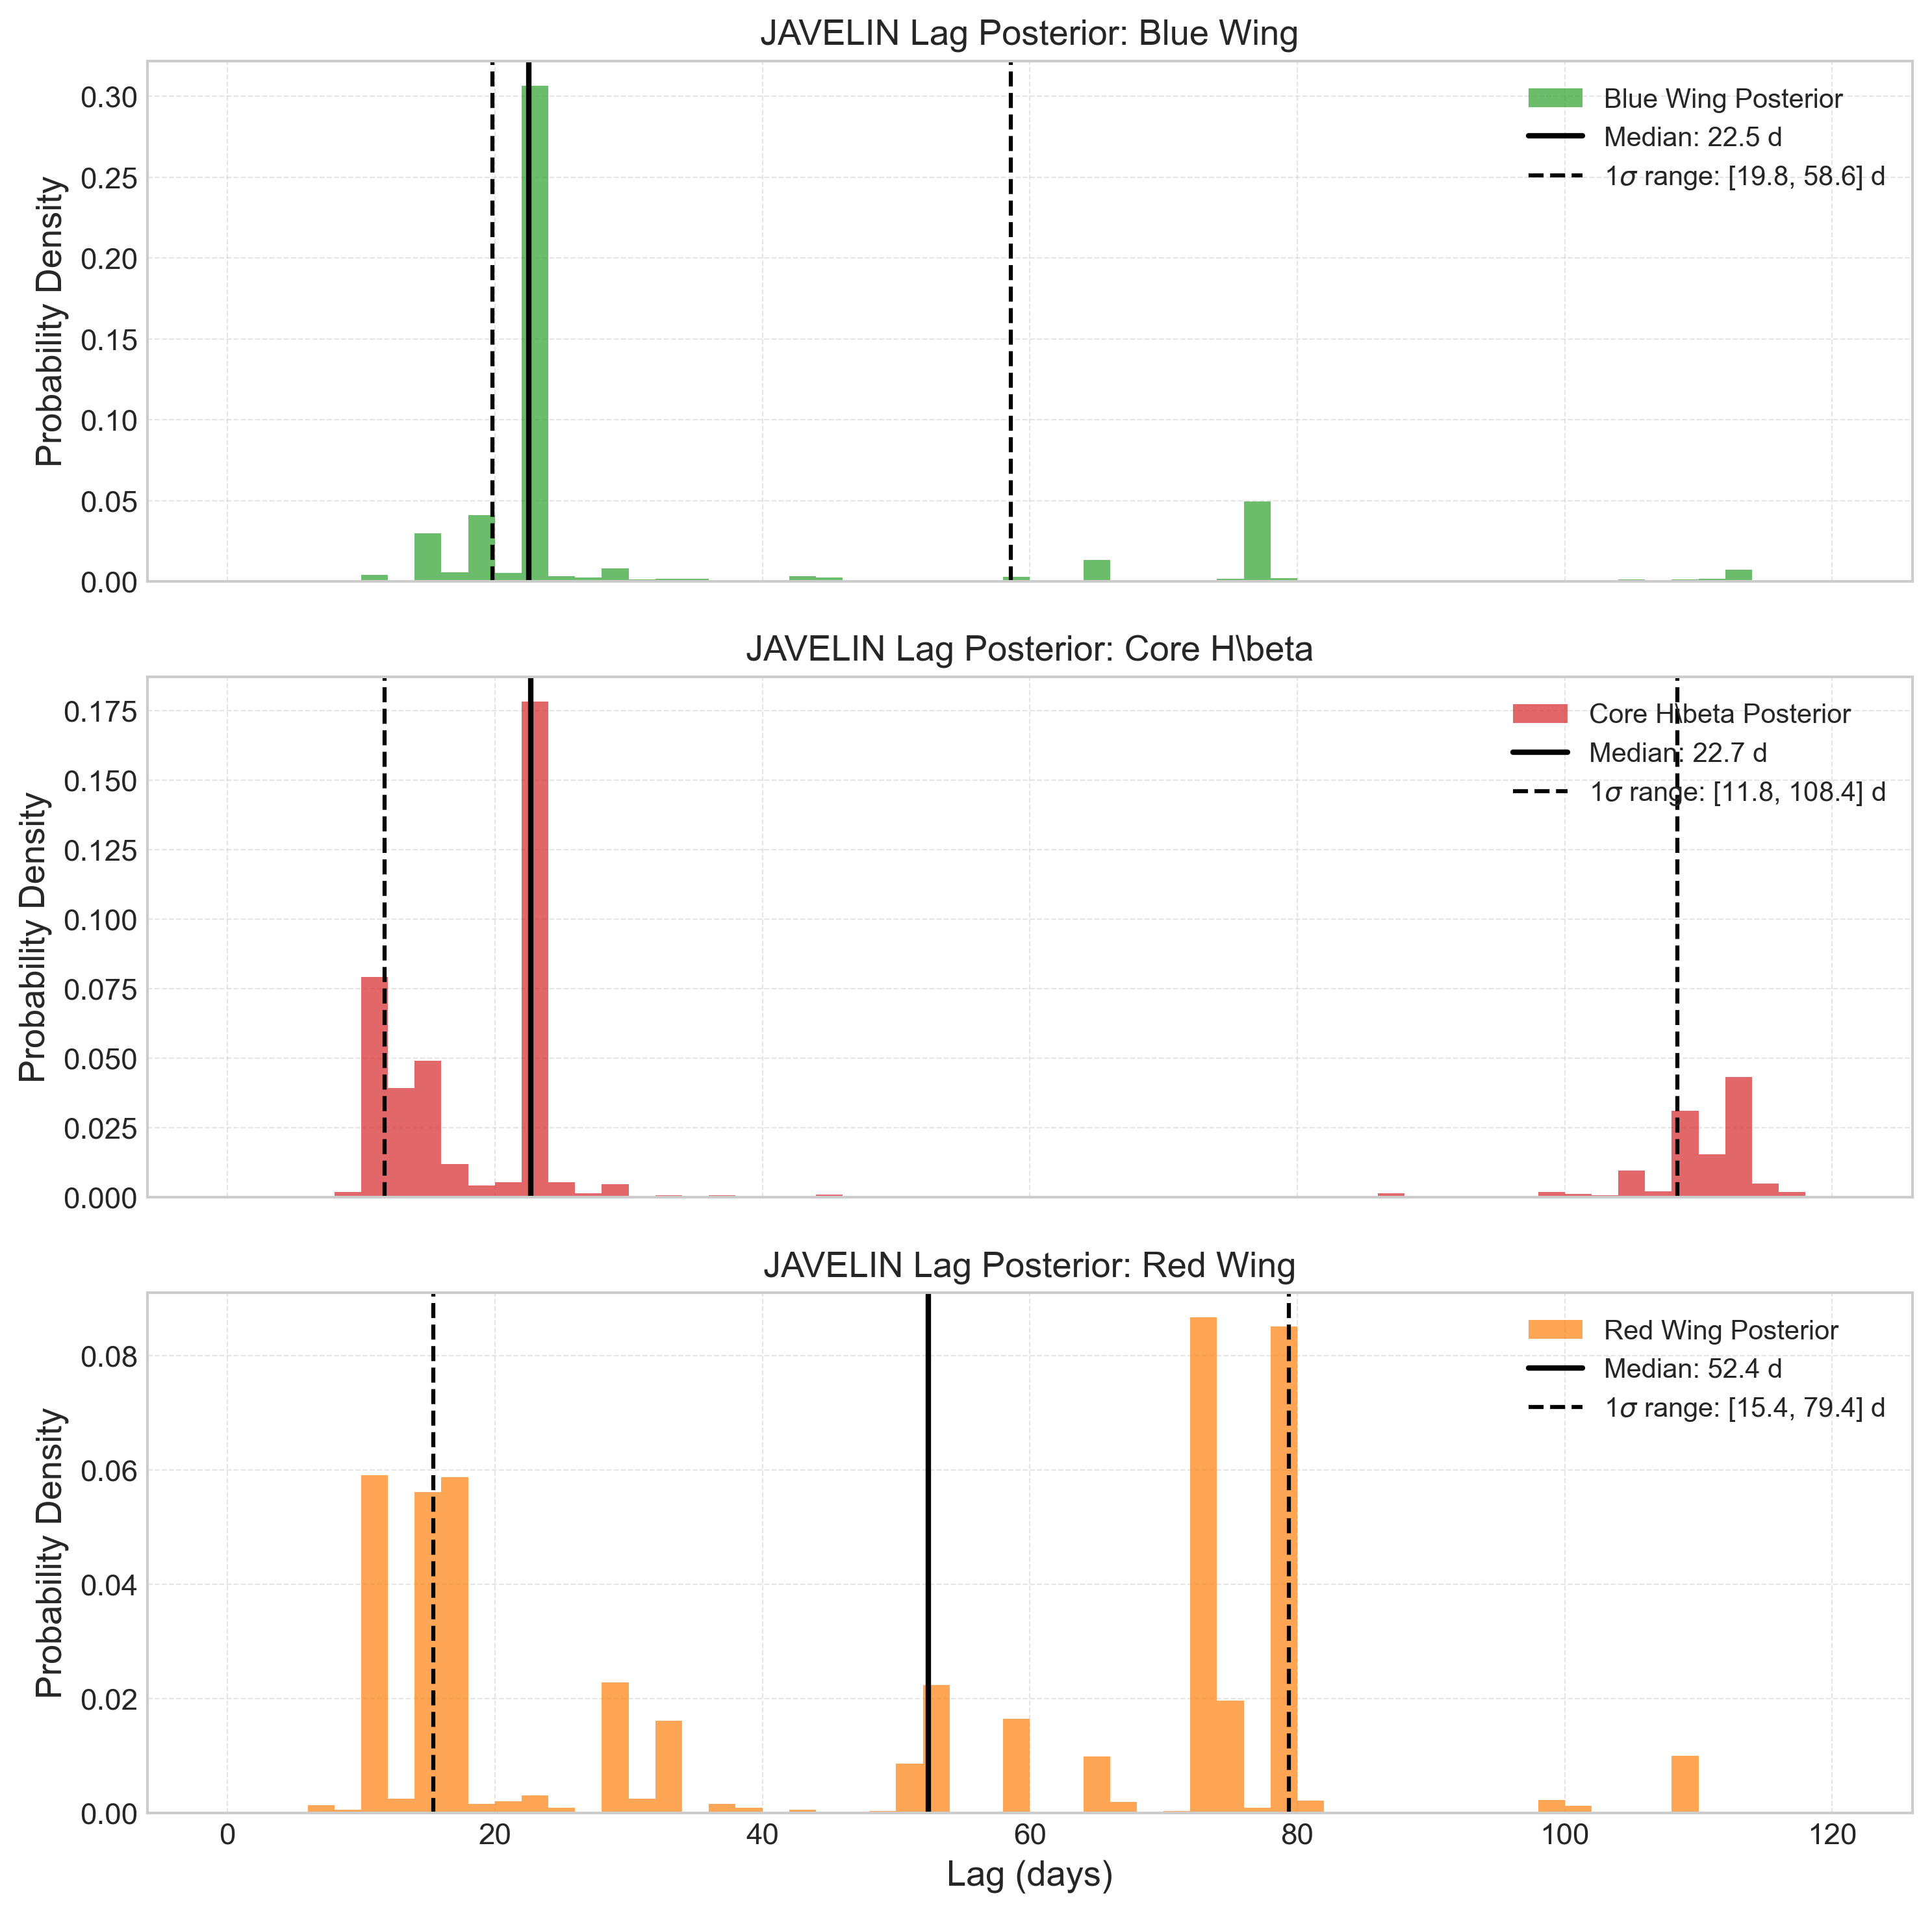
\includegraphics[width=0.8\textwidth]{figure6_javelin_posteriors.png}
\caption{Archived JAVELIN lag-chain histograms. The multimodal chains are shown for transparency only and are not used for inference.}
\label{fig:javelin_appendix}
\end{figure*}

\bibliographystyle{mnras}
\bibliography{refs}

%\bibliographystyle{unsrtnat}
%\bibliography{refs}

\end{document}
